\documentclass[english]{tktltiki}
\usepackage[pdftex]{graphicx}
\usepackage{subfig}
\usepackage{url}

\usepackage{listings}
\usepackage{pifont}
\usepackage{tabularx}
\usepackage{booktabs} %for top, middle and bottomline
\usepackage{multirow}
%\usepackage{array}
%\usepackage{bigstrut}
%\setlength\bigstrutjot{3pt}

\usepackage{amsmath}
\usepackage{algorithm}
\usepackage{algpseudocode}
\usepackage{bbm}

\begin{document}
%\doublespacing
%\singlespacing
\onehalfspacing

\title{An SDN Platform for Traffic Offloading}
\author{Yanhe Liu}
\date{\today}

\maketitle

\numberofpagesinformation{\numberofpages\ pages + \numberofappendixpages\ appendices}
%\classification{\protect{\ \\
%A.1 [Introductory and Survey],\\
%I.7.m [Document and text processing]}}

\keywords{traffic offloading, software-defined networking, WiFi networks, cellular networks}

\begin{abstract}

Cellular networks are facing a data explosion posed by the increasing bandwidth demand of current mobile applications, and cellular operators are trying to leverage auxiliary networks and offload mobile data for relieving this challenge. However, traffic offloading without comprehensive controlling may result poor network utilization and undesirable user experience. In this thesis, we design and implement an integrated architecture for intelligent traffic offloading over collaborative WiFi-cellular networks. Motivated by our measurement, we formulate a mathematical model to estimate and evaluate potential offloading throughput based on various wireless context information, like AP signal strength and bandwidth. To efficiently manage traffic and collect information, we use a centralized SDN architecture in our design. The proposed system enables mobile devices to choose the most beneficial AP for offloading. The experimental evaluation of our prototype implementation demonstrates that this architecture can achieve optimal traffic offloading by considering different real factors instead of making naive decisions. This effort not only explores the feasibility of context-based traffic offloading, but also provides guidelines for designing and implementing a centralized SDN platform for wireless networks.


\end{abstract}

\mytableofcontents


\section{Introduction}

Recently, we are experiencing an explosion of mobile data traffic attributed to a large growing number of mobile-connected devices and data consuming applications. According to Cisco's recent report \cite{cisco14}, global mobile data traffic has reached 1.5 exabytes (1.5 billion gigabytes) every month at the end of 2013, which grew nearly 80 percent during 2013. As an illustration, Cisco predicts that the global mobile data traffic will increase 11 times between 2013 and 2018, and the monthly traffic will surpass 15 exabytes by 2018. The main drive behind this considerable growth is the explosive increase in smart mobile devices and new mobile applications. As reported, there were over 526 million new mobile devices and connections added in 2013, and mobile video traffic has exceeded 50 percent.

To support this increasing traffic in mobile networks is quite challenging. One possible solution is to upgrade current network capacity. Nowadays operators are rolling out their next-generation networks such as LTE (Long Term Evolution) and WiMax to increase average cellular bandwidth. However, this may not promise an economical result both for users and operators. Even in 4G networks, bandwidth is still a limited resource under a flat price structure. When users are paying flat rates for data usage, the operators cannot obtain more from customers for extra data consumption. It is hard to balance end-user requirements and upgrading investments as well as operating costs of cellular networks.

Another feasible solution for this explosive traffic is offloading mobile data to auxiliary networks. For example, offloading traffic from cellular to WiFi can reduce mobile data in cellular networks, and may gain better performance. For operators, it is extremely cheaper to build more WiFi hotspots than cellular network upgrading. In addition, current networks have provided a superb environment for WiFi offloading. For instance, more and more organizations have already deployed a lot of WiFi access points (APs), which means users can easily find an auxiliary WiFi spot to transmit mobile data. As reported by Cisco \cite{cisco14}, 45 percent of mobile data was offloaded to a fixed WiFi or femtocell network in 2013, and they predicts that the percentage will continue to increase. 

Because of the economical benefits and potential, researchers proposed some mobile offloading schemes over WiFi or opportunistic networks. For example, Wiffler \cite{bmv10}, an early attempt on vehicular networks, makes offloading from cellular networks to WiFi networks. MultiNets \cite{nnh+14} is another mobile offloading extension which evaluates WiFi offloading destinations mainly based on their signal strength and connectivity status. In addition, there are some other offloading systems mainly designed based on a DTN (Delay Tolerant Network) approach (e.g. MoSoNets \cite{hhk+12}), which exploit offloading scenarios where applications do not immediately require real-time data transmission. However, those schemes are only designed and operated with limited knowledge of networks, and may result bad transmission performances after offloading. For example, Wiffler and MultiNets only make offloading decisions based on historical bandwidth records and signal strength, but these kinds of information cannot reflect the present traffic load of a certain AP. If mobile users only use those types of data to make offloading decisions, there are high chances that their choices are non-beneficial, or even harmful.

To address this problem, we present a new platform for traffic offloading with a global network view. This platform is based on a software-defined-networking (SDN) approach, where cellular and wireless resources are managed by a centralized controller implemented on Floodlight\footnote{Floodlight. \url{http://www.projectfloodlight.org/floodlight/}}. In SDN, the network control plane is decoupled from the physical devices with well defined programmable interfaces and a centralized global view of networks. This is just what we require in a traffic offloading system: data traffic is controlled and monitored by a central controller, and offloading decisions are made based on the information gained by the controller. Our platform can handle mobile data offloading from cellular to WiFi networks, and also achieve dynamic bandwidth and user allocation among WiFi networks. In addition, this platform takes into account the challenges of wireless mobility and software portability, and implement a general wireless local agent based on Click Modular Router \cite{click}.

The research work is driven by a measurement-based methodology. To design a practical traffic offloading system, we first conduct several different measurement experiments on WiFi and cellular networks. Motivated by those real-world measurement results, we design a context-based offloading decision algorithm in our system, formulate a mathematical model to estimate and evaluate offloading throughput, and implement a prototype platform to verify its feasibility. The evaluation shows that our proposal system may achieve optimal offloading by considering different real factors, and avoid non-beneficial offloading decisions.

The rest of this thesis is organized as follows. Chapter 2 provides an overview of traffic offloading. Chapter 3 describes some fundamental concepts and background knowledge on SDN, and introduces some existing mobile and wireless SDN systems. The design idea of our SDN platform is explained after a measurement study in Chapter 4. Chapter 5 illustrates important implementation details of our platform, and presents testing results obtained from an evaluation of this platform. Finally we conclude this thesis in Chapter 6.

\newpage

\section{Traffic Offloading}

In this chapter, we focus on the problem of traffic offloading, and review its background and some related research work. In addition to cellular data offloading techniques, we extend our topic to re-association based wireless load balancing, and consider it as a subfield of traffic offloading.

\subsection{Background and Motivation}

Current cellular networks are overloaded with explosive traffic generated by increasing mobile devices and various bandwidth-consuming smartphone applications (e.g., video streaming applications, like YouTube, which demand high network throughput). Reported by Cisco \cite{cisco14}, there was 406 million new smartphones added into networks in 2013, and the average amount of traffic used by every smartphone has increased to 529 MB per month. It is forecasted that the number of mobile-connected devices will exceed the number of people on earth by the end of 2014, and the average traffic generated by smartphones will reach to 2.7 GB per month by 2018, which is 5 times more than today's average load (539 MB).

To solve this explosive traffic growth problem, the most straight-forward solution is to scale the network capacity by upgrading cellular systems. As we state in chapter 1, many network operators are promoting their new-generation cellular networks like LTE and WiMax. However, simply increasing network speed may not always be economically effective. Bandwidth resources may still be limited even in 4G networks due to increasing user demanding, let alone large investments and operating costs for upgrading the whole networks.

Instead of simply upgrading network capacity, offloading mobile data to auxiliary networks (e.g. WiFi networks) seems to be a feasible solution which can be quickly implemented at this moment. We have described that mobile offloading via WiFi is a very promising area both in research and industry fields in chapter 1. It is significantly cheaper to deploy new WiFi access points than cellular network upgrading, not to mention that many users have already installed their own WiFi APs at home or office. As illustrated by Lee Kyunghan et al. \cite{lly+10}, we are living in an environment with great WiFi connectivity. In their experiment, users may have available WiFi connections for more than 60\% time of a day, and at any time, nearly 70\% of users stay in a WiFi coverage area, which means users can easily find an auxiliary WiFi spot for data offloading. They also make some trace-driven simulation, and show that WiFi is able to offload about 65\% of the total mobile data with their data, and save 55\% of battery power without delaying transmission.

In addition to mobile data offloading, there is another type of traffic offloading scenario: re-association based WiFi load balancing. In conventional IEEE 802.11 wireless LANs (WLANs), clients select and associate with access points only based on local information like signal strength, which may lead unevenly-distributed traffic loads and poor performance \cite{bc03}. For example, clients in a conference room tend to select the same AP with the best signal level and may suffer traffic congestion, while other adjacent APs may carry very light loads. To address this problems, researchers propose many different schemes to dynamically balance the load across multiple WiFi APs and provide fair services to clients. Since clients may need to re-associate with other APs, it is similar to mobile data offloading where traffic is offloaded from cellular access points to other different access points.

\subsection{Cellular Data Offloading}

As one of the most important parts in traffic offloading, cellular data offloading is always a hot topic both in research and industry fields. Motivated by its economical potential and benefits, many different works are proposed for cellular data offloading.

\subsubsection{Wiffler: Augmenting Mobile 3G by Using WiFi}

Wiffler \cite{bmv10} is a mobile offloading system mainly designed for vehicular networks. As an early attempt, it does not only propose a feasible offloading technique, but also shows some important features which need to be taken into account in offloading design. In general, the simplest policy for mobile offloading via WiFi is to transmit data in WiFi networks when available and switch back to cellular networks when WiFi networks are not available. However, this simple policy may not work well for vehicular networks. As illustrated in their paper, the availability of WiFi is much poorer than that of 3G cellular networks in a moving vehicle. According to their test results, WiFi access is only available 11\% of the time, while 3G access is able to work 87\% of the time. This notably limits the traffic load that can be offloaded to WiFi networks. In addition, they find that the WiFi average throughput for vehicular users is much lower than 3G. If applications simply offload data via WiFi networks irrespective of packet loss rates, they will definitely hurt user experience.

To overcome these availability and performance challenges, Wiffler introduces some key techniques for data offloading: 

\begin{enumerate}
  \item \textbf{Leveraging delay tolerance}. According to their test, the availability of WiFi increase to 30\% with 60-second intervals, which makes offloading from 3G to WiFi more feasible. Also, a user may be willing to tolerate a few seconds delay for sending emails or downloading a file if it can reduce cellular bandwidth usage. Instead of transmitting data immediately, Wiffler introduces delay timeouts, and waits for WiFi to send data before those timeouts.
  \item \textbf{WiFi throughput prediction}. Before transmitting data via WiFi connections, Wiffler uses a simple method to predict future WiFi throughput, and offloads only if WiFi can really save 3G usage within the delay tolerance. It predicts the number of APs one user will meet in the next time interval based on the average number of meeting APs in the past interval, and estimates the average throughput for the future APs based on the historical throughput observed in the past interval. For example, if a user met 4 APs in the last 120 seconds, Wiffler predicts that it will encounter 2 APs in the future 60 seconds. 
  
This simple prediction scheme comes from the observation that APs are always densely located in the same areas. For example, if a mobile user met a lot of APs in the past 5 minutes, he/she is likely to continue to meet new APs in the next 5 minutes (perhaps because it is in a urban area with many APs, e.g. city center).
  
  \item \textbf{Quickly Switching from WiFi to 3G}. Wiffler switches back to cellular networks if WiFi is unavailable within a delay window. The functionality is implemented in a low-level program, which performs very fast.
\end{enumerate}

Though Wiffler proposes a feasible way to offload data in vehicular networks, it may be not suitable for some other scenarios. As illustrated by Lee Kyunghan et al. \cite{lly+10}, the average WiFi temporal coverage is much higher than 11\%. In their experiment, the average temporal coverage of available WiFi spots for all day usage is about 70\% per user. This huge difference may be caused by different measurement scenarios: Wiffler's tests are done mainly by using war-driving, while Lee et al. focus on the natural mobility of users. Typically, a user does stay inside a car or bus for quite long time, but spends a lot of time in office or at home, where the user is likely to have available WiFi access points. 

\subsubsection{MADNet: An Energy-Aware Offloading System}

Different from Wiffler's scheme which is only based on client-side information for offloading , Aaron Yi Ding et al. \cite{dhx+13} propose a collaborative mobile data offloading architecture which is mainly designed for extending mobile battery life. It does not only use a client module on mobile devices, but also introduces two proxies in both WiFi networks and cellular access networks. The three components work collaboratively to decide when and how a client shall offload its cellular data to WiFi networks. Figure \ref{fig:madnet} shows the three major software components of MADNet.

\begin{figure}[htbp]
  \centering
  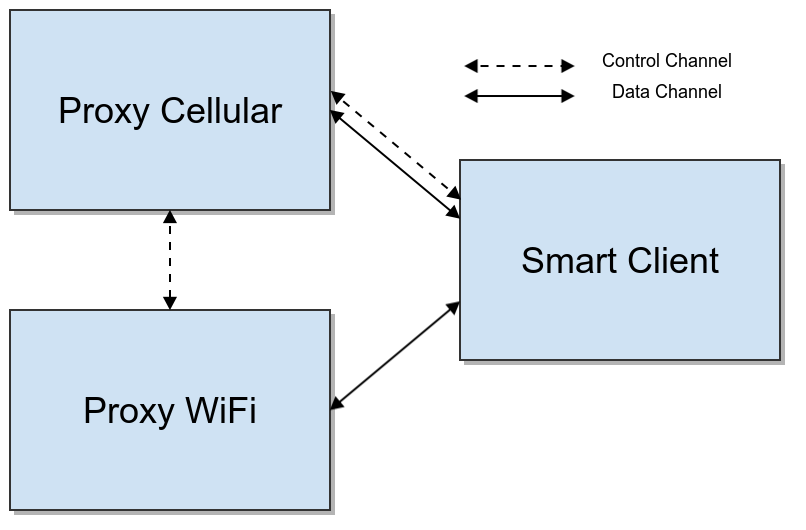
\includegraphics[width=0.6\textwidth]{images/madnet.png}
  \caption{Basic Structure of MADNet \cite{dhx+13}}
  \label{fig:madnet}
\end{figure}

According to the authors' measurements, mobile devices may consume more energy to transfer the same amount of data via a low throughput WiFi connection than that over a high speed 3G access. If applications simply offload as much data as possible via WiFi networks without considering throughput conditions and energy consumption, it may result a shorter battery life for a mobile device. To avoid bad decisions on offloading and selecting WiFi access points, Wiffler uses a simple scheme to predict future WiFi throughput, and if the prediction shows a bad throughput potentially, Wiffler tries to use cellular networks instead. However, it is probably inaccurate since Wiffler only uses historical average throughput to predict future bandwidth for different WiFi access points which may be totally unrelated.

In MADNet, a mobile client first sends its location and mobility information to the corresponding cellular proxy when it wants to fetch contents from the Internet. Then the cellular proxy determines whether the mobile device can potentially save energy by offloading cellular data to a given WiFi AP. If the offloading is determined to perform, the proxy also notifies the candidate WiFi proxy to pre-fetch contents. All the computational tasks on evaluating offloading candidates are moved to the cellular proxy. Since the proxy knows the client's location and neighboring WiFi APs, it may give a better choice on offloading. After receiving the offloading decision and the information about the objective WiFi AP, the mobile client can switch to WiFi networks and continue downloading.

MADNet only performs WiFi data offloading when it predicts that receiving data from WiFi APs saves more energy than transmitting them via cellular networks. It also takes into account the extra energy consumption caused by WiFi offloading and interface switching. For making offloading decisions, MADNet mainly uses the following model to decide whether it is beneficial to offload to a specific WiFi AP:

$$ E_{T} + P_{3G} \cdot C_{W} / B_{3G} - P_{W} \cdot C_{W} / B_{W} > k \cdot E_{oo} $$

and if this inequality holds, it will ask the client to offload to this AP, or otherwise it will continue to check other WiFi APs.

\begin{enumerate}
  \item $ E_T $ is the head and tail energy consumption for mobile devices. Typically, a 3G interface resumes staying at high power after transmitting or receiving a packet, and then drops back to low power only after it has been idle for few seconds. This kind of power consumption caused by state transition is represented as $E_T$ here.  
  \item $ P_{3G} \cdot C_{W} / B_{3G} $ shows the energy consumption if it downloads a file via 3G cellular networks. $P_{3G}$ is the transmitting power of 3G interface, and $C_W$ is the size of the desired file. $B_{3G}$ is a predicted throughput value of 3G networks, which can be estimated from the historical maps between throughput and location.
  \item $ P_{W} \cdot C_{W} / B_{W} $ represents the estimated energy consumption if the download goes through WiFi networks. Similarly to cellular energy consumption, $B_{W}$ is a estimated throughput value of a specific WiFi access point. MADNet can calculate this value from devices' historical mobility and throughput records.
  \item $k \cdot E_{oo}$. $E_{oo}$ is the offloading related overhead, and $k$ is a constant for accommodating measurement errors. Typically, this shows the extra power consumption caused by offloading.
\end{enumerate}

In general, this model compares the power consumption of cellular networks and WiFi networks, and check whether offloading can bring more energy saving when the overhead is also considered. Based on this algorithm, MADNet may avoid to offload mobile data to low-throughput WiFi networks.

\subsubsection{MultiNets: Real-Time Interface Switching}

MultiNets is a seamless offloading system that is mainly designed for real-time network switching \cite{nnh+14}. It focus on seamless interface switching, which is quite different from Wiffler and MADNet that we introduced before. MultiNets enables a mobile device to automatically switch to the most suitable network interface based on user-defined policies (energy saving, data offloading, or performance) without interrupting running applications. Real-time here stands for switching network interfaces in real time without delay. Unlike Wiffler, MultiNets does not introduce delay tolerance for offloading.

Seamless offloading from one wireless interface to another is not as easy as it seems to be. Simply turning off the old interface and turning on a new one may result connection interruption and data loss, which probably hurts user experience when they try to load web pages or play online games. In addition, it may be more challenging to switch connection-oriented data from one interface to another without interruption. For example, an established TCP connection will be closed if the interface being used is turn off, and if we try to use a new interface to resume data transmission, we have to re-initialize new TCP sessions.

To address challenges of seamless offloading, MultiNets proposes a interface switching mechanism mainly for TCP sessions without changing current network protocols. This switching mechanism is designed based on some mobile traffic features concluded from a 3-month-long study, which shows that almost all (99.7\%) mobile traffic is TCP, and the average lifetime of TCP sessions is about 2 seconds, as well as the average concurrency of active sessions is smaller than 2. These features of short lifetime and low concurrency means that we can remain ongoing TCP sessions in the old interface until they finished before finally switching:

\begin{enumerate}
  \item MultiNets counts and records the total number of ongoing TCP connections on the old interface before offloading starts.
  \item If there is any ongoing TCP session, MultiNets first adds new routing table entries for all of them by explicitly specifying to still use the old interface. This makes sure that the ongoing TCP sessions remain working via the old interface.
  \item Then Multinets turns on the new interface, add new routing table entries for it, and replace the default gateway with the new interface. From now on any new connections will be sent via the new interface.
  \item MultiNets waits for a given timeout before tearing down the old interface. It tries to resume these connections without interrupting them during switching. Finally it completely moves on to the new interface.
\end{enumerate}

MultiNets is designed and implemented on the Android platform. It consists of three foundational components: Switching Engine, Monitoring Engine and Selection Policy. The switching engine is the main module which performs the switching between cellular and WiFi. The Monitoring Engine collects all the necessary parameters for switching (e.g. how many TCP sessions are alive on the cellular interface, the amount of data transmitted and received over WiFi and cellular networks, and battery capacity). The Selection Policy defines how switching operates based on bandwidth and power factors. MultiNets provides three different policies right now by considering different scenarios.

\begin{itemize}
  \item Energy-Saving: this policy is designed for minimizing mobile power consumption. Based on the authors' measurements, they propose a heuristic switching algorithm. Mobile devices connect to cellular networks when they are idle, and MultiNets monitors how many bytes sent over cellular interfaces after applications run. The devices will try to switch to WiFi networks as soon as the total amount of data over cellular networks exceeds a specific threshold. When devices are idle in WiFi networks for a certain period, they will switch back to cellular networks.
  \item Offload: this policy tries to offload as more data as possible via WiFi connections. Devices will switch back to cellular networks if WiFi's signal strength is very poor.
  \item Performance: the object of this policy is to provide better throughput over different networks. It compares different interfaces and networks by using estimated bandwidth values derived from corresponding signal strengths, and choose the better one to offload.
\end{itemize}

\begin{figure}[htbp]
  \centering
  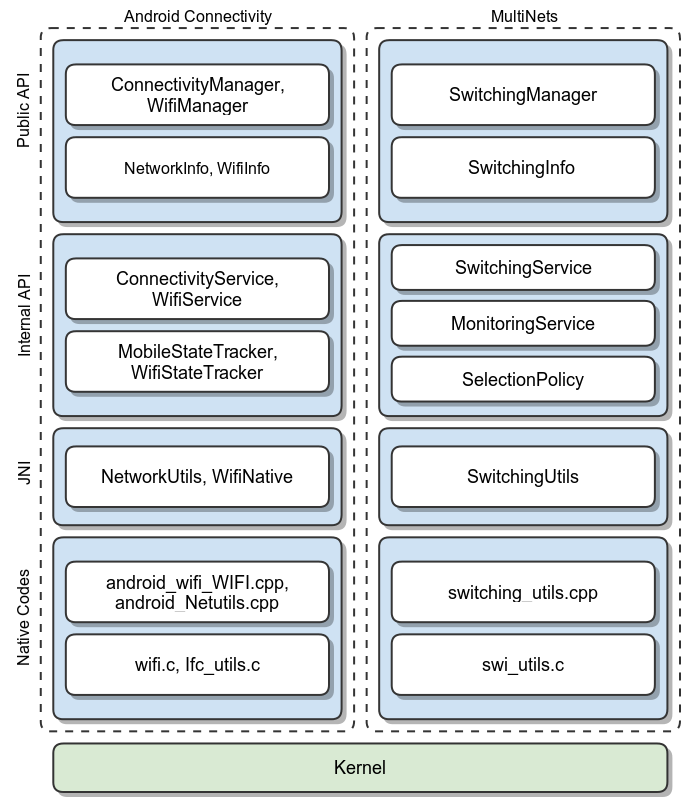
\includegraphics[width=0.8\textwidth]{images/multinets-layer.png}
  \caption{Layered Implementation of MultiNets \cite{nnh+14}}
  \label{fig:multinets}
\end{figure}

Since Android does not support this kind of dynamic network switching, the authors implement MultiNets in a layered style like Android by themselves and hope to provide a general model for various mobile systems. Classes and services of MultiNets are similarly layered as Android's original modules. Figure \ref{fig:multinets} shows the layered implementation of MultiNets. As we can see, some native C/C++ modules that perform lower-level tasks like modifying routing tables are added in Android, and those modules are wrapped into Java API for upper-level applications. As shown in their trace-driven experiments, MultiNets can save up to 33\% energy usage on Android platform in energy-saving mode, or achieving WiFi offloading while reducing TCP interruptions caused by interface switching.

\subsubsection{Other Techniques}

Besides offloading cellular data via WiFi networks, researchers also propose some different techniques based on other complementary networks. Bo Han et al. \cite{hhk+12} design and implement an offloading system based on opportunistic networks. Different from WiFi networks or other networks with fixed infrastructure, there is probably no complete path to forward packets in an opportunistic network. Contents are delivered opportunistically in a store-carry-forward way with the help of human mobility, and device-to-device connections are widely used in opportunistic networks. For example, mobiles can forward data to other devices via bluetooth networks, and reduce mobile data traffic over cellular networks.

In the system proposed by Bo Han et al., mobile users can help to propagate data via opportunistic networks if they meet friends who are also interested in what they have received. Users share data and files within a peer-to-peer transmission range over Bluetooth or WiFi networks. The authors also introduce social participation to their system for enhancing data spreading. Service operators can first choose some active users to receive data through cellular networks, and those active users may have high chances to meet and disseminate data to their friends via opportunistic networks. Experimental results show that their system can reduce the amount of mobile cellular traffic by more than 50 percent with given data traces.

Rather than choosing one interface for global traffic in a mobile device, Brett Higgins et al. \cite{hra+10} propose a different offloading mechanism, which they call it intentional networking. In their scheme, applications provide hints about their traffic semantics by giving some distinguished labels, and the system matches network traffic to the most suitable interfaces based on these labels. For example, game applications may request high bandwidth connections with labels indicating large foreground traffic loads, and the system forward game data via a WiFi interface with better bandwidth. Different from other offloading schemes we explained in the previous sections, intentional networking selects different interfaces and networks for different applications.

To decide which interface is more suitable, they implement a specific process (called as "connection scout") for bandwidth monitoring and evaluation. The connection scout tries to establish network connections periodically over each wireless interface. If a connection is successfully established, it measures the throughput and performance of the corresponding interface. Later, the system chooses interfaces based on latest evaluation results from the connection scout.

\subsection{Load Balancing in Wireless LANs}

Re-association based load balancing, wherein traffic loads across multiple wireless APs can be balanced by dynamically re-assigning clients to different APs, is another kind of traffic offloading applications. There have been some research efforts on this topic. In general, we can group them into two categories: centralized controlling systems and distributed heuristic methods. Nowadays most of the IEEE 802.11 WLAN load balance techniques are using the centralized method in which a central controller makes re-association decisions for clients. The distributed schemes may be more flexible, but always introduce complicated computation tasks on mobile devices. In this section, we mainly focus on the centralized approach, and review some existing research work on it.

\subsubsection{DenseAP: A Centralized Enterprise WiFi Network}

DenseAP, proposed by Rohan Murty et al. \cite{mpc+08} in 2008, is a centralized software architecture for enterprise WLAN deployments. It is designed for current enterprise WLANs where access points are deployed densely (e.g. there may be an AP in every office). To make better association decisions for clients in such an environment with several different available APs in one area, DenseAP system designs a centralized association controlling mechanism. The basic structure of DenseAP is shown in Figure \ref{fig:denseap}. It consists of several programmable  DenseAP nodes (DAPs) which act as WiFi access, and a DenseAP controller (DC) which is the central controller.

\begin{figure}[htbp]
  \centering
  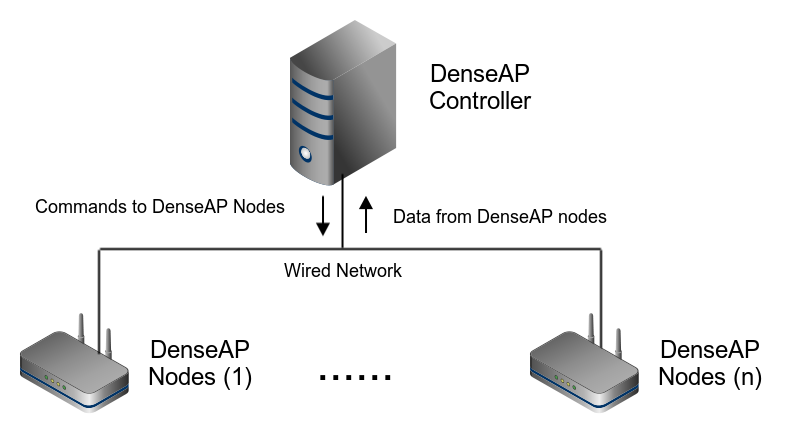
\includegraphics[width=0.8\textwidth]{images/denseap.png}
  \caption{Overall Architecture of the DenseAP System -- several DenseAP nodes are controlled by one DenseAP controller  \cite{mpc+08}.}
  \label{fig:denseap}
\end{figure}

In conventional WLANs, clients make association decisions (select which AP to associate with) only based on local information like signal strength. However, this may result in extremely unfair bandwidth allocation among mobile clients. To improve performance, clients need to connect to different APs even if some APs do not show the best signal strength. In DenseAP, a central controller is used for determining which AP each client shall associate with. As shown in Figure \ref{fig:denseap}, each DenseAP node (DAP) periodically sends summary information about associated clients, current channel conditions and new client requests to the controller. All these periodic summaries sent by DAPs provide the controller with a global view of the whole network. Based on this global view, the controller may choose a suitable access point for each client, allocate channels and perform load balancing.

In current WLANs, clients have to first gather information about available access points before associating, and there are two ways to do that. The first method is called "active scanning", where clients send out Probe Requests on each channel. When APs receive Probe Requests, they will respond with Probe Response messages which include their SSID (Service Set Identification) and BSSID (Basic Service Set Identification). Instead of sending requests actively, clients can just wait for information messages from APs. Typically, APs advertise themselves by broadcasting Beacon frames periodically, and the Beacon frames are similar to the Probe Response frames. Clients just scan all the channels one by one, and listen for incoming Beacons. Once clients obtain necessary information from APs, it decides which AP to associate with mainly based on AP's signal strength. 

For instructing clients to choose suitable access points without any modifications to existing 802.11 protocols, DenseAP uses a "tricky" method to manipulate original WLAN management packets. In DenseAP, the controller performs association control by exposing specific APs to clients selectively. First of all, access points in the DenseAP network do not send out any beacons or only send beacons with a hidden SSID. By doing this, clients have to send probe requests actively before association. Second, each AP in DenseAP maintains a local access control list (ACL) of client MAC addresses. When receiving a Probe request from a client, access points only replies to those whose MAC addresses are listed in the ACL. If an access point receives a request from an unrecorded client, it informs the controller, and the controller determines which access point shall respond to this client. Then, the chosen access point adds the client to its ACL, and sends replies to it. At any given time, one client's MAC address is only recorded in one access point's ACL, which means only one access point is visible to that client.

With this probe response controlling scheme, the association process in DenseAP runs like this: (i) A new client $A$ with MAC address $X$ broadcasts probe requests. (ii) Several different access points receive $A$'s requests, and inform the central controller. (iii) The controller determines which AP the client shall associate with, and notify that AP to add $X$ in its ACL (access control list). (iv) When the client send another probe request again, the chosen AP with $X$ in its ACL responds to the request, and initializes an ordinary association process.

In the association process, the controller is responsible for determining which access point a client shall connect with. To pick the most beneficial access point, the controller in a DenseAP works as follows: first, the controller estimates potential throughput for the client on each different access point. This is a very challenging task since the expected throughput depends on several different factors. Instead of evaluating all these factors, DenseAP mainly focuses on two of the most important ones: \textbf{transmission rate} and \textbf{free air time}, and uses these two metrics to calculate the overall available capacity for access points.

\begin{itemize}
  \item \textbf{transmission rate}: since the transmission rate primarily depends on signal level between clients and access points, DenseAP uses the signal strength (RSSI) of probe requests sent by clients to estimate transmission rates on different access points. When clients attempt to associate, they send out probe requests. Access points report those received requests to the central controller with their RSSI values, and the controller estimates the transmission rate for each access point based on the RSSI value.
  \item \textbf{free air time}: this metric can be used to measure how busy an access point is. The amount of free air time around one access point depends on the traffic generated by this AP. For example, the free air time for one AP may be low when several clients are connecting to it and sending data via it. To calculate the free air time, each AP sends a small broadcast packet periodically at a fixed rate with its highest priority queue (packets in this queue are sent even if there are packets pending in other data queues), and records the delay before the packet is finally sent out from the queue. If the channel is busy, the delay time will be larger than the one caused only by common transmission overhead.
\end{itemize}

Once the controller collects the transmission rate (denoted as $R$) and free air time ($F$) for each access point that receives probe requests, it calculates the available capacity: $Capacity = R * F$, and picks the highest one as the AP for hosting the new client. If available capacities of several DAPs are equal, the controller picks the one that has the fewest clients associated with.

After reviewing how the association works in DenseAP, we can have a glance at how it performs load balancing, which is extended from the basic association process. The controller checks the utilization rate on each access point periodically. It uses the free air time to measure the utilization, and if the free air time of one access point is less than 20\%, it is considered as an overloaded one. When the controller finds overloaded access points, it tries to move some clients on those APs to other idle APs. For example, if an access point $A$ is overloaded, for each client $c \in A$, the controller attempts to find another access point (denoted as $B$) where the expected transmission rate $m$ at $B$ is better (or at least not worse) than that at $A$, and the free air time at $B$ is at least 25\% higher than that at $A$. If such access point is found, $m$ is switched to $B$ following the process described in the association part.


\subsubsection{Dyson: A Client-Cooperated Extension of DenseAP}


\begin{figure}[htbp]
  \centering
  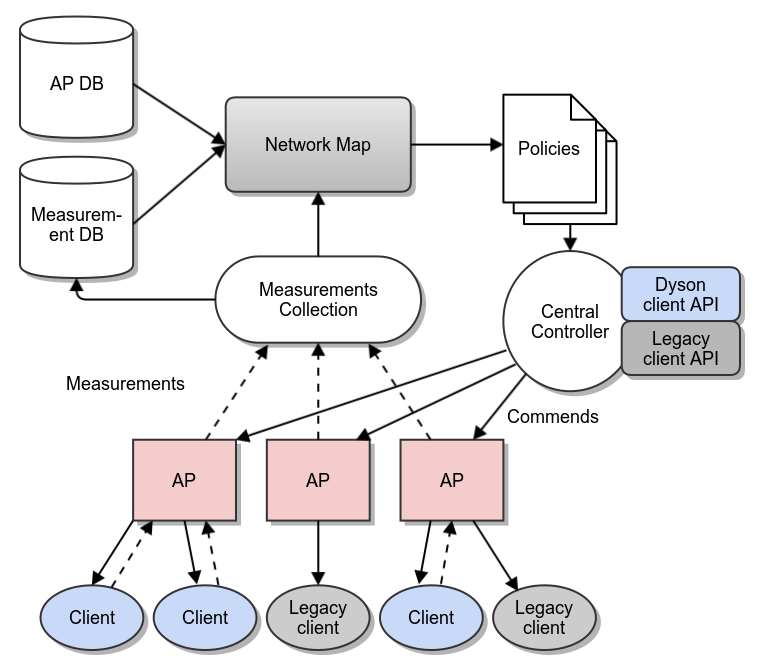
\includegraphics[width=0.65\textwidth]{images/dyson.png}
  \caption{The Dyson Network Architecture -- measurements are collected from underlying devices, and stored in specific databases. The central controller makes management decisions based on those measurement data \cite{mpww10}}
  \label{fig:dyson}
\end{figure}

Dyson is a centralized software architecture for wireless networks \cite{mpww10}. It is extended from DenseAP where no client is involved in the software system. As shown in Figure \ref{fig:dyson}, Dyson consists of a central controller, programmable access points, and two different kinds of clients: Dyson-enabled clients and legacy ones. Both APs and Dyson-enabled clients report measurements to the central controller, and the central controller generates a global view of the whole network based on those measurement data. Like some software-defined networking systems, this global view allows the controller to perform a set of management policies comprehensively. To have better utilization on measurement data, Dyson records them separately in specific databases. 

Though Dyson extends WLANs in a software-defined approach, it still builds upon existing 802.11 standards. One key benefit of Dyson is that it can collect client-based measurements and provide the controller with a better network view. Moreover, legacy clients without the Dyson extension can still be used in Dyson only with reduced functions. Similar to DenseAP, Dyson supports to measure connectivity and channel airtime utilization for each APs. Furthermore, it can also record node locations with the help of Dyson-enabled clients.


\subsection{Research Problems}

After reviewing some existing work on traffic offloading, we realize that almost every method exposes some deficiencies, and suffers from one or more of the following limitations:

\begin{itemize}
  \item \textbf{Inefficient and incomplete offloading decision-making}: as one of the most important part in traffic offloading, decision-making on offloading is studied and explored in every research work we explained in the previous section. Typically an offloading system needs to make two crucial decisions: is it beneficial to offload traffic from one access point to another (or when is it beneficial to do that)? Where shall the traffic be offloaded? 

Although the previous research work provides different decision-making schemes, they may still suffer from non-beneficial offloading decisions. For example, Whiffler determines whether to offload from cellular to WiFi networks only based on historical average throughput of past WiFi access points, which may provide totally unrelated and misleading information for future selection. Some other systems like MultiNets estimates bandwidth for future offloading access points only with their signal strengths. As we discuss before, this may lead very unfair decisions and bad performance. MADNet tries to compare the expected energy consumption in cellular networks and the one in different WiFi networks, but the corresponding bandwidths are still estimated from historical records without considering present traffic loads on each access point. Although DenseAP and Dyson try to measure this kind of real-time traffic loads on APs by introducing free air time, it may take several period to obtain an accurate value, and the suitable offloading time may have been missed.

  \item \textbf{Lack of practicality}: while previous studies have provided many different prototypes for traffic offloading, most of them are mainly designed to solve a part of the problem. Like Whiffler is only implemented for vehicular networks, and MultiNets simply provides algorithms for interface assignment. What we are looking forward to is a practical framework for traffic offloading as an overlay solution over current (or maybe future) cellular and wireless networks.

\end{itemize}

Besides those limitations, some new features may also be required in a new traffic offloading system since seamless offload has been adopted and standardized by Internet Engineering Task Force (IETF) and the Third Generation Partnership Project (3GPP) as a technique in 3G networks.

\begin{itemize}
  \item \textbf{Collaborative management between both cellular and WiFi accesses}: as we mentioned, cellular data offloading and WiFi load balancing show similarities in many aspects (including the decision making, techniques for real-time offloading, etc.), but there are few collaborative controlling systems between cellular and WiFi networks. Most of the work we review in this section are only designed for either cellular offloading or WiFi load balancing.
  \item \textbf{Extensibility}: the system shall be extensible in order to support diverse needs for different networking scenarios. If the system is implemented via a software approach, it shall provide programming abstractions and extensible structures for future development. 
  \item \textbf{Context from users:} mobile users can generate rich contexts with their device sensors, and those contexts may be helpful for traffic management systems. In MADNet and Dyson, users provide some information to the central controller for better offloading decisions, but it seems that we can use more. How can we utilize the rich contexts from mobile users to facilitate the offloading procedure?  
\end{itemize}


\newpage

\section{Software Defined Networking}

In this chapter we give a brief introduction to Software Defined Networking (SDN), which we use as a fundamental concept in our system design. Then we review and discuss some previous research work related to SDN.

\subsection{Background}

Nowadays, computer networks have become exceedingly complex. A large growing number of devices are connected into networks to provide various network services. For common customers, this is definitely good news because they can enjoy rich services, but for network operators and administrators, this is notably challenging. Due to current network architectures, deploying and setting up a large-scale network is anything but not a easy job.

Typically, a networking device (e.g. switch, router, firewall) is architecturally composed of a data plane and a control plane. The control plane decides how and where traffic is delivered by this networking device (which can be considered as the logical "brain" of the device), and the data plane is concerned to forward packets according to the policies defined by the control plane. For example, the policies in a switch's flow table constitute the control plane, and the whole forwarding process can be regarded as the data plane (e.g. looks up destination addresses of incoming packets, determines paths by using the flow table, and delivers packets through the forwarding fabric). As we can see, the control plane and data plane for legacy switches and routers are closely coupled together. 

This integration of control plane and data plane may be beneficial for building a small network with few devices: simple forwarding policies can be easily defined on separated switches and routers, and quickly updated later. However, this may result in big challenges if the network scales to more than hundreds of devices and thousands of hosts. Since the controlling logic is integrated into underlying devices, nearly every device needs to be set up separately. Configuration and management are notably laborious in this scenario, let alone to update the whole network for global changes (e.g. IPv4 migrating to IPv6). The coupling of control logic and data forwarding also hinders innovation of computer networks. To experiment with new ideas and test new protocols in a real large network, researchers have to add complicated configuration carefully to avoid affecting other normal traffic.

In addition, legacy networks are managed through low-level configuration and device-various parameters (e.g. IP addresses and MAC addresses). It is similar to write programs in machine languages in the early days of computers: programmers had to consider everything with very low-level details, which made programs hard to write, port and maintain. Modern operating systems and programming languages have already solved this problems by providing high-level abstractions for low-level resources and information, but legacy networks are still lack common abstractions for underlying resources. Though we use layers to represent the networks, they are not enough for a large-scaled network where configuration and management involve thousands of nodes.

\subsection{OpenFlow: An Enabler of SDN}

In response to the problems we mentioned in traditional computer networks, researchers started to explore new network architectures. OpenFlow, first proposed as a short-term solution for programmable networks \cite{mab+08}, enables to control underlying devices in a software-based approach, and promotes future development on SDN.

OpenFlow defines a standardized way to separate the control and data plane, and provides programmable interfaces for remote management. In traditional networks, forwarding logic is bound to Ethernet devices. In OpenFlow, we can access and manipulate flow tables of Ethernet switches via specialized communication channels from a remote controller. As we can see from Figure \ref{fig:openflow-1}, the logical controller is separated from OpenFlow switch.

\begin{figure}[htbp]
  \centering
  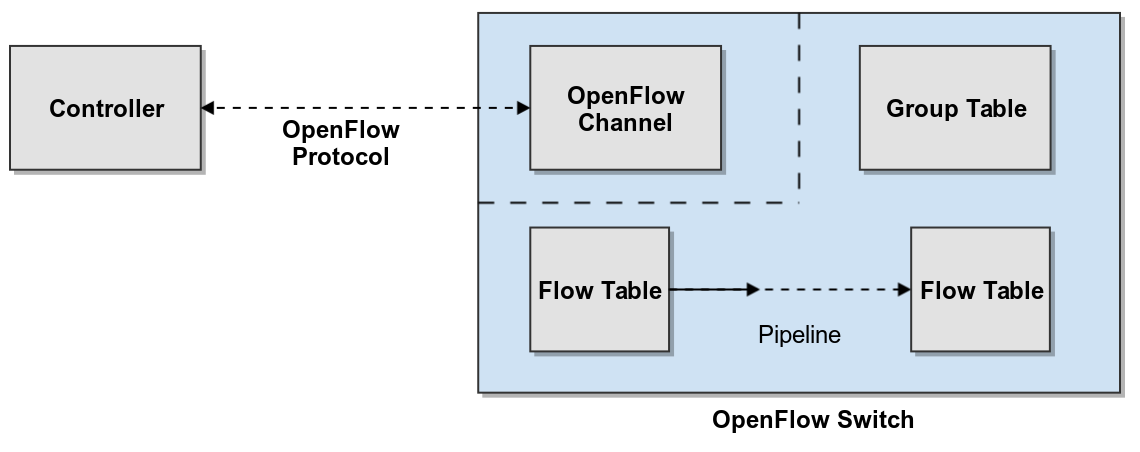
\includegraphics[width=0.9\textwidth]{images/openflow.png}
  \caption{Main Components of an OpenFlow Switch \cite{openflow-1.4.0}}
  \label{fig:openflow-1}
\end{figure}

Figure \ref{fig:openflow-1} also shows two basic components of an OpenFlow switch: one or more flow tables, which perform packet matching and forwarding, and an OpenFlow channel connected to a remote controller. Each flow table contains a set of flow entries with associated match fields, counters and instructions on matched packets. The remote controller can add, edit or delete flow entries in flow tables actively or re-actively (in response to packets and queries) via the standardized OpenFlow protocol.

The basic flow entry for OpenFlow version 1.0.0 \cite{openflow-1.0.0} is shown in Table \ref{tab:openflow-1}. The header fields are used to match incoming packets; the counters record the number of matching packets; actions are the forwarding instructions to apply to matched packets. A flow entry of OpenFlow version 1.4.0 \cite{openflow-1.4.0} includes more specific fields for supporting more detailed information and more complex operations, and it is displayed in Table \ref{tab:openflow-2}.

In general, packets are processed by OpenFlow switches as the following steps:

\begin{enumerate}
  \item Switches perform matching and lookup for every incoming packet according to their flow tables, and if it is matched to one flow entry, the packet will be processed according to the actions defined in that flow entry.
  \item One packet can be matched several times with different flow entries, and actions will be performed sequentially according to the priority of each flow entry.
  \item If no match is found, the switch will perform a default action (e.g. drop the packet, or forward it to a remote controller).
\end{enumerate}


\begin{table}
  \centering
  \begin{tabular}{|l|c|r|}
    \hline
    Header Fields & Counters & Actions \\
    \hline
  \end{tabular}
  \caption{Flow Entry in OpenFlow v1.0.0 \cite{openflow-1.0.0}}  
  \label{tab:openflow-1}
\end{table}

\begin{table}
  \centering
  \begin{tabular}{|c|c|c|c|c|c|}
    \hline
    Match Fields & Priority & Counters & Instructions & Timeouts & Cookie \\
    \hline
  \end{tabular}
  \caption{Flow Entry in OpenFlow v1.4.0 \cite{openflow-1.4.0}}  
  \label{tab:openflow-2}
\end{table}

By introducing programmable flow tables and a standard controlling protocol, OpenFlow switches provide great flexibility to network management and configuration. The control logic and forwarding plane can be separated now with OpenFlow-enabled devices, and we can dynamically set up forwarding policies remotely and programmingly by using OpenFlow, which notably promotes future development of SDN.

\subsection{SDN: Concepts and Structures}

Before OpenFlow was released, researchers had proposed some different control mechanisms aiming to give a global abstract view of networks. For example, 4D \cite{ghm+05} and SANE \cite{cfp+07} are both early attempts for this kind of network abstraction. However, most of them lack general programmatic control of underlying networks. Thanks to OpenFlow, standardized network controllers and network operating systems with general programming interfaces are emerging, and the general concept of SDN becomes more clear.

SDN (Software Defined Networking) provides a revolutionizing networking architecture which moves control logic from underlying devices to centralized controllers. It suggests to build a network in a centralized approach instead of completely distributed ones. In SDN, packet forwarding is controlled by a global controller via programmable interfaces. This is quite different from legacy networks where forwarding policies are bound into underlying devices. A typical SDN architecture is shown in Figure \ref{fig:sdn}. Programmable forwarding devices (like OpenFlow switches) are in underlying networks. The upper network operating system provides an global and centralized view of resources in networks. A network virtualization layer may abstract the global view to higher level ones (e.g. represent network devices by using human readable words instead of IP addresses and MAC addresses), and we can easily develop and maintain control programs based on those abstract views.

\begin{figure}[htbp]
  \centering
  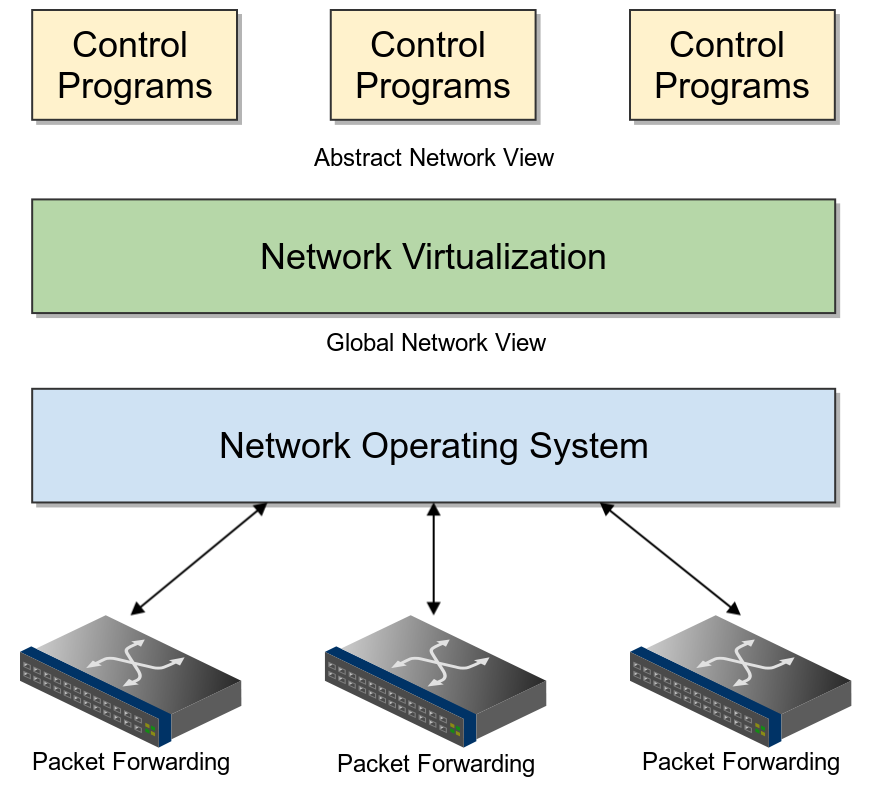
\includegraphics[width=0.7\textwidth]{images/sdn.png}
  \caption{Architecture of an SDN platform}
  \label{fig:sdn}
\end{figure}

Typically, SDN is designed with three most characterizing properties:

\begin{itemize}
  \item Separating the control plane from the data plane: this logic decoupling may simplify network management and provide opportunities for future extension.
  \item Providing applications with a global view of the network and a higher level of abstraction: compared with making decision distributedly, a global view helps controllers to make better choices. Also, it is easier to write management programs with a higher level of abstraction. Image how difficult it will be if you have to write your controlling programs with fixed IP addresses and MAC addresses, not to mention upgrade your programs when those physical addresses changed.
  \item Programmability: the control logic can be defined with software programs. This is one of the most important features in SDN. The first two properties (logic decoupling and abstraction view) also promote a better programming style in SDN. Developers can write more dynamic and flexible controlling programs based on an abstract view of the network, which is much easier to maintain and upgrade in the future.
\end{itemize}

In general, SDN provides great opportunities to solve problems in current networks. It proposes a powerful way to set up network policies by using centralized controllers via programming interfaces, which may free network administrators from boring manual configuration with low-level device-based commands. In addition, it is more easier to introduce new ideas and run experiments in an existing network in a software-based approach.

\subsection{SDN Controllers}

As one of the most important parts in SDN, controllers (or sometimes regarded as network operating systems) are always the hottest topic in both research and industry fields. NOX, the first OpenFlow controller released in 2008 \cite{gkp+08}, is one milestone attempt of SDN controllers. After NOX, many other OpenFlow controllers have been released, like POX\footnote{Pox. \url{http://www.noxrepo.org/pox/about-pox/}}, Floodlight, and Ryu\footnote{Ryu. \url{http://osrg.github.io/ryu/}}. Figure \ref{fig:nox} shows the basic structure of a NOX-controlled network, and most SDN systems follow a similar network architecture: a set of OpenFlow switches are connected to a centralized controller, where management applications run with a global view of the network. The network view is collected and updated by the centralized controller with OpenFlow switches, kept in a database, and used by different applications as their program inputs.


\begin{figure}[htbp]
  \centering
  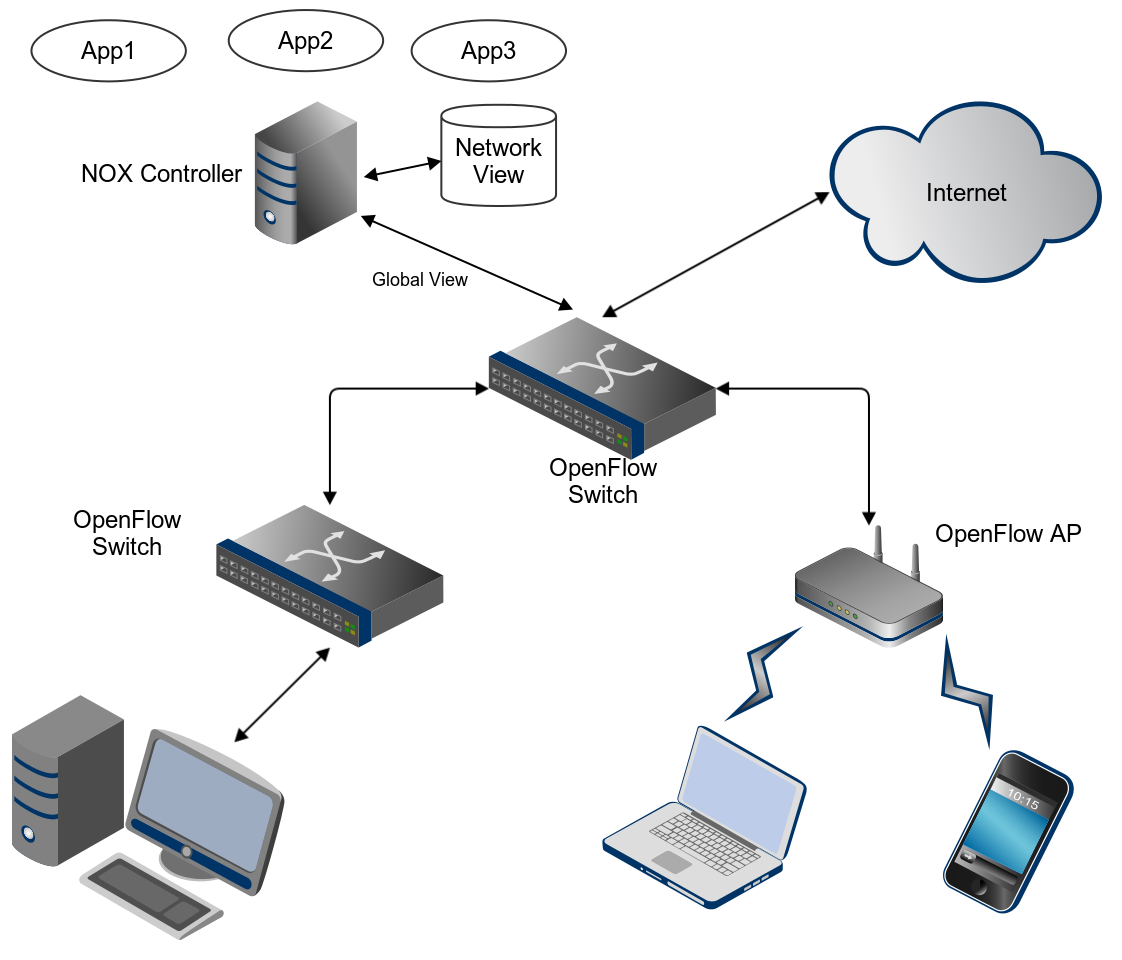
\includegraphics[width=0.7\textwidth]{images/nox.png}
  \caption{Architecture of a NOX-based Network -- OpenFlow switches, a server running NOX and management applications \cite{gkp+08}.}
  \label{fig:nox}
\end{figure}

NOX and many other controllers use standardized events to represent incoming changes happened in underlying networks (e.g. links go up and down, flows arrive and leave). Applications can register specific event handlers to cope with particular changes. When those events happens, logic in corresponding event handlers will be triggered. We show this basic handling process in Figure \ref{fig:beacon} with Beacon \cite{eri13}, a Java-based SDN controller. The controller collects OpenFlow protocol messages, and sends those information to applications registered with a specific OpenFlow monitor service. Then those registered application listeners receive updated messages in a serial pipeline. For example, in Figure \ref{fig:beacon}, the application "Device Manager" first obtains OpenFlow messages, then it can propagate those messages to the "Topology" application. In this way, underlying events can be easily propagated to different applications.

\begin{figure}[htbp]
  \centering
  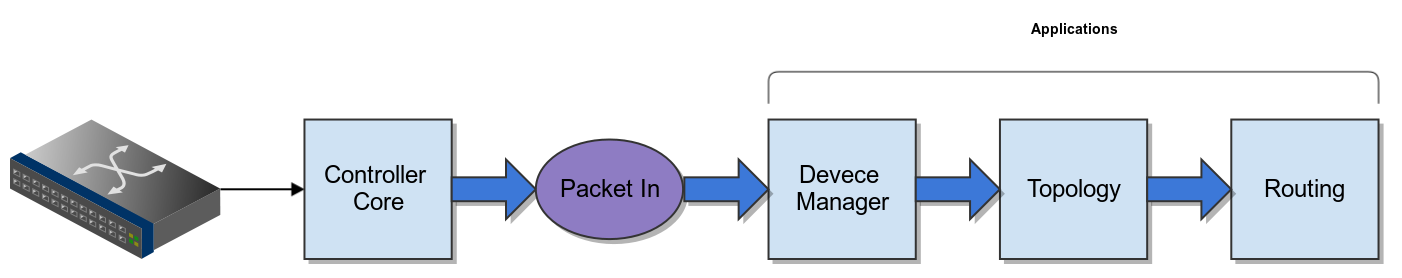
\includegraphics[width=0.8\textwidth]{images/beacon.png}
  \caption{Beacon OpenFlow Signal Handling Pipeline \cite{eri13}}
  \label{fig:beacon}
\end{figure}

In general, the central controller is responsible to collect information from underlying devices, and generate a global view of the network. Extended applications running on the top of the controller use the global view (or a part of the view) to make management decisions, and perform various networking policies. 

\subsection{Towards Better Scalability}

With the development of SDN techniques, researchers start to focus on network scaling. The main initial purpose of a SDN controller is to offer a centralized and abstract view of underlying networks, and increase the productivity for network management and configuration via a software-based approach. However, achieving this transformation from a completely distributed system to a centralized architecture brings considerable challenges of scalability. It is difficult to manage lots of resources only in a centralized way when the size of a network grows. Also, performance can be a bottleneck for a centralized system. For example, if all the underlying switches need to communicate with one central controller, some of them may suffer long latencies if they are far away from the controller in a very large network. For scaling existing SDN systems, researchers have proposed some new structures and techniques for SDN controllers.

\vspace{1mm}

\textbf{Kandoo: A Hierarchical Control Platform}

\vspace{1mm}

\begin{figure}[htbp]
  \centering
  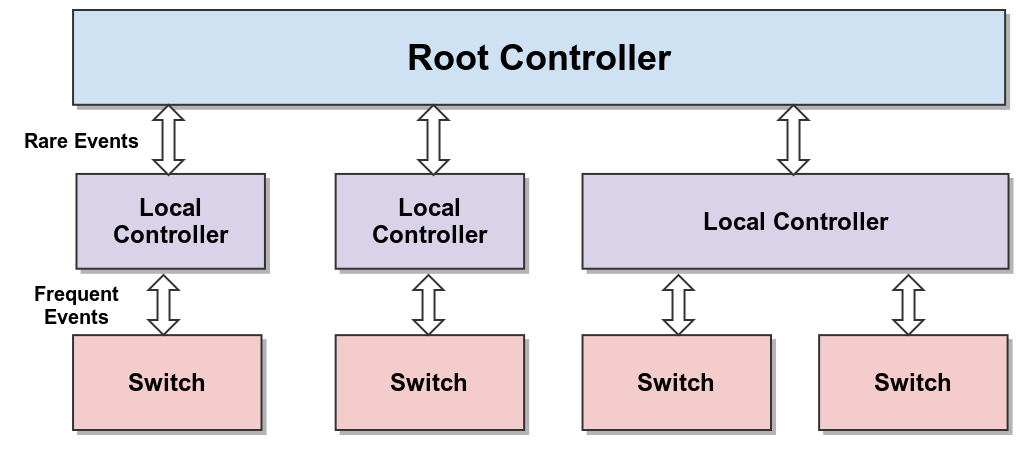
\includegraphics[width=0.7\textwidth]{images/kandoo.png}
  \caption{Kandoo's Two-Level Framework -- local controllers process frequent and local events, whereas a root controller handles other global events \cite{hyg12}.}
  \label{fig:kandoo}
\end{figure}

Kandoo is a hierarchical SDN framework designed for the OpenFlow protocol \cite{hyg12}. It introduces a two-level hierarchical SDN controlling architecture, and separates local configuration and management from global policies. It creates a simple extension for scaling SDN systems: local controllers directly manage OpenFlow switches and execute applications which do not require network-wide views, while a root controller with the global view is responsible for all the underlying local controllers. Figure \ref{fig:kandoo} illustrates this hierarchical framework. For event handling, Kandoo follows the similar idea used in NOX and beacon, and extends it in a two-level hierarchical system. The root controller can subscribe a set of specific events in local controllers, and the local controllers will propagate those events to the root controller when they happen.

\vspace{1mm}

\textbf{HyperFlow: Extending NOX to Distributed Controllers}

\vspace{1mm}

Different from Kandoo's hierarchical centralized framework, HyperFlow proposes a logically centralized but physically distributed SDN controlling system \cite{tg10}. It allows more than one controllers to be deployed in a network, and every controller shares a consistent network-wide view. This structure provides both scalability and control centralization for a SDN system.

\begin{figure}[htbp]
  \centering
  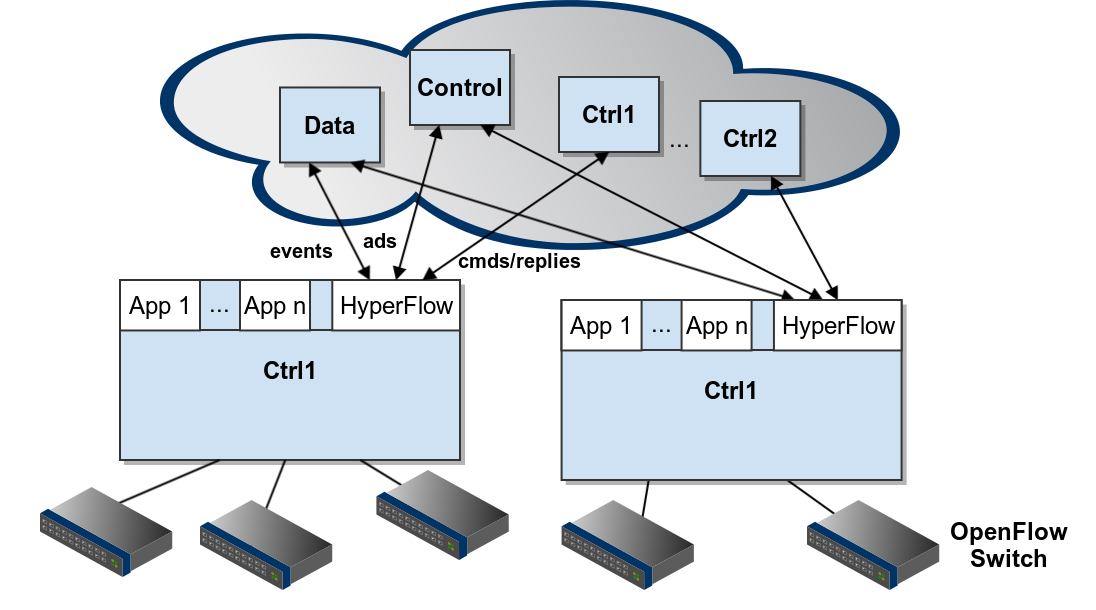
\includegraphics[width=0.8\textwidth]{images/hyperflow.png}
  \caption{Overview of HyperFlow -- the HyperFlow application runs on each NOX controller, and each controller synchronizes events and controlling logic with other controllers via specific channels \cite{tg10}.}
  \label{fig:hyperflow}
\end{figure}

HyperFlow network consists of a set of OpenFlow switches as forwarding plane, several NOX servers running the HyperFlow controlling application as distributed controllers, and an event spreading system for controller communication and synchronization. All the controllers run the same software and have a consistent network-wide view. OpenFlow switches are connected to the best (nearest) controller with shorter response time. If one controller crashes, switches can be logically moved to another controller nearby. Figure \ref{fig:hyperflow} shows the basic structure of a HyperFlow network.

Synchronizing network views is the most distinguishing feature of HyperFlow. It provides a consistent network view by using a event publish/subscribe component. Each controller running HyperFlow publishes traffic/controlling events which are generated locally but affect the global network view to other controllers. In the mean time, other controllers can subscribe those messages from specific communication channels, and replay them for generating a consistent network view. In addition, HyperFlow introduces health checking to SDN controllers for better reliability. Each HyperFlow controller sends advertisements periodically to indicate its state and health. If one controller does not publish those advertisements for several successive intervals, it will be considered as crashed, and the switches which were managed by it will be logically redirected to other neighboring healthy controllers.

\vspace{1mm}

\textbf{Onix: A More Flexible Distributed Controlling Platform}

\vspace{1mm}

Onix is another distributed SDN controlling framework. It creates a distributed data structure called NIB (Network Information Base) to represent network resources. In NIB, each network element is recorded as a set of key-value pairs with a globally unique identifier. For example, a NIB data entry can include a network node with its attributes like link-speed and capacity, and a distinguished id. Onix maintains a consistent NIB for the whole network, and upper-level applications make decisions based on the NIB. This is somewhat alike HyperFlow's shared view of network, but it is more flexible and supports hierarchical topologies. For better scalability and performance, Onix introduces two mechanisms to compact the size of NIB: 

\begin{itemize}
  \item Partitioning: an Onix controller can only keep a part of NIB data in its memory. Since controllers may be only responsible for some devices in a network, they can choose to partition the global network view into small pieces for simplifying control logic and reducing data storage.
  \item Aggregation: Onix supports to represent a set of network devices as one aggregated entry in NIB. This is useful to reduce NIB size for upper-tier controllers in a hierarchy system.
\end{itemize}

To maintain a consistent NIB for the whole network, Onix uses two kinds of mechanisms. For persistent but less dynamic data, it choose a transactional SQL-like database. For networks with high update rates, Onix provides an eventually-consistent memory-only DHT system for the NIB. In Onix, all the controllers share consistent information from the NIB database, and manage a set of underlying devices with various policies.

\vspace{1mm}

\textbf{ElastiCon: An Elastic Distributed Controller Architecture}

\vspace{1mm}

Different from HyperFlow and Onix, Advait Dixit et al. \cite{dhm+13} propose a dynamic pool of SDN controllers to replace static mappings between switches and controllers. They suggest an elastic distributed SDN control platform called ElastiCon where switches can be dynamically allocated to different controllers according to traffic conditions. In ElastiCon, controller nodes are organized into a centralized cluster, and each node is connected to several different switches. A traffic load monitoring application runs on the control cluster, and reports underlying load statistics. When some controllers' loads are beyond their thresholds, ElastiCon will dynamically migrate corresponding switches to idle controller nodes. Based on this dynamic controller allocation mechanism, ElastiCon balances management traffic and provides better scalability.


\subsection{SDN and Wireless}

Compared to Ethernet-switch networks, wireless and cellular networks suffer from more complex control-plane design and configuration. Unlike traditional IP networks, providers in cellular networks have to set up highly customized policies based on various subscriber requirements and user mobility, which exposes big challenges of complexity. With the emergence and evolution of SDN, some researchers try to fix this kind of problems in an SDN approach. 

\vspace{1mm}

\textbf{OpenRoads: An Early SDN Attempt in Wireless Networks}

\vspace{1mm}

OpenRoads \cite{ysk+10} is an early attempt to develop an open and software-controlled wireless platform with OpenFlow and NOX. Similar to existing SDN systems, it separates the control plane and data plane, and moves all the control logic to a centralized NOX controller. For satisfying different user requirements and increasing wireless network flexibility, OpenRoads introduces FlowVisor to slice network virtually. It can be considered as a transparent layer for OpenFlow, which slices networks by selectively rewriting OpenFlow messages for different users and controlling purposes. OpenRoads also provides a SNMP module for quickly configuring underlying nodes via the standard SNMP protocol. Because current OpenFlow protocol is not designed for managing wireless resources, this SNMP module is very necessary and important to control wireless devices.

As shown in Figure \ref{fig:openroads}, different users' traffic loads are separated with different forwarding controlling policies in OpenRoads. In general, OpenRoads provides a complete network framework which can be virtualized to create isolated slices for new experiments or new forwarding policies in a wireless environment.

\begin{figure}[htbp]
  \centering
  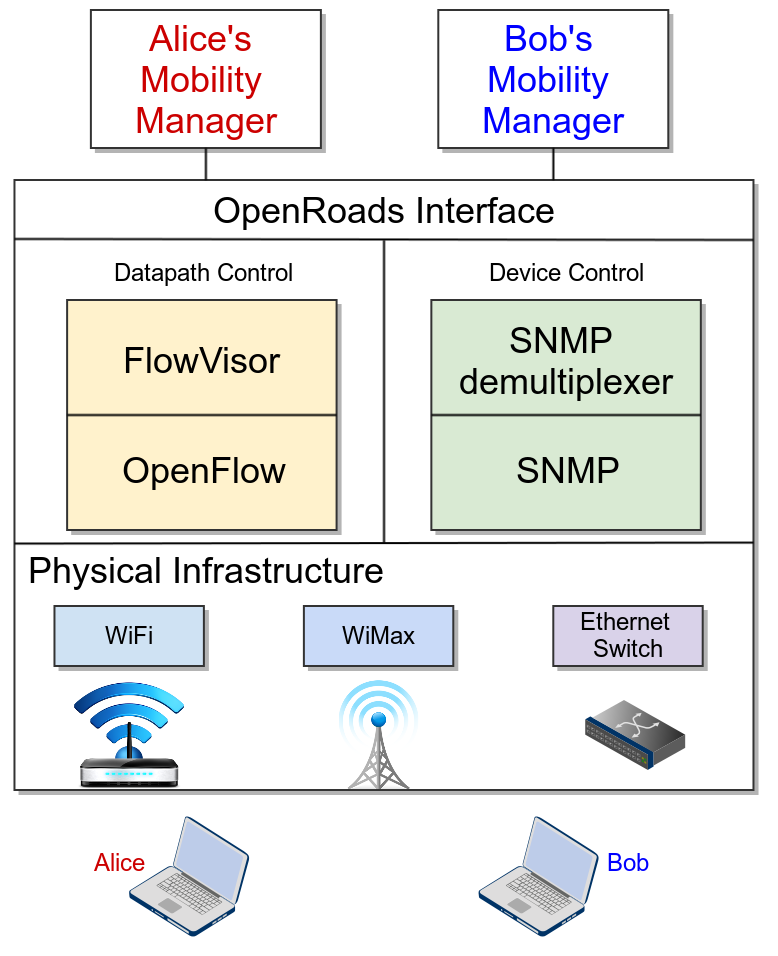
\includegraphics[width=0.5\textwidth]{images/openroads.png}
  \caption{Basic Structure of OpenRoads -- Alice and Bob's traffic loads can be easily separated with the OpenRoads platform \cite{ysk+10}.}
  \label{fig:openroads}
\end{figure}

\vspace{1mm}

\textbf{Odin: Programming Enterprise WLANs}

\vspace{1mm}

Odin is an SDN framework designed for enterprise WLANs (wireless local area networks) \cite{sszm+12}. It is inspired by some projects based on OpenFlow, and goes further in the wireless direction by taking into account peculiarities of 802.11 environments. In a typical enterprise WLAN system, a wide range of services are provided (e.g. authentication, load balance, and mobility management). With Odin, those services can be implemented as programmable applications running on an SDN central controller, and easily updated or modified in the future. 

\begin{figure}[htbp]
  \centering
  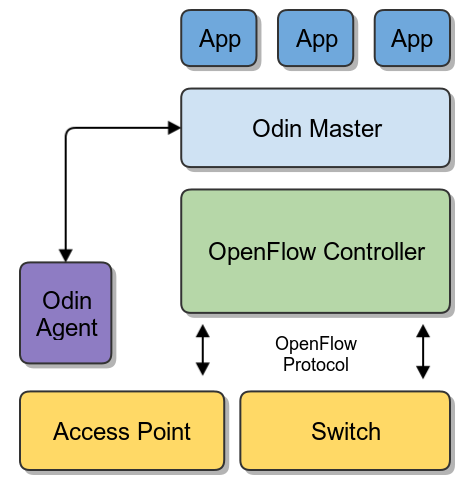
\includegraphics[width=0.5\textwidth]{images/odin.png}
  \caption{Architecture of Odin -- the Odin master runs on an OpenFlow Controller, and communicate with Odin agent with a custom protocol \cite{sszm+12}.}
  \label{fig:odin}
\end{figure}

Figure \ref{fig:odin} shows the basic structure of Odin, which consists of a master component, multiple programmable agents and a set of applications. The Odin master is an application running on the top of an OpenFlow controller, and uses the global view provided by the OpenFlow controller (In Odin's current implementation, Floodlight is chosen as the OpenFlow controller). All the access points and switches are connected to the OpenFlow controller and managed based on the logic of Odin Master. Extended applications can run on the top of the Odin master to use software interfaces exposed by the master. 

Odin also designs and implements software agents on access points, which provides programmability to the association process in 802.11 networks. Like DenseAP \cite{mpc+08}, the Odin master uses agents to perform AP association and manage client allocation. The authors design their own controlling protocol between the master and agents, and use a TCP connection for communication. In their framework, each client is only assigned to one access point by the Odin master, and the master uses a specific data structure (called as LVAP) to record allocation and traffic information for clients.


\vspace{1mm}

\textbf{SoftRAN: An SDN Structure for Radio Access Networks}

\vspace{1mm}

Different from OpenRoads and Odin, Aditya Gudipati et al. \cite{gplk13} mainly focus on the radio access network (RAN) and propose a centralized software-defined radio access network structure named SoftRAN. As an important part of the cellular network infrastructure, RAN is responsible for providing wireless connectivity to mobile devices. Currently the traditional radio access networks use distributed algorithms to figure out how to allocate limited wireless spectrum and avoid interference, which  is a difficult task in a dense-deployed wireless network. 

SoftRAN applies SDN principles to redesign the radio access network: base stations in one geographical area are abstracted as one big virtual base station made up of radio resources, and radio resources are conceptually thought of as elements in a three dimensional grid of index, time and frequency slots. SoftRAN then uses a logically centralized controller to manage all the radio elements on the 3D grid. The controller collects periodic updates from radio elements and maintains a global network view to make control decisions (e.g. assign transmit power).

For improving performance and handling the inherent delay between the centralized controller and different base stations, SoftRAN proposes to move some controlling tasks which are only based on local network views to individual radio elements. In general, it follows two main principles: first, the control decisions affected by other radio elements shall be made by the centralized controller, e.g. handovers, power setting. Second, base stations shall preferably handle those requests which are based on rapidly-changing parameters.

\vspace{1mm}

\textbf{SoftCell: Redesigning Cellular Core Network}

\vspace{1mm}

\begin{figure}[htbp]
  \centering
  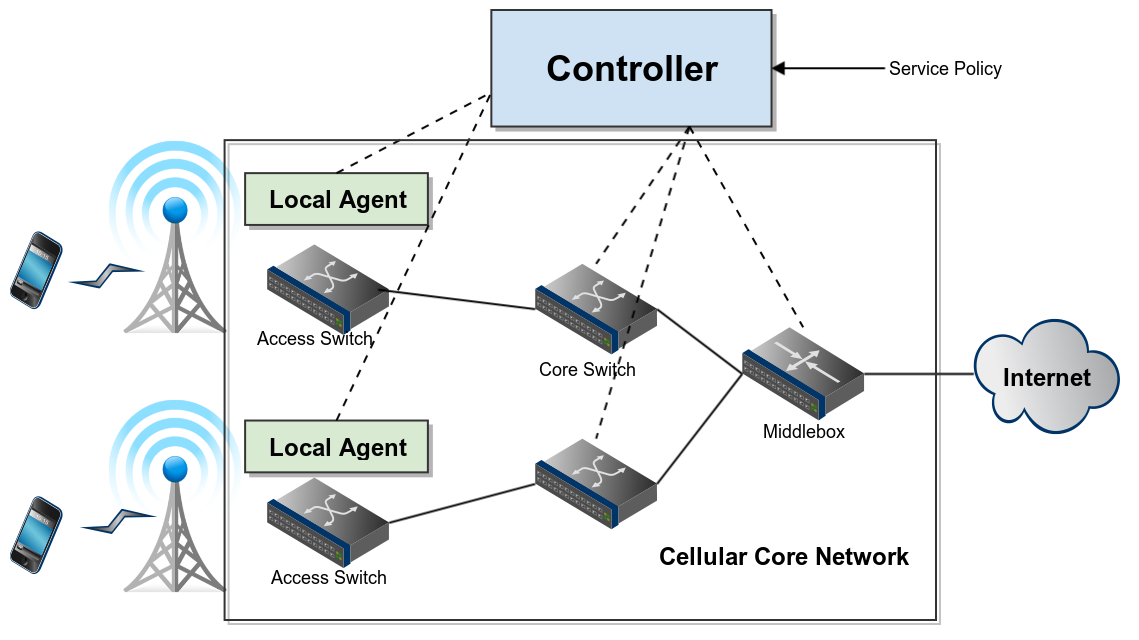
\includegraphics[width=0.9\textwidth]{images/softcell.png}
  \caption{SoftCell Structure -- network devices are divided into three different categories: access switches, core switches, and middleboxes. Each base station is connected to an access switch with a location agent, and the core forwarding logic is implemented by core switches and middlebox. The central controller manages all the underlying devices in a high level \cite{jlvr13}.}
  \label{fig:softcell}
\end{figure}

The SoftCell project \cite{jlvr13} also explores how to use an SDN-based architecture in cellular networks. It tries to redesign a scalable and flexible cellular core network in an SDN approach, which is therefore complementary to SoftRAN that mainly focuses on radio access networks. 

The SoftCell architecture is shown in Figure \ref{fig:softcell}: controlling logic is decoupled from devices to a centralized controller, where various services for subscribers are described in high-level policies, and can be translated to switch-level rules on switches and middleboxes later. Each base station is connecting to an access switch for client packet classification. To reduce interaction latency between access switches and the centralized controller, there will be a local agent near each access switch. It caches packet classifiers and corresponding policies, which can be directly used for forwarding user data. The rest of the network consists of core switches and middleboxes. The core switches are just responsible for packet forwarding based on the policies defined in the centralized controller, and sophisticated packet processing will be done in middleboxes.

In SoftCell, service policies are defined with high-level abstraction, and the controller handles all the low-level details, and converts the high-level languages to underlying rules. Table \ref{tab:softcell} gives an example of high-level policies used in SoftCell.

\begin{table}
  \centering
  \begin{tabular}{|c|l|l|}
    \hline
    Priority & Predicated & Service Actions \\
    \hline
    1 & provider == B & Firewall \\
    \hline
    2 & provider != ! & Drop \\
    \hline
  \end{tabular}
  \caption{Example of Service Policies in SoftCell}  
  \label{tab:softcell}
\end{table}

For better scalability, SoftCell tries to minimize the size of forwarding tables in different switches by aggregating table entries along multiple dimensions: First of all, it can merge entries by underlying location addresses (e.g IP address 192.168.0.1 and 192.168.0.2 can be merged as 192.168.0.0/24). Typically this technique is widely used in OpenFlow switches as wildcard matching. Second, it also designs a way to aggregate rules with high-level tags. For example, "provider == B" in Table \ref{tab:softcell} can be used as a tag to merge entries. In addition, SoftCell supports aggregating table entries by mobile-device ID. 

In one word, SoftCell shows the possibility to redesign and simplify current cellular networks based on an SDN approach, and provides some feasible and cheap techniques for improving the scalability and flexibility of cellular core networks.


\subsection{Summary}

In this chapter, we review some famous research work on SDN, and show SDN's great possibility to simplify current network management. It is easier to implement new ideas in an SDN system, and provides more flexible controlling in various scenarios. From our point of view, it may be a good choice for implementing a collaborative traffic offloading system, and meets all the requirements we mention in the end of Chapter 2. In the next chapter, we will go into details about our offloading system based on SDN techniques.


\newpage

\section{Design SDN-Based Offloading}

In this chapter, we first illustrate a measurement study on wireless networks, and then describe the design of our offloading system based on the measurement results. The objective is to show what we have found on current wireless and cellular networks, and how these findings shape our design. 


\subsection{Measurement Study Motivated by Offloading}


Before really starting to design and implement an offloading system, we try to first understand our current network environment, and know what are exactly required for good offloading in real-world scenarios. Since we mainly focus on WiFi-based traffic offloading, we hope our measurement and field study can answer the following questions:

\begin{itemize}
  \item Is it still necessary to offload traffic in a 4G network (or future 5G networks which have higher and higher cellular connection speeds for mobile devices)?
  \item What kind of factors do we need to consider when choosing offloading APs? How bad is the performance if we choose a wrong AP for offloading?
\end{itemize}

\subsubsection{Throughput and Energy Consumption in Different Networks}

The first question in our measurement study is about current 4G (mainly for LTE -- Long Term Evolution) networks: what is the practical data transmission rate in a present LTE network? Has it already caught up with or even surpassed the average speed of a WiFi network? According to 3GPP's description\footnote{LTE Overall, \url{http://www.3gpp.org/technologies/keywords-acronyms/98-lte}.}, an LTE network may achieve 300 Mbps downstream peak rate and 75 Mbps upstream peak rate in theory, and an LTE-Advanced network may provides even higher transmission rates.

\vspace{1mm}

\textbf{Measurement in LTE networks}

\vspace{1mm}


\begin{figure}[htbp]
  \centering
  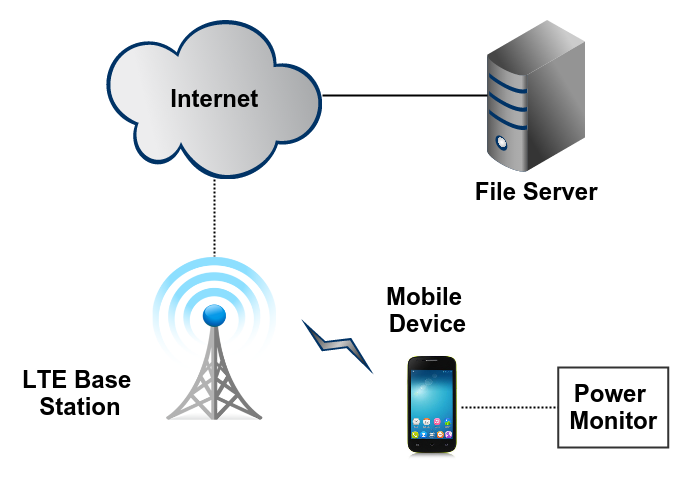
\includegraphics[width=0.7\textwidth]{images/cellular-test.png}
  \caption{The Experiment Setup for Cellular Transmission Tests}
  \label{fig:cellular-test}
\end{figure}

\begin{figure}[htbp]
  \centering
  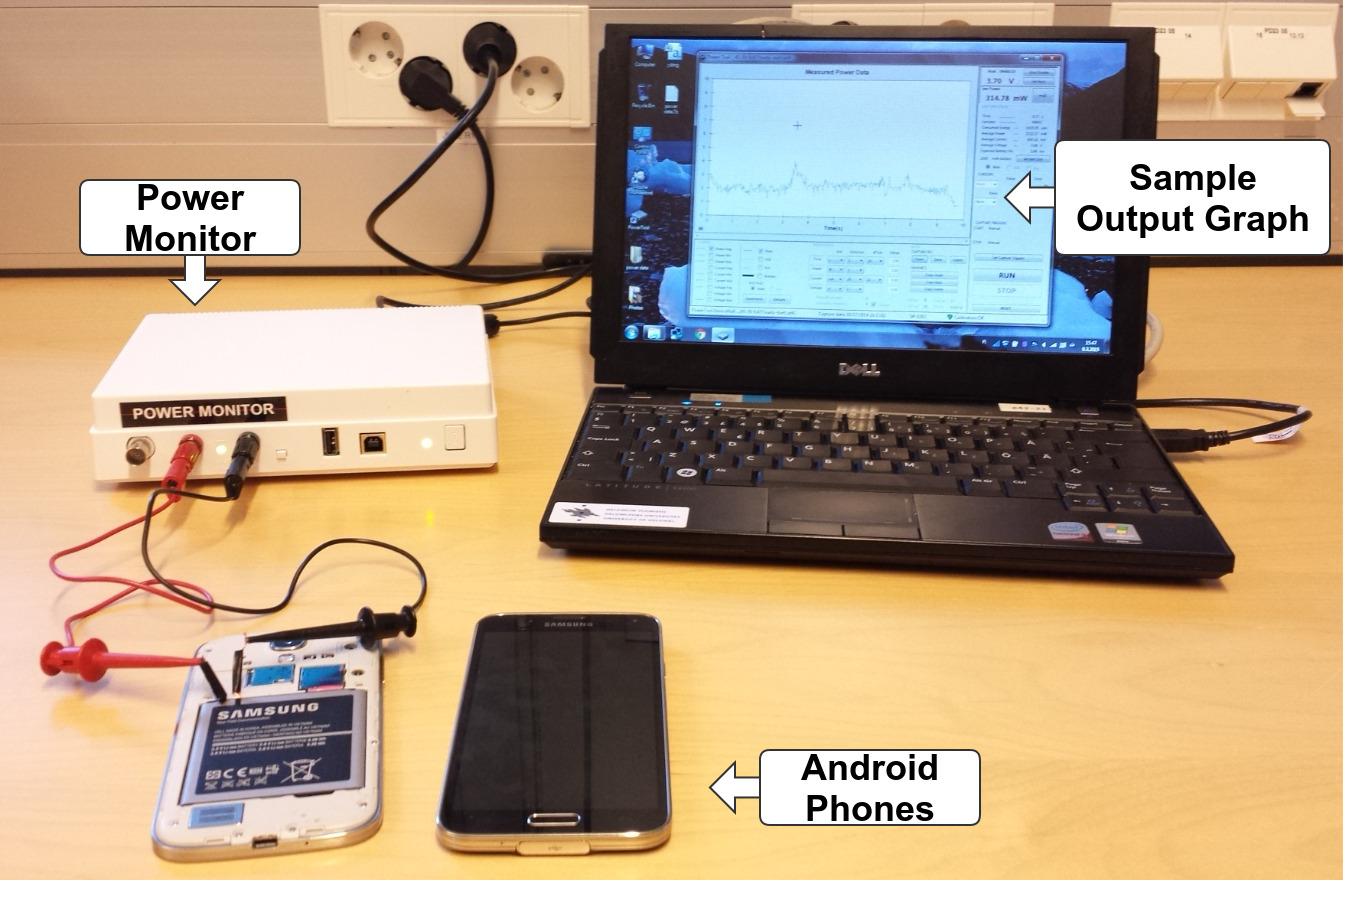
\includegraphics[width=0.7\textwidth]{images/power-monitor.jpg}
  \caption{Power Monitoring -- the power monitor, an opened mobile phone for energy measurements, and a sample output graph are shown in this photo.}
  \label{fig:power-monitor}
\end{figure}


To verify the practical transmission rate of an LTE network, we set up the following testbed shown in Figure \ref{fig:cellular-test}. We measure the time to download a fixed-size file from a server located in our department in Helsinki. Since we do not have any manageable LTE base station, we use the LTE service provided by a local cellular operator named DNA\footnote{DNA Oy. \url{https://www.dna.fi/}}. All experiments are performed on Android mobile phones with our own testing application, which executes a downloading task via HTTP connection to fetch a file (15 MB) from the server and records downloading times. We also collect energy data for file transmission in this test. To obtain fine-grained energy measurements, we use a high-precision digital power monitor\footnote{Monsoon Power Monitor. \url{https://www.msoon.com/LabEquipment/PowerMonitor/}} to collect test data as shown in Figure \ref{fig:power-monitor}. To measure the power drawn by mobile phones, we use the monitor instead of the battery to supply devices with power.


We choose the 4G subscription with the highest connection speed in DNA. The cellular operator declares that this subscription shall work at the maximum downstream speed of 150 Mbps, and an average speed between 5-80 Mbps. Our test results are shown in Table \ref{tab:cellular-speed}. As we can see, mobile phones achieve about 45 Mbps downstream speed in our 4G test environment, which is much faster than the average speed of 3G networks. Since the downloading time is reduced in 4G networks, average energy consumption for downloading files also drops on mobile phones. 

\begin{table}[htbp]
\centering
\begin{tabular}{|p{90pt}|p{60pt}|p{75pt}|p{60pt}|p{75pt}|}
  \hline
  & \multicolumn{2}{c|}{Galaxy S4} & \multicolumn{2}{c|}{Galaxy S5}\\
  \cline{2-5}
  & Average Throughput (Mbps) & Average Power Consumption (uAh/Mb) & Average Throughput (Mbps) & Average Power Consumption (uAh/Mb) \\
  \hline
  LTE (-76dBm\footnotemark[7]) & 45.47 & 4.54 & 42.12 & 4.06 \\
  \hline
  HSPA (-76dBm\footnotemark[7]) & 6.80 & 25.98 & 6.27 & 19.75 \\
  \hline
\end{tabular}
\caption{Measured Throughput and Energy Consumption on Mobile Phones in Cellular Networks}
\label{tab:cellular-speed}
\end{table}


\footnotetext[7]{With this received signal strength ($\geq -76dBm$), testing mobiles show full cellular signal bars (which means excellent signal level).}


\vspace{1mm}

\textbf{Measurement in WiFi environment}

\vspace{1mm}

\begin{figure}[htbp]
  \centering
  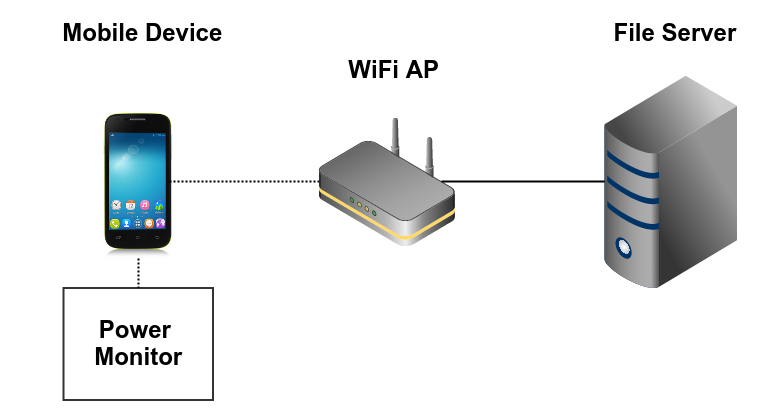
\includegraphics[width=0.7\textwidth]{images/wifi-test.png}
  \caption{The Experiment Setup for WiFi Transmission Tests}
  \label{fig:wifi-test}
\end{figure}

Testing results under LTE networks are helpful for us to have a sense about current practical transmission rates of cellular networks in Finland and Europe. However, people may still have this kind of questions: which type of network is faster? 4G or WiFi? In our test, LTE networks provide high downstream rates, how about current WiFi networks? To have better understanding on WiFi transmission speed, we set up the test bed shown in Figure \ref{fig:wifi-test}, and compare its testing results to the transmission rates in cellular networks we have obtained. In the following test, mobile phones are connected to the file server via a manageable WiFi AP (ASUS RT-AC68U) without any other middleboxes. We measure the transmission time and energy consumption on mobile phones with the same Android application, and the results are listed in Table \ref{tab:wifi-speed}.

\begin{table}[htbp]
\centering
\begin{tabular}{|p{110pt}|p{50pt}|p{75pt}|p{50pt}|p{75pt}|}
  \hline
  & \multicolumn{2}{c|}{Galaxy S4} & \multicolumn{2}{c|}{Galaxy S5}\\
  \cline{2-5}
  & Average Throughput (Mbps) & Average Power Consumption (uAh/Mb) & Average Throughput (Mbps) & Average Power Consumption (uAh/Mb) \\
  \hline
  802.11ac (-42dBm\footnotemark[8]) & 189.80 & 1.28 & 208.81 & 1.26 \\
  \hline
  802.11n (-42dBm\footnotemark[8]) & 43.62 & 4.17 & 111.53 & 1.89 \\
  \hline
\end{tabular}
\caption{Measured Throughput and Energy Consumption on Mobile Phones in WiFi Networks}
\label{tab:wifi-speed}
\end{table}


\footnotetext[8]{On this signal level, testing mobiles show full WiFi signal bars.}

Although 802.11n networks may have a theoretical maximum of 600 Mbps \cite{80211n}, and the newer 802.11ac standard offers an even higher transmission rate, the practical transmission rates are much lower due to real factors like distance, number of users and channel interference. As shown in Table \ref{tab:wifi-speed}, devices may achieve a 50 Mbps downstream rate (Galaxy S5 shows better performance in 802.11n mode with the same testing set-ups) in our 802.11n network, which is similar to the value in 4G networks. The practical throughput of 802.11ac is much higher than other types of networks. In our test environment, the average downstream throughput of 802.11ac is about 200 Mbps. With the increasing of transmission rates, data transferring in 802.11ac networks becomes more energy efficient.

\vspace{1mm}

\textbf{Insights}

\vspace{1mm}

Though we can not directly compare the transmission rates of WiFi and cellular networks obtained in our tests, the results still offer us some insights.

\begin{itemize}
  \item With the newer 802.11ac standard, WiFi networks may offer better transmission rates and energy-consumption properties even compared with current LTE networks. When building costs and manageable features are considered, WiFi networks as well as WiFi data offloading will still be great supplements for cellular networks presently and in the near future.
  \item LTE networks have provided good speed properties in file transferring. Though WiFi networks may show better bandwidth in some scenarios, it is not the time to simply yield that it is always beneficial to offload everything to WiFi networks. Unlike the cellular networks mentioned in \cite{bmv10}, currently LTE networks offer good link speed features, and may also be very energy-efficient. We shall consider both of the overhead and bandwidth factors carefully before making offloading decisions.
  \item In our test, the WiFi network shows impressively good performance, and one of the major reasons is that the testing AP is directly connecting to a local server without any middleboxes and potential traffic limitations. Like what addressed by MADNet \cite{dhx+13}, data pre-fetching and caching at WiFi APs may enhance file transferring and save more energy on mobile devices.
\end{itemize}


\subsubsection{Number of Accessible WiFi APs}

Some existing research work (e.g. \cite{dhx+13}) has already shown that open accessible WiFi APs in current networks are very limited. Most of the WiFi APs in an open environment require specific authentication like user-names and passwords. To verify this, we also conduct a simple field study in Helsinki. 

We design and implement an Android application (on Android 4.0+) for scanning and testing the accessibility of WiFi APs. It periodically scans neighboring WiFi APs and performs ping test to a public reference server for all open APs with 10-second intervals. It pops up specific messages on the screen when it starts and stops testing. We perform this experiments with Galaxy Tab 2 and Galaxy S4 at walking speed alone Aleksanterinkatu street, which is one of the most popular avenues in Helsinki. Once the scanning starts on the mobile devices, we stop and wait until it finishes, and then continue to walk until a new turn of scanning. We repeat tests on both sides of Aleksanterinkatu, and the walking tour is shown in Figure \ref{fig:map}.

\begin{figure}[htbp]
  \centering
  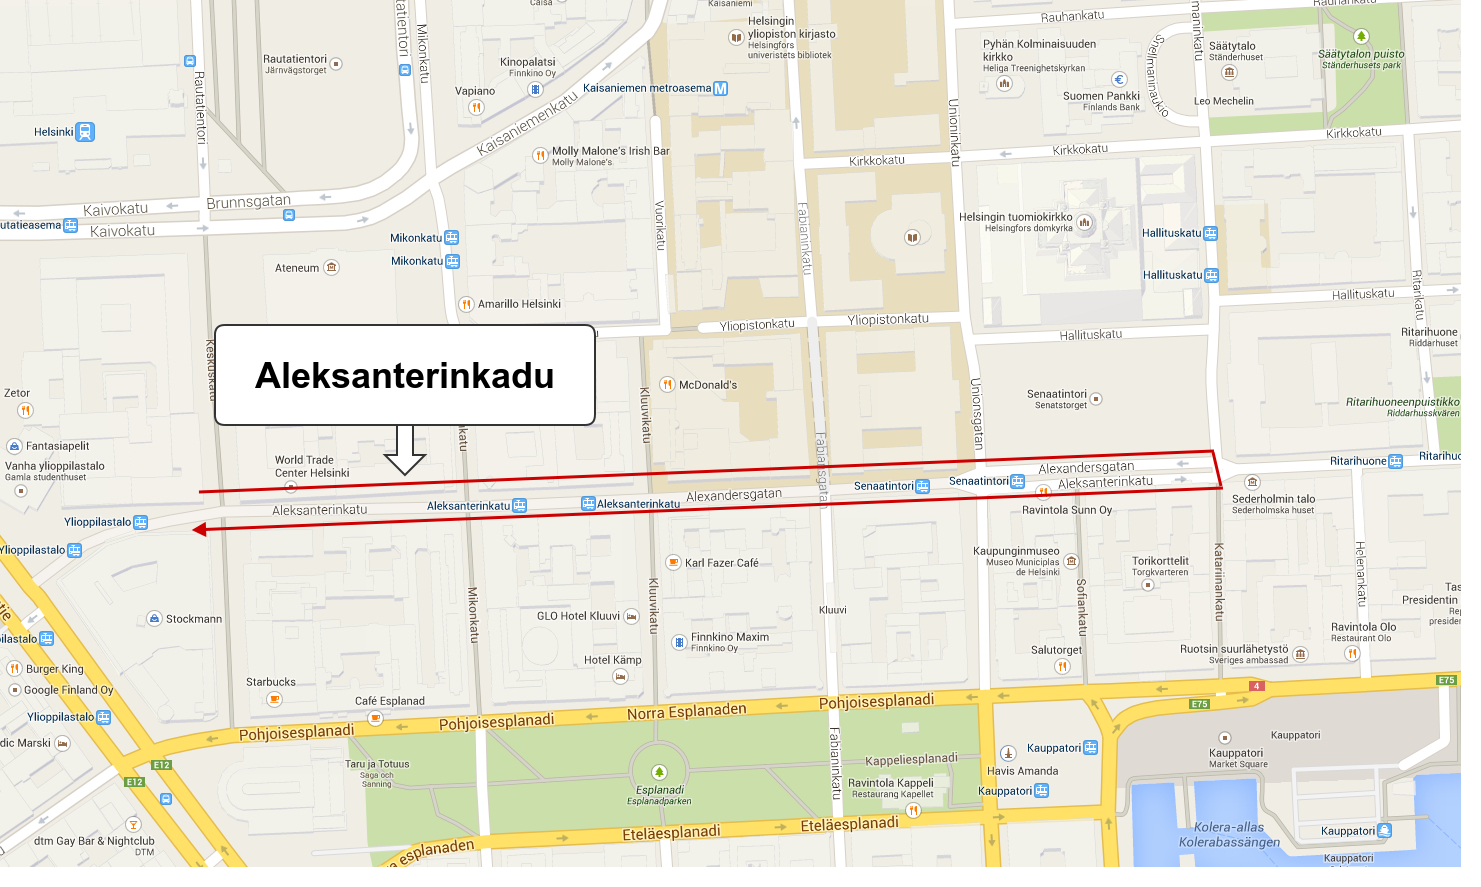
\includegraphics[width=0.95\textwidth]{images/map.png}
  \caption{Measurement on the Number of Accessible WiFi APs -- we take a walking tour along the Aleksanterinkatu street.}
  \label{fig:map}
\end{figure}

In our experiment, most of APs are not accessible, which shows a similar result to some existing research work. The result is shown in Table \ref{tab:stat-ap}. Among all the detected APs, about a quarter of them are open without encryption, but the percentage of really accessible APs is considerably low (1.5\%). Typically even an "open" AP requires extra authentication for data connection.

One thing to note here is that the number of accessible APs we got in the test may be inaccurate, and the real value is probably larger. Instead of specified account authentication, some open APs just require web-based activation without any password. Users can use those APs after they enable them with browsers, but our testing application fails to detect this. For example, in our experiment, a public WiFi network with ESSID 'Helsingin kaupungin WLAN' (27 different APs found with this ESSID) provides accessible connections if we activate it via its web page. However, those APs are considered as inaccessible ones in the test result.


\begin{table}[htbp]
\centering
\begin{tabular}{|c|c|c|}
  \hline
  Detected APs & Open APs without Encryption & Accessible APs \\
  \hline
  877 & 220 (25\%) & 13 (1.5\%)\footnotemark[9] \\
  \hline
\end{tabular}
\caption{Statistics of WiFi APs in Helsinki}
\label{tab:stat-ap}
\end{table}

Although there may be some measurement errors on the number of accessible APs, our test result still shows an obvious phenomenon that accessible APs are much less than the total detected APs. Only about 25 percent of APs in our test are open, and the percentage of accessible APs is definitely lower than that. If offloading can be only perform on open APs, it will be quite challenging due to the limited percentage of accessible APs. To really enable traffic offloading, cellular operators shall consider to provide more collaborative WiFi APs as supplements to their cellular networks. \footnotetext[9]{Due to the implementation of our test application, there may be some measurement errors here, and the real number may be larger than this one.}



\subsubsection{Signal Level and Its Influences on Data Transmission}

As we know, the lower the received signal strength of a mobile device is, the worse connection rate the device gets over a WiFi network. To test how bad the transmission rate drops when a device gets far away from a WIFi AP, and gain practical experience on the relationship between signal levels and data transmission rates, we conduct the following experiment.

We set up a laptop (DELL E4200) with a 802.11n USB WiFi adapter (NETGEAR WNA1100) running hostapd\footnote[10]{hostapd, \url{http://w1.fi/hostapd/}} to act as a WiFi access point, and run Apache2 on the laptop as a file server. Then we connect multiple Android mobile phones (Samsung Nexus S, Samsung Galaxy S2, Samsung Galaxy S3, Samsung Galaxy S4, Samsung Galaxy S5) to this AP respectively, and perform downloading tests from the Apache2 server with different distances to the AP, as well as record the energy consumption and downloading time for each turn. Figure \ref{fig:signal-level-topo} shows the basic topology of our test.

\begin{figure}[htbp]
  \centering
  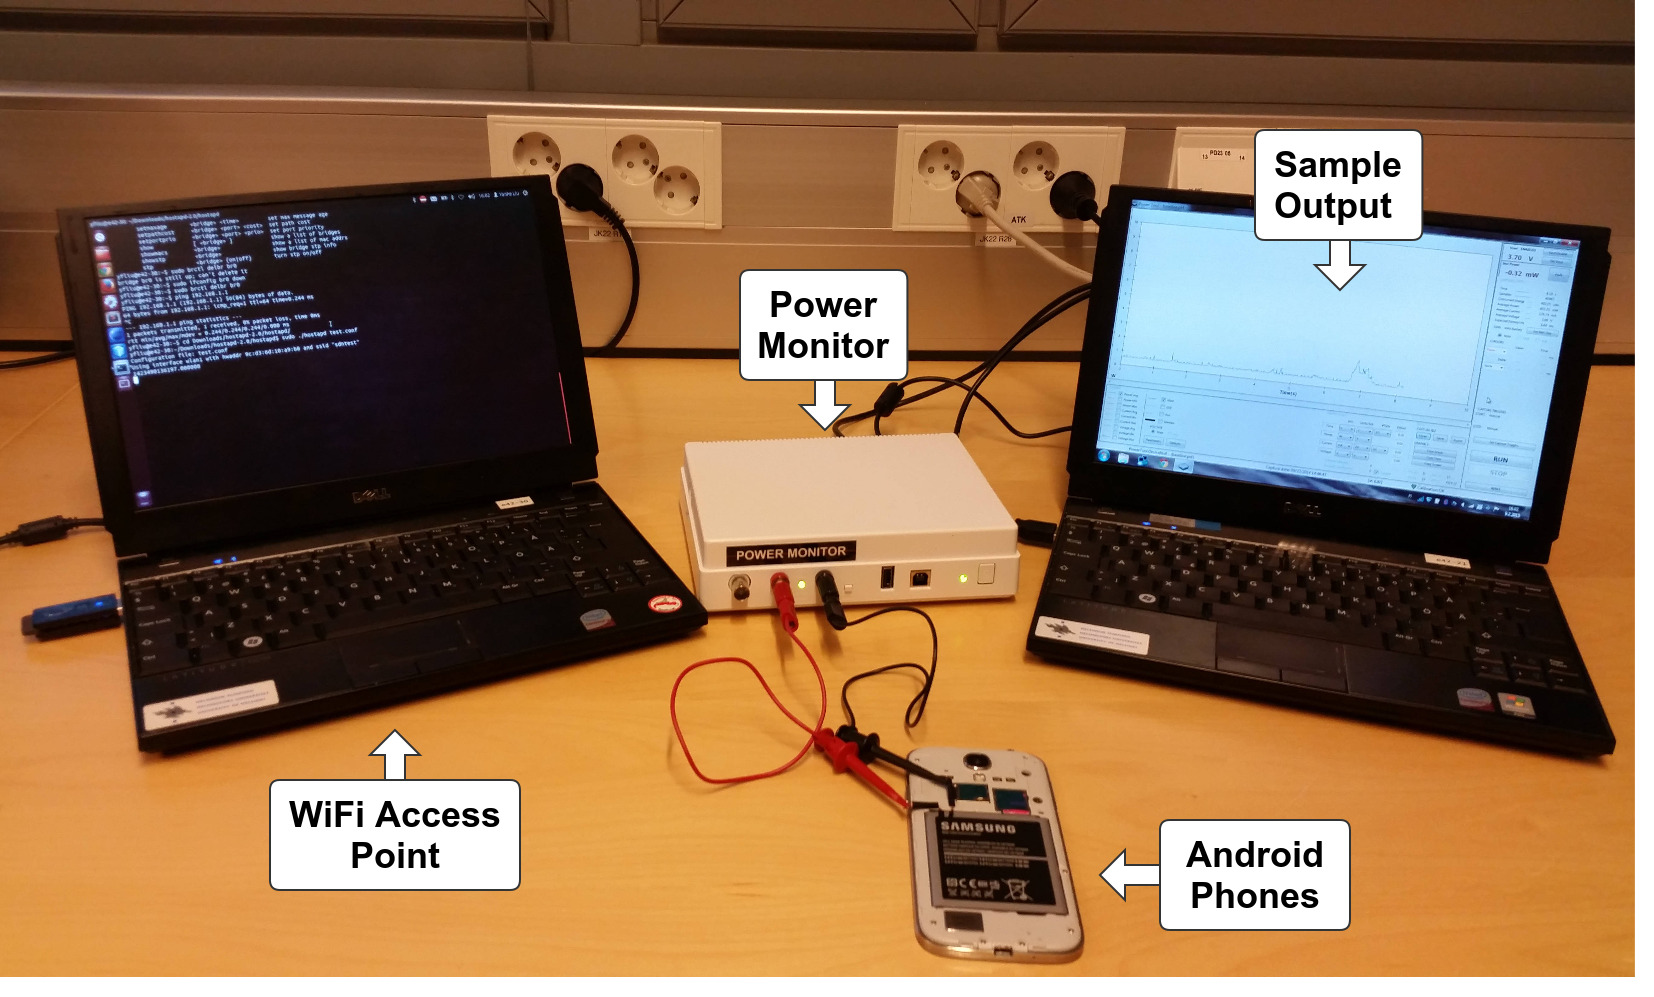
\includegraphics[width=0.8\textwidth]{images/signal-level-topo.jpg}
  \caption{The power monitor, an opened mobile phone for energy measurements, a laptop with a USB WiFi adaptor acting as a WiFi access point, and a sample output graph are shown.}
  \label{fig:signal-level-topo}
\end{figure}

The experiments are also performed on Android phones with our own downloading application which is used for the previous LTE downloading test. Mobiles fetch a fixed-size file (33.66 MB) from the server via HTTP connection, and records downloading times and received signal levels from the devices. We took the whole setup out in our office at the University of Helsinki, and ran the test at a number of different distances. The test results are shown in the Figure \ref{fig:signal-level}, and we measure the received signal strength in dBm. In Figure \ref{fig:signal-level-time}, the relationship between the signal level (distance) and the average transmission time is displayed, and Figure \ref{fig:signal-level-power} illustrates the relation of the signal level to the power consumption. 

\begin{figure}[htbp]
  \centering
  \subfloat[Signal Level and Transmission Time]{
    \label{fig:signal-level-time}
    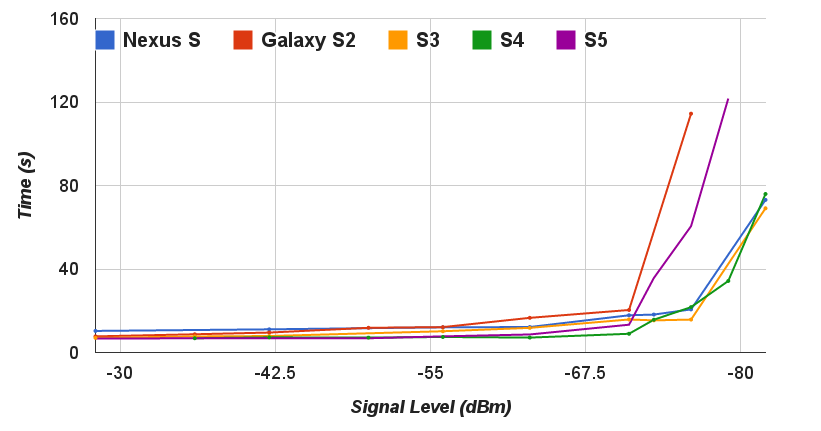
\includegraphics[width=0.8\textwidth]{images/signal-level-time.png}
  }
  \hspace{5pt}%
  \subfloat[Signal Level and Power Consumption]{
    \label{fig:signal-level-power}
    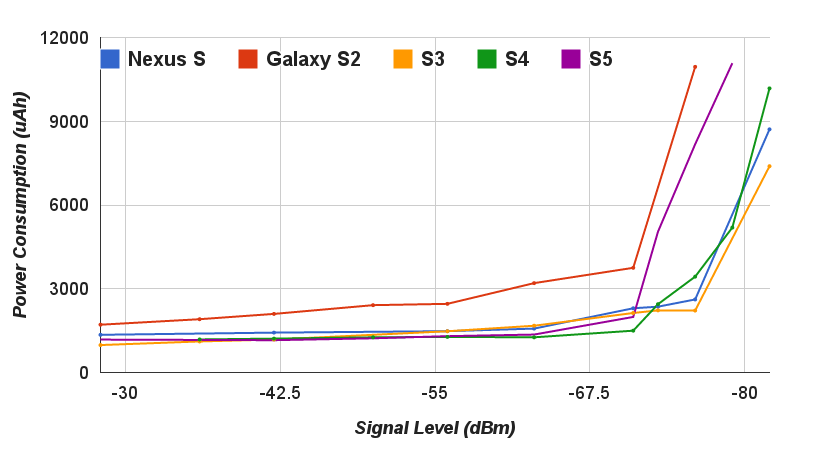
\includegraphics[width=0.8\textwidth]{images/signal-level-power.png}
  }
  \caption{Signal Level and Its Influences on Transmission Time/Power in 802.11n Networks}
  \label{fig:signal-level}
\end{figure}

When the received signal level is higher above -60dBm (typically means the signal level is "strong"), the average transferring rate does not change much on different devices, and the average throughput is close to the maximum value of our AP. However, when the signal strength drops below -70dBm, transmission rate decreases sharply, and the energy consumption raises precipitously by several times. When it is below -80dBm, the downloading is almost "stopped" on all the devices and we can hardly finish downloading a 33MB file in 5 minutes. Furthermore, the power consumption and the transmission time show similar trends when the distance between the mobile device and the WiFi AP increases. In general, the longer the transmission time is, more power a mobile device consumes. The power consumption is always directly proportional to the total transmission time.

\vspace{1mm}

\textbf{Insights}

\vspace{1mm}

The signal level data shows that our system shall select WiFi AP carefully for offloading. If a "wrong" (with poor signal level) AP is chosen, mobile devices may suffer from worse data transfer performance and more energy consumption. Based on our test result, we generate a mathematical signal level model and use it in our offloading system for make switching decisions. This model is explained in the design section.


\subsubsection{Client Competition Interference on One WiFi AP}

The next experiment is driven from a real scenario: when multiple users are gathering together and connect to the same AP, do they affect each other? How does an individual device perform on data transmission with others? How about the overall throughput of that AP?

We design the following test to verify the influence of adding multiple users on one WiFi AP. The general idea of this experiment is quite simple: we first measure the time for downloading a fixed-size file with one mobile device via our testing AP. Then we add another device, and try to use these two devices together to transfer data, as well as record individual and overall throughput again.

\textbf{Experimental Setup}: it is similar to what we use in the signal level test. We set up a laptop (DELL E4200) to act as a WiFi access point with a 802.11n USB WiFi adapter (NETGEAR WNA1100), and run Apache2 on it as our testing file server. We first perform the test with our Android application on one Galaxy tab (Samsung Galaxy Tab 2, GT-P3100). The device is connected to the WiFi AP, and downloads a 33MB file from the server. Then we execute the downloading tests with two Galaxy tabs, place them with similar distances to the AP, and try to run them simultaneously (we start the downloading test manually on both of the devices, so there is a certain amount of error on starting time). The Table \ref{tab:competition} shows results of our test. Instead of simply adding throughput values of two tabs, we calculate the overall throughput by estimating the total transmission time for two devices. If there is only one device, the overall throughput is the same as individual throughput. As shown in Table \ref{tab:competition}, when a new device is added to the same AP, the overall throughput does not improve much (increase by about 5\%), but the individual performance for each device drops a lot (45\%). In our test, it almost shrinks to half since two competitors are exactly the same type of devices. In a word, adding new users on one WiFi AP may hurt everyone without enhancing overall performance.

\begin{table}
  \centering
  \begin{tabular}{|p{40pt}|p{110pt}|p{110pt}|p{105pt}|}
    \hline
    \textbf{Type} & \textbf{Avg Throughput of Tab 1 (Mbps)} & \textbf{Avg Throughput of Tab 2 (Mbps)} & \textbf{Overall Throughput (Mbps)} \\    
    \hline
    1 tab & 30.38 & / & 30.38 \\
    \hline
    2 tabs & 16.46 & 16.28 & 31.95 \\
    \hline
  \end{tabular}
  \caption{Downloading Competition Test on One WiFi AP}
  \label{tab:competition}
\end{table}

In addition, we conduct a simple test to verify the downloading performance of our Apache server with wired connection. It shows that our file server can easily offer a reading speed more than 700 Mbps via an 1Gb Ethernet port, which is much higher than the transmission rate obtained by mobile devices. The throughput values in Table \ref{tab:competition} are mainly limited by the wireless connection. 

Different from the above experiment, there may be rate limiting policies for different users on APs or access switches in real scenarios. How do devices perform if we set up bandwidth limitations on the testing AP? Do they still affect each other like the way shown in Table \ref{tab:competition}? To testify competition influences with rate limiting, we repeat our experiment by adding traffic shaping policies on our testing AP. 

We use Linux "tc" (traffic control) command to set up rate limiting policies for users based on their IP addresses, and the results are listed in Table \ref{tab:competition-tc}. As shown in the table, when the sum of individual bandwidth is lower than the total one of that AP, influences caused by competition of multiple users can be nearly ignored. However, if the individual bandwidth  increases, users start to affect each other when the total throughput gets close to the maximum value of the AP. In our test, the AP's maximum transmission throughput is about 32 Mbps. If we limit the bandwidth to 8 Mbps for each user, the two tabs do not affect each other when downloading the file at the same time. When we increase the limitation to 20 Mbps per user, the overall throughput of two tabs downloading together will be constrained by our AP's maximum bandwidth, and the two devices start to interfere each other. If the limitation increases to 24 Mbps, interference becomes more serious. The transferring performance of each device drops by approximately 30\% when two tabs are downloading together with the 24 Mbps bandwidth limitation. 

\begin{table}
  \centering
  \begin{tabular}{|p{45pt}|p{35pt}|p{90pt}|p{90pt}|p{95pt}|}
    \hline
    \textbf{Policy} & \textbf{Type} & \textbf{Avg Throughput of Tab 1 (Mbps)} & \textbf{Avg Throughput of Tab 2 (Mbps)} & \textbf{Overall Throughput (Mbps)} \\    
    \hline
    \multirow{2}{45pt}{8Mbps per-user} & 1 tab & 7.78 & / & 7.78 \\
    \cline{2-5}
    & 2 tabs & 7.78 & 7.78 & 15.57 \\
    \hline
    \multirow{2}{45pt}{20Mbps per-user} & 1 tab & 19.06 & / & 19.06 \\
    \cline{2-5}
    & 2 tabs & 17.43 & 16.57 & 32.99 \\
    \hline
    \multirow{2}{45pt}{24Mbps per-user} & 1 tab & 22.60 & / & 22.60 \\
    \cline{2-5}
    & 2 tabs & 14.69 & 15.49 & 29.104 \\
    \hline
  \end{tabular}
  \caption{Downloading Competition Test on One WiFi AP with Rate Limiting}
  \label{tab:competition-tc}
\end{table}

\vspace{1mm}

\textbf{Insights}

\vspace{1mm}

According to these test results, it is easily realized that multiple users may affect each other when they transfer data simultaneously on the same WiFi AP due to signal interference and forwarding congestion, and we shall consider this factor and the number of active AP users carefully for mobile offloading.


\subsubsection{Summary of Measurement Study}

Our measurement results well answer the questions we ask in the beginning of this section: 

\begin{itemize}
  \item WiFi-based mobile offloading is still a good and economical supplement to current 4G networks. 802.11 technologies are providing higher and higher transmission bandwidth, just like cellular ones. However, it may not be beneficial to always offloading data to WiFi networks, since cellular networks may show better performance in some scenarios.
  \item When we choose a "bad" AP for offloading, e.g. the AP is too far away, devices may suffer from extreme performance dropping and serious energy overhead. We have to consider various factors like signal levels, number of users, and bandwidth together to make a context-based offloading decision.
\end{itemize}


\subsection{Offloading Design}


\subsubsection{Design Objectives}

To address real-world challenges on traffic offloading, we put forth following requirements in our system design. In our opinion, a good traffic offloading scheme is not just about decision making on the side of cellular operators. It shall bring benefits to cellular operators, WiFi providers and mobile users.

\vspace{1mm}

\textbf{Throughput-Aware Offloading Decisions}

\vspace{1mm}

This system shall avoid naive traffic offloading, and make offloading decisions based on mobile throughput and system overall traffic loads. As we have seen from our measurement, mobile devices may suffer from worse throughput when an AP with poor signal strength is chosen. Instead of directly offloading data to different access points, this system shall offload data with the aim of increasing transmission throughput and balancing system loads. To achieve this, it needs to obtain information both on system traffic and client locations.

\vspace{1mm}

\textbf{Collaborative Management between Cellular and WiFi Accesses}

\vspace{1mm}

Some existing research studies \cite{dhx+13} and our measurement show that open accessible WiFi APs are very limited currently. Most of the time, WiFi APs require specific user-names and passwords for association. It is infeasible to just offload cellular traffic to WiFi APs without considering whether they are truly accessible for different users. A collaborative management system between cellular and WiFi access points is quite necessary for practical offloading.

Nowadays, WiFi access networks are considered as one integral part in the 5G architecture. This provides a great opportunity for traffic offloading since all the cellular and WiFi access points can be controlled in one system with the same authentication and billing mechanisms. However, it requires collaborative management between both kinds of access technologies. In our system, cellular and WiFi access points shall be controlled together in a consistent way.

\vspace{1mm}

\textbf{Practicality}

\vspace{1mm}

This system shall be practically implemented and easily deployed. A light-weight system designed for current 3G/4G networks without requiring extra modification on previous standards is preferred. We opt to achieve this through an overlay framework on existing cellular and wireless networks.


\vspace{1mm}

\textbf{Extensibility}

\vspace{1mm}

Though this system is mainly designed for traffic offloading at this stage, it shall be extensible for some different purposes. We hope to have an extensible framework which can be used for different types of wireless and cellular experiments later. To achieve this, we opt to build our system based on a software-based way, where diverse services can be implemented as software plug-ins on the top of the system.


\subsubsection{System Design Principles and Architecture}

Our system runs in a collaborative wireless network where one or several WiFi APs are deployed within the coverage of each cell. As shown in Figure \ref{fig:networks}, one cellular base station and WiFi APs are working together to provide network accesses to mobile users in one area, and some users may have options to connect to multiple different access points (both WiFi and cellular). In addition to the coverage overlap among cell base stations and WiFi APs, this system also handles re-association WiFi load balancing due to the coverage overlap of WiFi APs.

\begin{figure}[htbp]
  \centering
  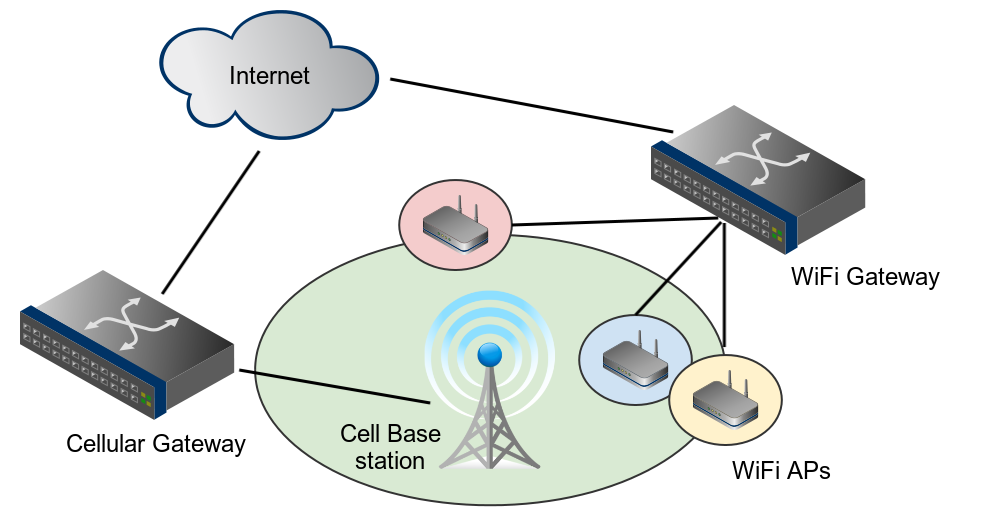
\includegraphics[width=0.7\textwidth]{images/networks.png}
  \caption{Basic Architecture of Current Cellular Networks -- in each cell, there may be one or more WiFi APs deployed besides the cell base station.}
  \label{fig:networks}
\end{figure}

As we reviewed in Chapter 2, some existing work has already tried to use a centralized controller to manage client behaviors and network assignments in a collaborative network. We are going further in this direction with more simplified programming models and better practicality. Inspired by the work of Odin \cite{sszm+12}, we choose to develop a platform in an SDN approach. Current SDN structures and techniques provide great programming modularity, traffic monitoring solutions, and excellent extensibility. 

\begin{figure}[htbp]
  \centering
  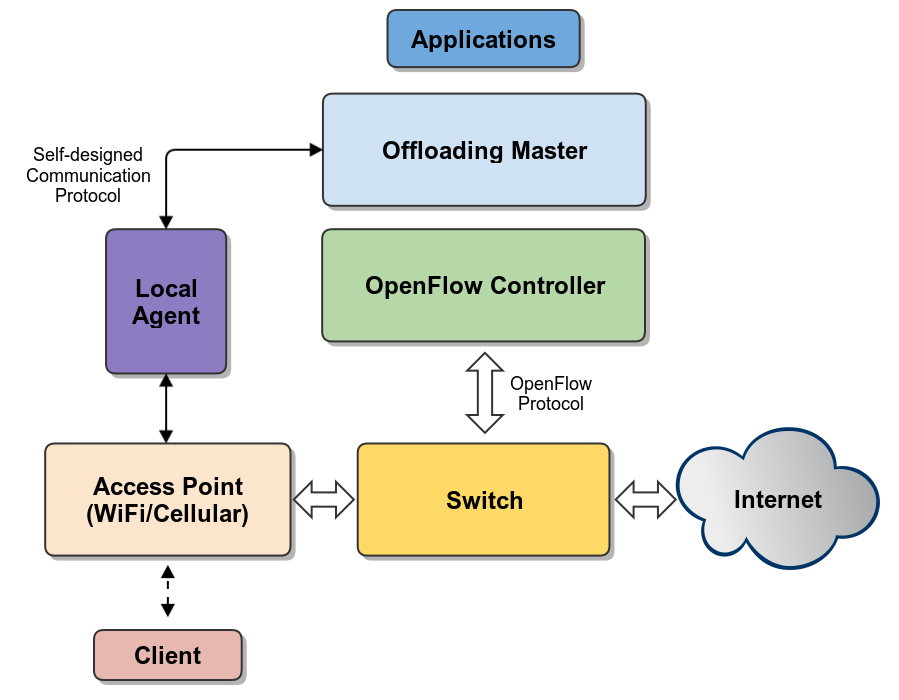
\includegraphics[width=0.7\textwidth]{images/architecture.png}
  \caption{Architecture of Our Platform -- the offloading master runs as an application on the top of an OpenFlow controller, and speaks to each local agent running on APs (base stations) with a custom protocol.}
  \label{fig:architecture}
\end{figure}

Our platform comprises four major components: a centralized offloading controller, several local agents, client-side extensions, and OpenFlow-enabled devices. Its architecture is shown in Figure \ref{fig:architecture}. The offloading master runs on an OpenFlow controller as an application to make offloading decisions. We implement our traffic management logic in this master module. The underlying OpenFlow controller provides a global view over the network topology, and thanks to the monitoring features of OpenFlow, the offloading master can be quickly aware of traffic flows in the network. Since OpenFlow protocol is only used for flow traffic management, we design our own local agent for wireless association and client monitoring. It runs on wireless APs (or cellular base stations), and also offers communication channels between clients and the offloading master.

To utilize client-side measurement, a client module is added into mobile devices. By exploring the rich context offered by clients in this way, our platform can provide the central controller with better visibility on networks and more management possibilities. The client module does not change current existing wireless and cellular standards, but only introduces enhanced functionality for offloading and measurement. It can be used to solve problems which are difficult with AP-only observations, like location detection and awareness of running applications on client devices.

In addition, this platform can be easily extended by adding new applications on the top of Offloading or OpenFlow controller. Different offloading configurations and policies for various scenarios can also be added into this platform.

\subsubsection{Communication Protocol Design}

To coordinate several independent components (a central controller, local agents, and clients), we design and set up two communication channels in our system. As shown in Figure \ref{fig:communication}, there is a \textbf{Controller Channel} between the central controller and the local agent, and a \textbf{Client Channel} between the agent and the client module.

\begin{figure}[htbp]
  \centering
  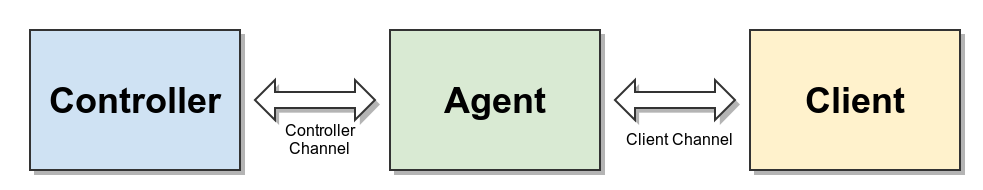
\includegraphics[width=0.9\textwidth]{images/communication.png}
  \caption{Two Communication Channels in Our System -- Controller Channel and Client Channel}
  \label{fig:communication}
\end{figure}

The central controller and agents use the Controller Channel for communication. The controller sends management requests to agents and invokes commands on agents. Local agents also send out messages to the central controller for reporting network events. For example, when an agent detects a new client, it sends messages to the controller to report this event.

To enable client management and client-side data collection, there is another communication channel between the client module and the agent. Instead of creating a direct channel between the controller and each client, we take agents as proxies in communication. When a client tries to send messages to the central controller, it first transmits those messages to the agent which it is connecting to, and then the agent forwards those messages to the controller via the Controller Channel. Similarly, the controller also uses the agent as a proxy to send requests to clients. As shown in Figure \ref{fig:communication}, clients can not directly communicate with the controller, but only with its local agent. In this way, the central controller is not directly exposed to clients. By blocking some unrelated packets on the agent side, we may increase the security of the whole system, and reduce the traffic load on the controller side.

To support this kind of communication, we design a custom protocol. It shall not only help the controller to recognize what type a packet belongs to, but also tell the agent what the destination of a frame is. In our protocol, several bytes are used to indicate what a packet is used for, and where it shall be delivered to. For example, if the controller tries to send a frame to a client, there are some bytes to indicate this for the agent, and the client address is also included for further transmission.

\subsubsection{Offloading Decision Making}

In this part, we focus on offloading decision making, illustrate it as an optimization problem, and explain our basic idea on collaborative network re-assignment. Instead of making offloading decision naively, our system shall take several practical factors (like signal strength, potential bandwidth, and user mobility) as input, and then computes the appropriate offloading interfaces (specific WiFi APs or cellular base stations) in a mathematical way. In general, it shall answer the following questions: When shall the offloading happen? Which clients shall be moved to different networks? Where shall the traffic be offloaded?

\begin{algorithm}
\caption{Offloading Algorithm}
\label{alg:offloading}
\begin{algorithmic}[1]
\Procedure{OffloadingProcedure}{}
  \State \uppercase{INPUT:} $W$ is the set of access points and access switches
  \State \uppercase{INPUT:} $totalBandwidth_i$ is the total bandwidth of a given node $i$
  \State \uppercase{INPUT:} $currentBandwidth_i$ is the current real-time bandwidth of a given node $i$
  \State \uppercase{INPUT:} $k$ is a constant coefficient
  \While {TRUE}
    \For {${w}\in{W}$} 
      \State \textit{\textbf{Traffic Load Detection}} on $w$
      \If {$currentLoad_w \geq k \cdot maxBandwidth_w$}
        \State $C \gets \textit{\textbf{Choose Offloading Client Set} on w}$
        \For {${c}\in{C}$}
          \State \textit{\textbf{Choose Offloading Destinations}} for $c$
        \EndFor
      \EndIf
    \EndFor
    \State \textit{Wait for Detection Interval v}
  \EndWhile
\EndProcedure
\end{algorithmic}
\end{algorithm}

\begin{figure}[htbp]
  \centering
  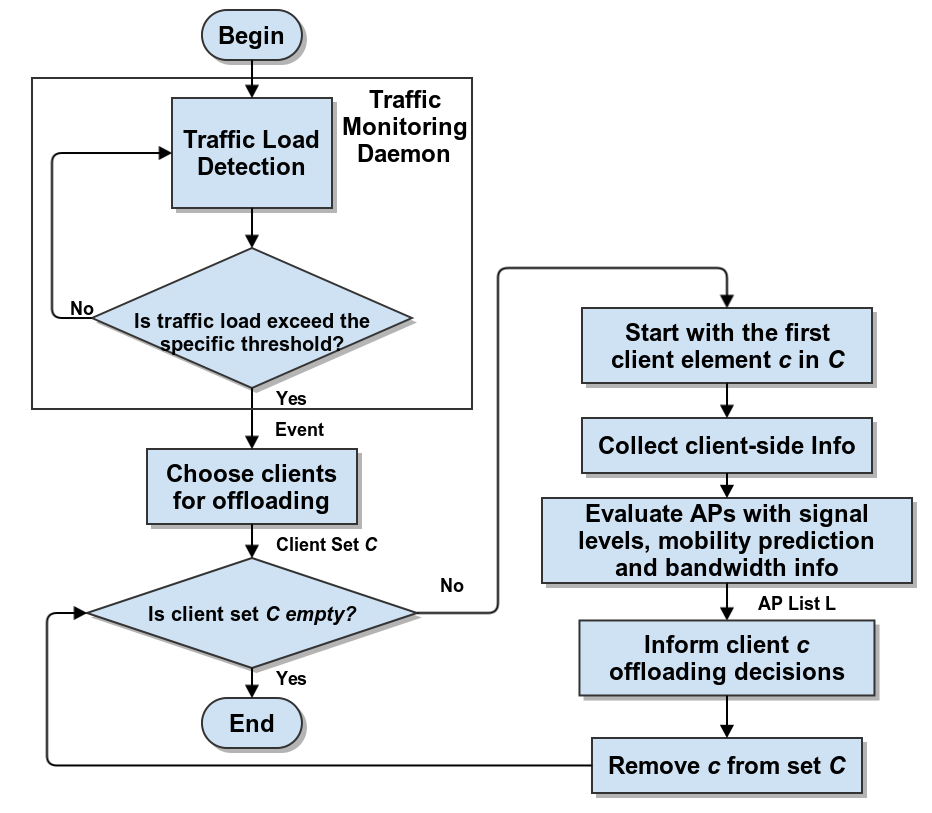
\includegraphics[width=0.8\textwidth]{images/algorithm.png}
  \caption{Offloading Algorithm}
  \label{fig:algorithm}
\end{figure}


We describe its basic steps in Algorithm \ref{alg:offloading}. The outer "while(true)" loop means this algorithm continuously runs as a separated process in the background (typically like a daemon process). A monitoring module performs "load detection" on each access point and access switch controlled by our system. If the current traffic load reaches a certain threshold several times consecutively on a node, offloading on this node is triggered. In Algorithm \ref{alg:offloading}, we use $k \cdot maxBandwidth_w$ as the traffic threshold of node $w$, where $k$ is a constant coefficient (e.g. 0.7). When offloading is requested on a specific node, decision-making module first chooses client candidates connecting to this node for potential offloading, and evaluates offloading destinations for each candidate. If possible, the system tries to select the most beneficial offloading destination for the client candidate, and inform it to switch. In Figure \ref{fig:algorithm}, each step is shown in a flow chart. The system shall perform WiFi-based mobile data offloading (or load balance) only when it may bring benefits to both mobile users and the networking system.

In our algorithm, there are several key design points, like "choosing offloading clients" and "destination selection". We explain each of them respectively as follows:

\begin{enumerate}
\item \textbf{Load Detection and Client Choosing}

Here we put \textbf{load detection} and \textbf{client choosing} together, because these two components always cooperate together. In general, load detection is performed by a monitoring process with specific thresholds. If the total traffic load exceeds a certain threshold on an access node for a while, and there are multiple active clients connecting to this node, offloading will be triggered. 

When there is no rate limitation policy on any mobile client, the load detection and client choosing work in a simple way: we set the threshold with a high value (e.g., $0.7 \cdot maxBandwidth$). If this threshold is reached, we think that the bandwidth utilization ratio is too high, and users may interfere each other and suffer from bad throughput. The mobile clients with top bandwidth utilization ratios are considered as offloading candidates.

When there are traffic shaping policies on mobile clients, this threshold shall be set with a lower value (e.g., $0.5 \cdot maxBandwidth$). In this case, each client may only take a small part of the total bandwidth. If we still use a high threshold, we may have to ask dozens of clients to move at the same time for reducing the bandwidth utilization, which may be inefficient and error-prone. For avoiding this kind of problems, we choose to trigger offloading earlier. Instead of choosing the mobile clients which are consuming more bandwidth, those inactive users who have connected for a long time are preferred to leave.

\item \textbf{Evaluating Offloading Destinations}
To make beneficial offloading decisions, the system may have to collect various information both from the user side and the system side. The OpenFlow controller and local agents are natural choices for obtaining system information on bandwidth utilization and client numbers. Since there is a client-side extension, we can also easily gain information from the client side.
  
As we mentioned in the measurement study, good signal strength is important for data transmission. So the master first tries to collect received signal information from the candidate clients, and make mobility prediction for them based on their signal records when offloading is triggered. Then, the system evaluates available access points based on bandwidth utilization ratios and signal information. Based on our previous measurement study, we formulate a mathematical model to compare different factors and evaluate the potential AP performance. For a client $c$ which is now connecting to the AP $w$, the mathematical evaluation metric for a specific offloading destination AP $a$ is shown like this:
  
\begin{equation} \label{eq:offloading}
  c_0 \cdot \mu \cdot (1 - e^{-k_0(S - k_1)}) \cdot  \frac{estimatedB_a}{\operatorname*{arg\,max}_a estimatedB_a} \cdot \frac{restB_a}{totalB_a} - c_1 \cdot \mathbbm{1}{w}
\end{equation}

In this model, we use $c_0 \cdot \mu \cdot (1 - e^{-k_0(S - k_1)}) \cdot  \frac{estimatedB_a}{\operatorname*{arg\,max}_a estimatedB_a} \cdot \frac{restB_a}{totalB_a}$ to estimate and evaluate client's potential throughput on node $a$, and $c_1 \cdot \mathbbm{1}{w}$ to measure offloading overhead. Since there are several different groups of parameters in this metric, we explain our model separately.


\begin{itemize}
  \item $c_0, c_1$ are constant weight parameters in the polynomial. Different weight combinations show dissimilar preferences on throughput and offloading overhead. For example, a larger $c_1$ means overhead have more negative effects on making offloading decisions.

  \item $\mu \cdot (1 - e^{-k_0(S - k_1)})$ shows influences of signal levels and potential mobility on future throughput. $\mu(0<\mu\leq 1)$ is a mobility prediction parameter. The further the client $c$ is predicted to leave from $a$, the smaller this parameter is.

As shown in Figure \ref{fig:signal-level}, transmission throughput drops steeply when the received signal level decreases below a threshold value (approximately -73dBm in our experiment). Based on our measurement results, we formulate an exponential metric $- e^{-k_0(S - k_1)}$ to measure this effect, where $S$ is the received signal level of node $a$ seen from the client $c$ in dBm. Both of $k_0$ and $k_1$ are constant parameters to scale and adjust this exponential metric. $k_1$ numerically equals to the signal level at which the throughput on this AP starts to decrease sharply. We draw this exponential metric in Figure \ref{fig:model} with $k_0 = \frac{1}{3}$, and $k_1 = -73$.
  
\begin{figure}[htbp]
  \centering
  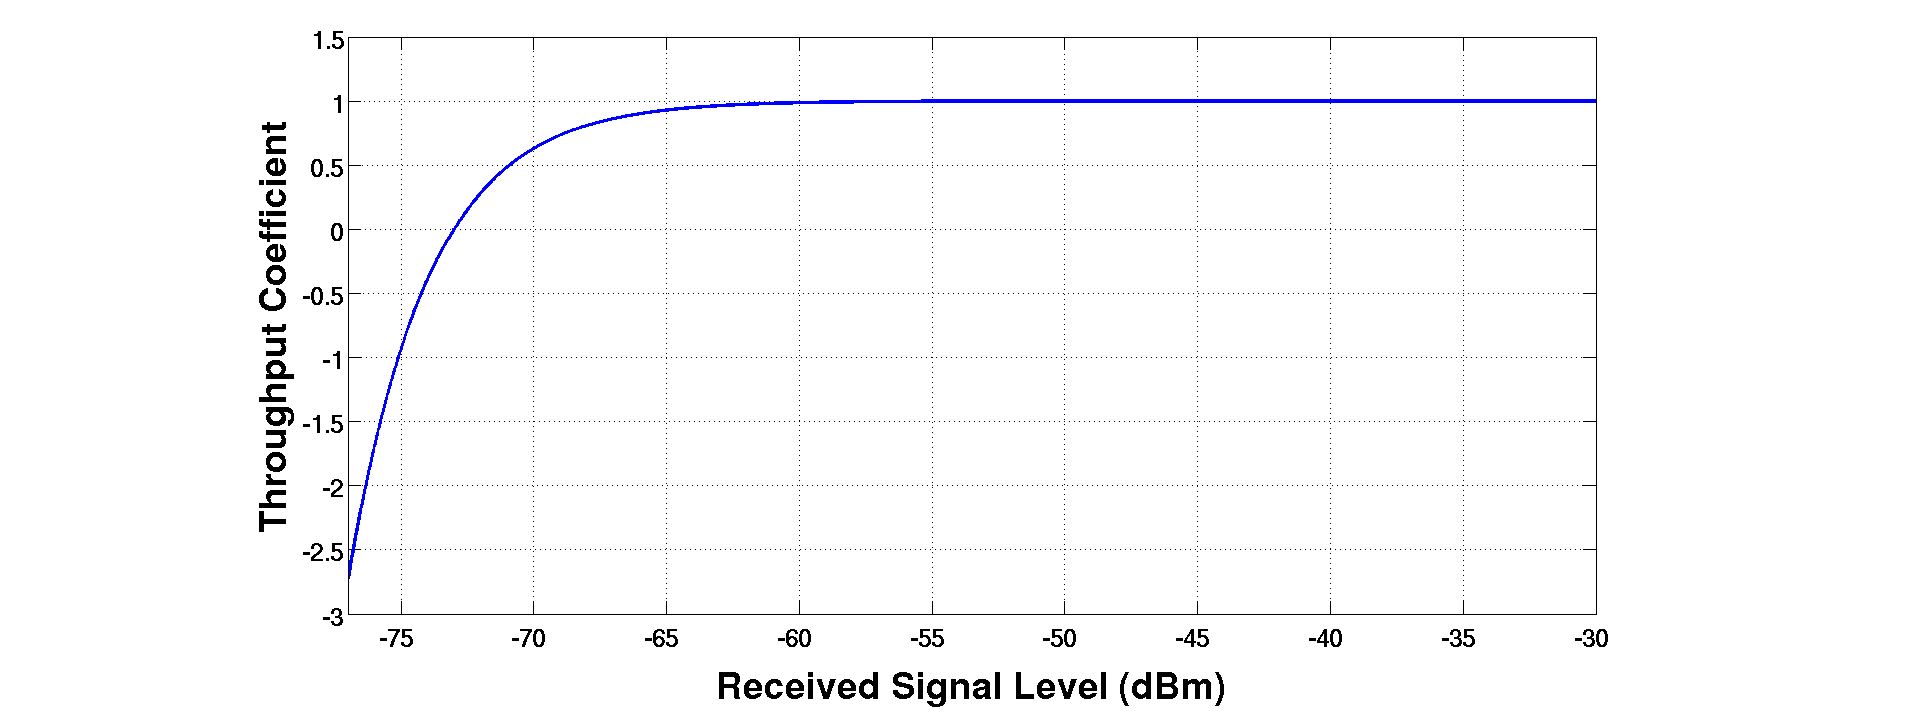
\includegraphics[width=0.85\textwidth]{images/model.png}
  \caption{Evaluation Metric for Signal Levels ($k_0 = \frac{1}{3}$, and $k_1 = -73$)}
  \label{fig:model}
\end{figure}  
  
In our measurement, the transmission throughput exponentially drops when the received signal level on a mobile device is below -73dBm in 802.11n WiFi APs. As we can see, our exponential metric exactly shows the same decreasing feature as the power consumption and the downloading time illustrated in Figure \ref{fig:signal-level}.
  
  \item $estimatedB_a$ is the estimated bandwidth on node $a$ for the client $c$, and $\operatorname*{arg\,max}_a estimatedB_a$ is the maximum value among all the estimated bandwidth values of candidate APs. $restB_a$ is the rest idle bandwidth on node $a$, and $totalB_a$ is this node's total bandwidth. $\frac{restB_a}{totalB_a}$ shows the bandwidth utilization ratio for node $a$, and $\frac{estimatedB_a}{\operatorname*{arg\,max}}$ ranks candidate APs based on absolute bandwidth configuration.
  
  \vspace{5mm}
  
  In general, we estimate client throughput on each different AP by combining bandwidth and signal factors together. As we have shown in the measurement study, client real throughput is not only affected by bandwidth situations, but also influenced by distances and signal levels.
  
  \item $\mathbbm{1}{w}$ is an indicator function for node $a$:

$$ \mathbbm{1}{w}(a)=\begin{cases}
0,\quad a = w \ (a \ and \ w \ are \ the \ same \ AP) \\
1,\quad a \neq w \ (a \ and \ w \ are \ different \ APs)
\end{cases} $$
  
If $a$ and $w$ are different nodes, the indicator function equals to 1, otherwise, it equals to 0. This factor is used to measure offloading related overhead in the model. If clients need to move to a different AP other than the one it is connecting to, we subtract a fixed overhead $c_1$ from the evaluation metric.

\end{itemize}

By using this mathematical model, we normalize different factors and combine them together as an overall metric. In our algorithm, the offloading master calculates metrics for all the potential AP destinations (including the current one that the client is connecting to), compares them together with considering offloading overhead, and choose the one with the best metric value.

\end{enumerate}

After evaluating AP destinations, the system informs clients about offloading decisions. If there is any AP which shows better overall performance, our system will ask the client to move to the new AP. To overcome some potential failure scenarios (e.g. the client fails to connect to the new AP), the system can send several AP destinations for switching if possible, or the client can re-connect back to the old AP after few attempts of moving to the new one.



\subsubsection{Other Possible Applications}

When we design this SDN platform, we realize that it is able to support various different applications other than offloading. In this section, we briefly illustrate these possible applications.


\vspace{1mm}

\textbf{Dynamic Channel Allocation}

\vspace{1mm}


One challenging task in current enterprise WLANs deployment is to utilize the spectrum efficiently in a dense-deployed environment. Nowadays, access points in WiFi networks are deployed more and more densely. For example, there may be several APs in one conference room to provide the same network access. To increase network capacity, and avoid channel interference, appropriate channels must be assigned to the APs carefully. This can be a laborious task if manually configure and update are required in a large-scale WLAN network.

As one of the most important benefits, our designed platform provides a global view of the entire network. Based on this global view, the SDN system can make reasonable decisions about channel assignment, and dynamically adjust channels in a software-based approach. The local agents we design in the system also promote dynamic channel allocation. They are able to report spectrum utilization on WiFi APs, and response channel adjustment requests.


\vspace{1mm}

\textbf{Access Control}

\vspace{1mm}


Another common application in wireless networks is access controlling. Most enterprise WLANs and cellular networks require user authentication and traffic QoS as the most typical services. These form of authentication and access control can be easily implemented with our two-level platform. The central controller maintains authentication and QoS policies for different users, local agents perform IP allocation according to these policies. Every time a client triggers a wireless hand-off, the controller may keep the client's IP address when it re-associates to a different AP, and ask the old OpenFlow switch to migrate flow entries to the new device as well.


\subsection{Summary}

In this chapter, we describe a real-world measurement study on current wireless networks, and illustrate our design ideas on a collaborative offloading architecture based on those measurement results. The SDN concepts are introduced into the system for simplifying network control, and we also add extensions on clients and APs for monitoring and management. In the following chapter, we describe how this architecture is realized.


\newpage







\section{Platform Implementation and Evaluation}

Based on our design principles, we implement an offloading platform. In this chapter, we describe it in details. First, we illustrate how we implement our platform and realize context-based offloading. Then, we evaluate its functionality and performance in a real-world environment.

\subsection{Platform Implementation}

Our platform comprises four major software components: a central controller, OpenFlow-enabled switches for monitoring and managing traffic flows, local agents running on access points, and a client extension module on each mobile device. The basic structure of this platform is displayed in Figure \ref{fig:structure}.


\begin{figure}[htbp]
  \centering
  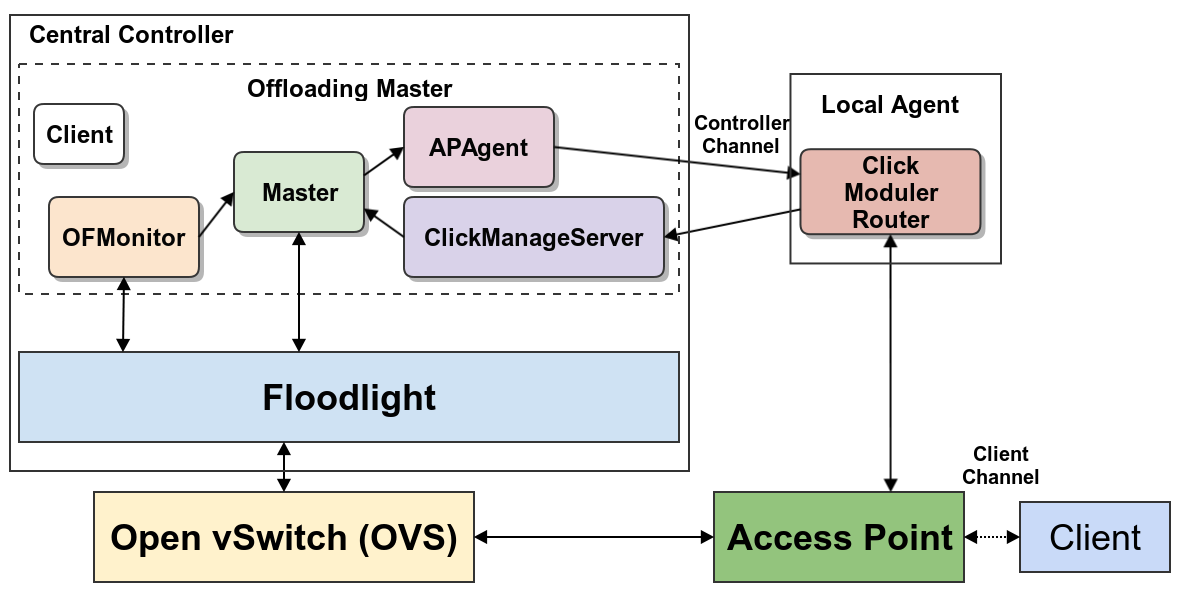
\includegraphics[width=0.85\textwidth]{images/structure.png}
  \caption{Platform Implementation Structure}
  \label{fig:structure}
\end{figure}

\subsubsection{Central Controller}

The central controller manages the whole network, and makes offloading decisions for mobile clients. We implement our central controller with the Floodlight OpenFlow controller, and add the offloading master as an independent application on top of the Floodlight in Java. The offloading master is responsible for traffic offloading management, and the Floodlight controller provides OpenFlow interfaces for updating traffic views on underlying devices.

The current offloading master consists of several different modules, and we show the major ones in Figure \ref{fig:structure}. The Master module is the logical "brain" of the offloading controller. It is responsible to track all the clients and agents appearing in the network, and make decisions related to traffic offloading. The OFMonitor module runs as a separated thread and monitors corresponding OpenFlow switches. If it detects large traffic loads or specific traffic patterns on some switches, it will inform the Master. Both of the Master and the OFMonitor components use Floodlight APIs and OpenFlow protocol to communicate with underlying switches. 
In our current implementation, we choose Linux Laptops running Open vSwitches (sometimes abbreviated as OVS, an open source implementation of virtual switches which support the OpenFlow protocol\footnote[11]{Open vSwitch, \url{http://openvswitch.org/}}) to act as OpenFlow-enabled switches. 

APAgent is an abstract module to represent local agents and store agent information. Some member variables in the APAgent class for WiFi networks are shown in the Listing \ref{lst:APAgent}. The class contains necessary information about a WiFi access point like SSID, BSSID and traffic loads, and is able to extend for different network types. The APAgent also records all the connecting mobile clients and provides necessary functions for the master to interact with access points (e.g. send messages to agents, remove clients, and change channels). The central controller initializes an APAgent instance for each local agent when the system starts up.

Similar to the APAgent class, we use a Client class to represent mobile users. When a mobile user connects to the network, the offloading master initializes a Client instance, and records its information (downloading rate, connect time, and the APAgent which it is connecting to) in the instance. Each mobile user has and only has one corresponding Client instance in the offloading master at one time.

\lstset{language=Java, captionpos=b, caption={WiFi APAgent Class Example -- it includes some basic information and functions for WiFi APs, like SSID and BSSID. The "auth" represents the authentication method of this AP, ofSwitch is the OpenFlow switch which this AP is connecting to, and ofPort is the corresponding connecting port on the OpenFlow switch. All the connecting users on this AP is recorded in clientMap.}, belowcaptionskip=4pt, label=lst:APAgent}
\begin{lstlisting}

public class APAgent implements Comparable<Object> {
    private InetAddress ipAddress;
    private String ssid;
    private String bssid;
    private String auth;
    
    private IOFSwitch ofSwitch;
    private short ofPort;

    private float upRate;
    private float downRate;
    private Map<String, Client> clientMap 
        = new ConcurrentHashMap<String, Client>();
    ......
}
\end{lstlisting}

The ClickManageServer runs as a specific thread listening on a particular port for messages from agents. It collects messages from agents and invokes functions in the Master for different messages. For example, if it receives messages about AP downstream rates, it will inform the master to update corresponding records and data.

\subsubsection{Local Agents}

Local agents run on physical access points, and are implemented with Click modular router \cite{click}. Click is a software architecture for building flexible and modular routers to forward packets. Different packet processing modules (called as elements in Click) can be assembled together for complicated forwarding policies. Individual elements in Click are designed for various functions like packet classification, routing, and monitoring. How packets are processed by a Click router is defined in a configuration file with particular syntax. It indicates which elements are used in the router, and in what sequence they operate on packets. When a Click router starts, it first parses necessary information from a given configuration file, and then process packets according to the configuration.

Since the Click router is quite flexible and well suited for measurement with powerful modular packet processing capabilities, we choose to build our local agent based on it. In general, the agent runs on top of a AP interface in monitoring mode, which allows it to "see" all packets appearing at this interface, and handles those packets with the Click router. Figure \ref{fig:agent} shows the basic structure of a local agent. In our current implementation, we use Linux Laptops with hostapd to act as WiFi access points, and build the Click router on them. Hostapd is a user space daemon for wireless access point servers. It is used to turn a wireless adaptor into a WiFi AP which serves mobile clients with IEEE 802.11 standards.

\begin{figure}[htbp]
  \centering
  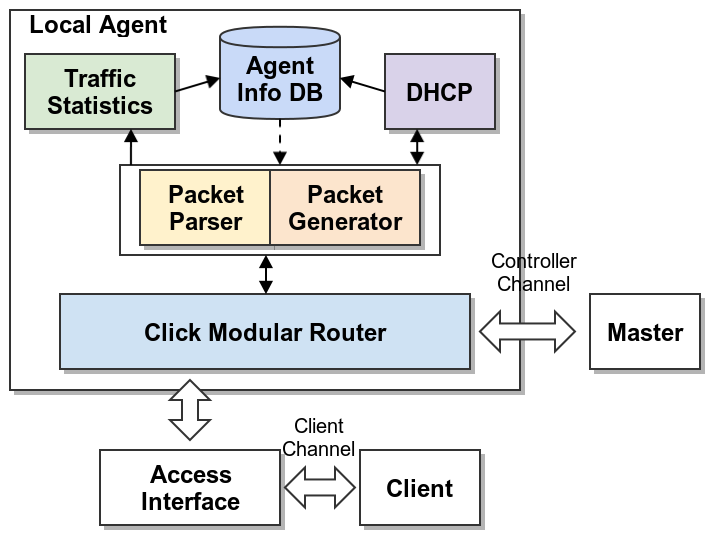
\includegraphics[width=0.8\textwidth]{images/agent.png}
  \caption{Agent Structure -- custom elements (DHCP, statistics and etc.) run on top of the Click modular router.}
  \label{fig:agent}
\end{figure}

As we mentioned in the design section, agents handle client association, and inform the offloading master about client connection/disconnection. To have better control on clients, we develop a custom DHCP server module on Click. Currently agents are responsible to allocate IP addresses for clients. When a client obtains an IP address from an agent, the agent informs the offloading master about this connection. Agents also perform a "keep-alive" testing for each client connecting to it. They periodically send "Ping" packets (ICMP echo request) to the clients. If a client does not reply for two successive "Ping" packets, it is considered as disassociated, and the corresponding agent notifies the master about client disconnection. This mechanism is used for detecting client hand-off, which helps the central controller to have a real-time and accurate view of the whole network.

To record clients and their traffic information, we create a particular data structure to represent mobile users. When a client is connected to an access point, the corresponding Click agent will first initialize a client instance for it, and record necessary information about this client (e.g. IP and MAC address) into the instance. Furthermore, we develop a traffic monitor with Click, which use a shift window to calculate average transmission rate, and record the updated rate for each client in the agent. By tracking all the clients connecting to it, the agent provides great facilities for further procession and client management. 

\subsubsection{Client Extension}

In our platform, clients are also responsible for collecting data, reporting measurements to the controller, and reacting to commands sent from the controller (or agents). To enable these functions, we implement a client extension on user side. This client extension is designed to be general for different mobile operating systems, and we build it on Android devices as an example prototype.

The client extension runs as a background service when started. It listens on a specific port for controlling messages from the master and agents, and reacts to different requests. In its current implementation, the client extension mainly supports the following functions:

\begin{itemize}
  \item WiFi AP Scanning and Reporting: when receiving a scanning request from the controller, the client extension scans nearby WiFi APs, and reports neighboring APs and their signal levels. Scanning results show distances between the client and nearby available APs, which is quite helpful for the offloading decision making. In current Android implementation, this function is implemented with \textbf{\textit{android.net.wifi}} package\footnote[12]{Android-APIs, http://developer.android.com/reference/packages.html}.
  \item Network Switching: the client extension supports to change network connection on mobile devices. If a switching request is received by the client, it will try to disconnect from its current network, and switch to another access point as requested. This is the core function for our offloading, and the central controller can ask clients to connect to specific networks when necessary. This function is also implemented with \textbf{\textit{android.net.wifi}} package.
\end{itemize}
  
The client extension also supports to search specific running applications on mobile devices, and reports them to the controller. The master controller can use this kind of information to decide which clients are more suitable to switch. For example, if services related to YouTube is detected on a mobile device, this mobile client has high possibility to continue generating video streaming traffic. However, it is difficult to cover all kinds of applications on mobile phones, and hard to predict future traffic types only based on these application information. Currently this application matching functionality is still limited to few specific applications, and we are working on improving it with new algorithms.


\subsubsection{Communication Protocol}

To enable efficient communication between the central controller and other components in the system, we develop our own communication protocol. It specifies message meanings for different purposes, and provides a simple mechanism to communicate between the controller and clients with agents as middle proxies. It is currently implemented on UDP. Most of the time, the answer message in our platform can be just in one response packet, and UDP works very well for this kind of simple communication processes. In addition, the system generates newer messages to replace previous ones frequently, so occasional delivering lost is acceptable when low overhead requirements of UDP are considered.

\begin{figure}[htbp]
  \centering
  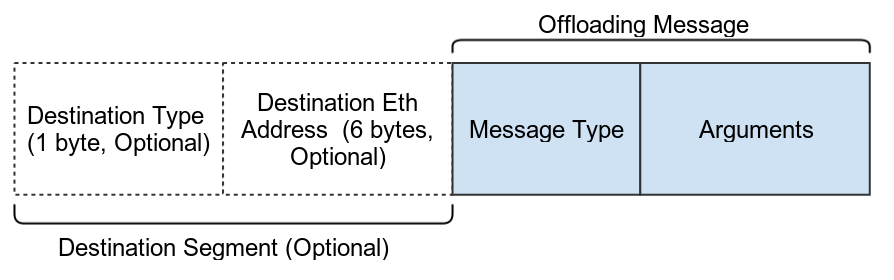
\includegraphics[width=0.9\textwidth]{images/format.png}
  \caption{Message Format}
  \label{fig:format}
\end{figure}


\begin{table}
  \centering
  \begin{tabular}{|p{85pt}|p{80pt}|p{85pt}|p{125pt}|}
    \hline
    \textbf{Message} & \textbf{Arguments} & \textbf{Direction} & \textbf{Description} \\    
    \hline
    
    \verb|REMOVE_CLIENT| & ${\verb|mac_addr|}_{client}$ & Master\ding{213}Agent & Used by the master to inform the agent to remove a client record \\    
    \hline
    
    \verb|CHANGE_CHANNEL| & \verb|new_channel| & Master\ding{213}Agent & Used by the master to inform the agent to change to a different channel \\
    \hline

    \verb|ADD_CLIENT| & ${\verb|mac_addr|}_{client}$, ${\verb|ip_addr|}_{client}$ & Agent\ding{213}Master & Used by the agent to inform the master that a new client has connected \\
    \hline
    
    \verb|AGENT_RATE| & ${\verb|up_rate|}_{agent}$, ${\verb|down_rate|}_{agent}$ & Agent\ding{213}Master & Inform the master the overall traffic rate of this AP during the last time slot \\
    \hline
    
    \verb|CLIENT_RATE| & ${\verb|mac_addr|}_{client}$, ${\verb|up_rate|}_{client}$, ${\verb|down_rate|}_{client}$ & Agent\ding{213}Master & Used by the agent to inform the master the average traffic rate of a specific client during the last time slot \\
    \hline
    
    \verb|DISSC_CLIENT| & ${\verb|mac_addr|}_{client}$ & Agent\ding{213}Master & Used by the agent to inform the master that a specific client has disconnected \\
    \hline
  \end{tabular}
  \caption{Detailed Message Types and Arguments between Agent and Master}
  \label{tab:agent_message}
\end{table}

\begin{table}
  \centering
  \begin{tabular}{|p{65pt}|p{85pt}|p{85pt}|p{140pt}|}
    \hline
    \textbf{Message} & \textbf{Arguments} & \textbf{Direction} & \textbf{Description} \\    
    \hline

    \verb|SWITCH_AP| & \verb|ssid, bssid|, \verb|auth_method|, \verb|auth_password| & Master\ding{213}Client & Used by the master to inform a client to move to a specific AP \\
    \hline
    
    \verb|SCAN_AP| & None & Master\ding{213}Client & Used by the master to inform a client to scan nearby APs \\
    \hline
    
    \verb|QUERY_APP| & None & Master\ding{213}Client & Used by the master to inform a client to report its current running applications \\
    \hline

    \verb|AP_STATS| & (\verb|ssid, bssid|, \verb|signal_level|) & Client\ding{213}Master & Used by the client to report its nearby APs \\
    \hline
    
    \verb|APP_STATS| & \verb|app_name| & Client\ding{213}Master & Used by the client to report its current using applications \\
    \hline
  \end{tabular}
  \caption{Detailed Message Types and Arguments between Client and Master}
  \label{tab:client_message}
\end{table}


A basic message in our protocol consists of one offloading message field and an optional destination segment for agent forwarding. We show this basic message format in Figure \ref{fig:format}. As displayed in the figure, the offloading message part is required, and each message has a message type field and related arguments to indicate its purpose in plain text (ASCII). Table \ref{tab:agent_message} shows messages used between the master and the agent, and messages used between the client and the master are illustrated in Table \ref{tab:client_message}. For example, an agent sends a message with the type of \verb|ADD_CLIENT| to the master when it detects a new mobile user and allocates an IP address to it, and the message also includes MAC address and IP address of that client as arguments. When the controller receives this message, it also records this client and initializes corresponding instant.

The optional destination segment is only used when the master (or a client) sends out messages to another component. Because there is no direct channel between the master and each client, they has to send packets via an agent proxy. This destination field is designed for agents to recognize whether a message is sent to it or needs to be forwarded to another destination. As a result, messages sent directly by agents (e.g. \verb|ADD_CLIENT|, \verb|AGENT_RATE|) do not contain this destination field, and only messages sent by the master or clients include this segment. For example, when the master sends a request message \verb|SCAN_AP| to a client, it adds a destination prefix into the message. This destination segment includes two parts: the Destination Type indicates this packet is sent to a client, and the client MAC address is given in the field of Destination Eth Address. When the agent receives this message, it first interprets the destination from the message. Here the destination is a specific client, so the agent looks up the corresponding IP address for this client based on the given MAC address. Then it removes the destination segment, re-makes a new packet only with the rest part as the offloading message, and sends it to the specific client. Table \ref{tab:dest_seg} describes all the combinations of different destination types and address arguments. 

\begin{table}
  \centering
  \begin{tabular}{|p{55pt}|p{70pt}|p{115pt}|p{135pt}|}
    \hline
    \textbf{Type} & \textbf{Address} & \textbf{Direction} & \textbf{Description} \\    
    \hline

    \verb|TO_AGENT| & None & Master/Client\ding{213}Agent & Used when the master (or a client) sends packets to an agent \\
    \hline
    
    \verb|TO_CLIENT| & ${\verb|mac_addr|}_{client}$ & Master\ding{213}Client & Used when the master sends packets to a client \\
    \hline
    
    \verb|TO_MASTER| & None & Client\ding{213}Master & Used when a client sends packets to its master \\
    \hline
  \end{tabular}
  \caption{Combinations of Different Destination Types and Addresses}
  \label{tab:dest_seg}
\end{table}

\begin{figure}[htbp]
  \centering
  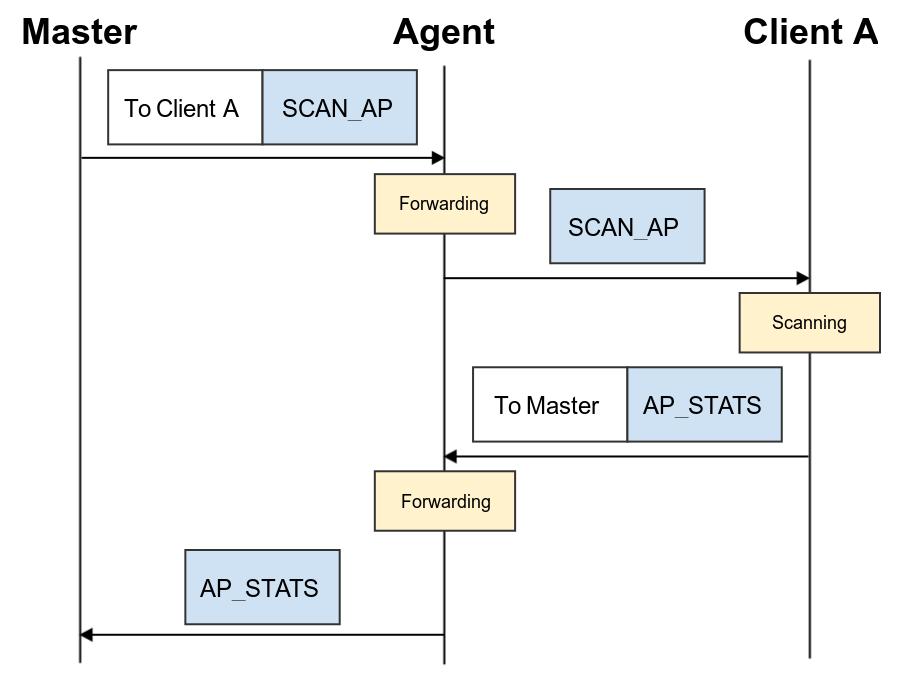
\includegraphics[width=0.8\textwidth]{images/flow.png}
  \caption{Flow Diagram between Master and Client}
  \label{fig:flow}
\end{figure}

Figure \ref{fig:flow} shows a message return round among the master, one middle agent and one client. The master first sends a request to the client via the agent, and asks it to scan nearby access points. As shown in the figure, the agent removes the destination segment, and sends the rest part of the message to client $A$. Client $A$ responses the request with scanning results, and transmits the results to the agent with a destination head pointing to the master. Finally the agent forwards the result contexts to the Master. 


\subsubsection{Realizing Offloading}

In this part, we illustrate the major function of our platform -- traffic offloading, and explain its implementation in details.


\vspace{1mm}

\textbf{Traffic Monitoring}

\vspace{1mm}


There are two ways to start traffic offloading in our system: clients can request the central controller to perform offloading actively for them, or the offloading process is triggered by the traffic monitor in the central controller. If clients try to request offloading by themselves, the central controller will directly start to evaluate offloading destinations for them. However, a more general case is that the traffic monitor initializes the whole offloading process.

The traffic monitor is implemented as the OFMonitor module in our offloading master. It runs as a separated daemon and monitors traffic loads on each access switches with the OpenFlow protocol. In our current implementation, it collects port statistics information on received and transmitted bytes from OpenFlow switches periodically with a fixed interval (typically 2 seconds), and estimated the average transmission rate for each period. If the average rate for a specific AP is higher than a given threshold (e.g. 50\% bandwidth or 70\% bandwidth) consecutively for several times (e.g. $2seconds \times 10times$. We set this parameter based on our experience: if a device generates a large traffic load consecutively for more than 20 seconds, we think it is probably a very active user and may demand more bandwidth resources), the OFMonitor will trigger offloading process for that AP, and start to select clients for potential switching as we explained in Section 4.4.

To eliminate jitter and measure errors in traffic sampling, we design and implement a pending mechanism for monitoring. we use a counter to record the successive times that the average rate is over the given threshold value. When the average rate first surpasses the threshold and then drops down, the counter will not be reset to zero immediately. If we get a large traffic rate later within our pending time window, the counter will grows again from its pending value, instead of from a reset zero value.

\vspace{1mm}

\textbf{Collecting Signal and Bandwidth Information}

\vspace{1mm}


When offloading is triggered and candidate clients are chosen, the system starts to collect location and bandwidth information for each offloading destination. The central controller asks each client to report its signal scanning results, which show distances between the client and its neighboring APs. Then we collect bandwidth information for those APs which are not far away from the client with our local agents. Each local agent records traffic statistics and reports them to the central controller periodically, and the system stores those statistics messages, and estimates bandwidth utilization for each AP.


\vspace{1mm}

\textbf{Short-Term Mobility Prediction for Offloading}

\vspace{1mm}


Besides signal strength, another important type of location information is client potential movement. For example, when a mobile user is getting away from an AP, we may need to avoid choosing this AP for offloading even though the user is near this AP right now. Only collecting static signal information may be misleading for making offloading decisions.

As we know, there have been lots of work related to predict human mobility under various scenarios, but it is still a challenging job in wireless environments. Since we only need short-term prediction on distances between users and specific APs in next few minutes, it is not necessary to have a complex prediction algorithm. Instead of focusing on this hard problem, currently we design and implement a simple mobility prediction mechanism mainly for verify our offloading algorithm and system feasibility. When collecting signal information, we ask clients to perform signal scanning three times during a short time slot (e.g. 5 seconds), and report all the scanning results to the central controller. The controller makes a short-term mobility prediction based on all the scanning results. 

In Section 4.4 (in polynomial \ref{eq:offloading} on page \pageref{eq:offloading}), we use a weight value ($\mu, 0<\mu\leq 1$) to show the influence brought by user movement. Our implemented mobility prediction algorithm tries to calculate this parameter as follows. It compares three signal scanning results for one specific AP (namely $s_1$ for the first scanning result, $s_2$ for the second one, and $s_3$ for the signal strength of the third time), and ranks them with the following classifying algorithm. Each class has an mobility weight, and the further the client is predicted to leave from the AP, the smaller this weight value is.

\begin{enumerate}
  \item Moving Away
  \begin{itemize}
    \item $s_3 \leq s_2 \leq s_1 \land s_3 < s_1$: this can be considered as an apparent pattern of client getting further away, so we assign the minimum value (e.g. 0.7 in our current implementation) to the mobility weight.
    \item $s_1 < s_2 \land s_1 > s_3 $: this shows that the signal level first increases, but finally drops. We give this case a weight value like 0.8, which is a bit better than the previous case.
  \end{itemize}  
  
  \item Approaching
  \begin{itemize}
    \item $s_1 \leq s_2 \leq s_3 \land s_1 < s_3$: this obviously means the mobile user is getting closer to the AP, and we assign the maximum metric value 1 to this case.
    \item $s_1 > s_2 \land s_1 < s_3 $: signal level first drops, but finally increases. We think this is better than moving away, so we assign a value like 0.9 to it. 
  \end{itemize}
  \item Other Conditions: If the result of signal level comparison does not fall into any above categories, we assign a medium value (like 0.85) to it. This category means that there is no clear movement direction detected by the controller, and the user is more likely to still stay around this AP. For example, $s_1 = s_3$ can be classified into this case, and we think it shall get a better weight than the case of moving away. 
\end{enumerate}

Then we use the mobility weight value with other obtained information, like signal strength and bandwidth factors, to calculate the offloading metric of each AP, and make final offloading decisions based on the comprehensive metric values.


\subsection{Evaluation}

In this section, we present an evaluation of our platform. The objective is to understand the practicality of our system, as well as to see different overhead incurred by the system. Our evaluation consists of two major sets of experiments. First, we verify the feasibility of our platform, and demonstrate its benefits in some real-world scenarios by presenting both static and mobility offloading tests. Second, we measure the system performance and overhead, as well as client overhead for offloading. The testing results may be used for determining platform parameters in the future.

\subsubsection{Testbed Description}

\begin{figure}[htbp]
  \centering
  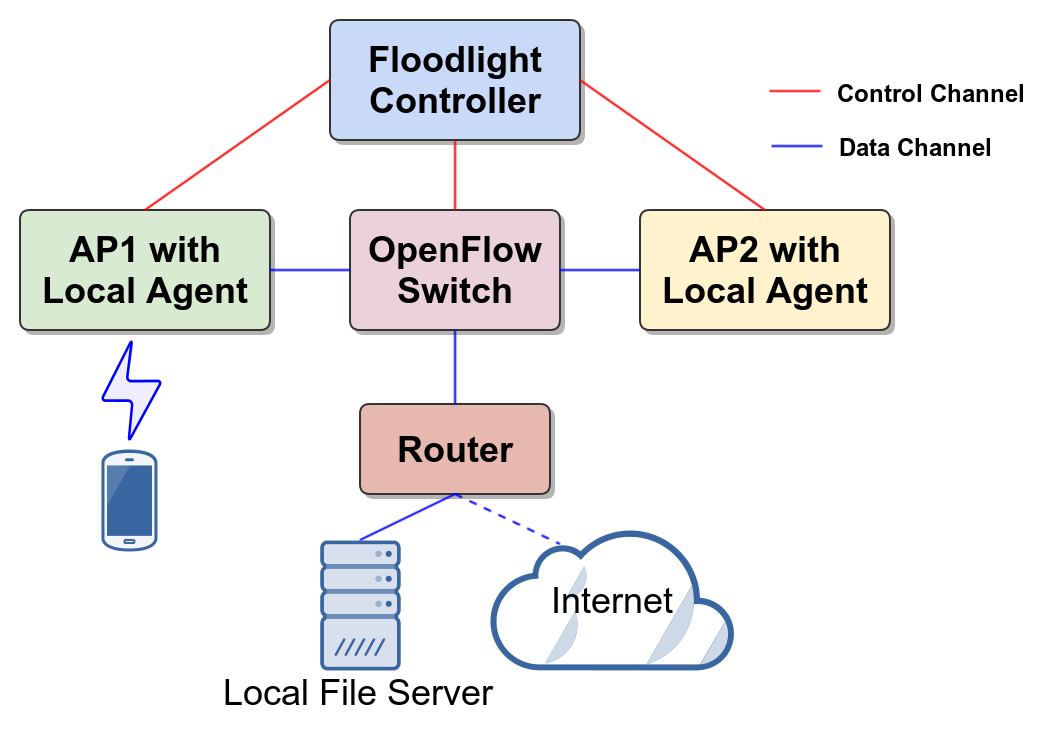
\includegraphics[width=0.7\textwidth]{images/system.png}
  \caption{Basic Structure of Our Implemented Testbed}
  \label{fig:system}
\end{figure}

To evaluate our platform, we set up a small-scale system consisted of two WiFi APs and one central controller, and use it as our main testbed. The basic structure of our testbed is shown in Figure \ref{fig:system}. Since we do not have any manageable 4G base station, we only use WiFi APs in our tests to simulate mobile offloading between different networks. Logically the WiFi APs are just wireless resources to provide different network accesses. Figure \ref{fig:testbed} shows our real implemented testbed in the lab. The Floodlight controller and Open vSwitch(v2.3.0) run on desktop machines (Intel Core Duo E8500 CPU, 6GB RAM, Ubuntu 14.04 LTS with kernel version 3.13.32) as displayed in the picture. Two DELL laptops with hostapd (v2.3) and USB WiFI adapters work as our 802.11n WiFi APs, and run the local agents based on Click v2.0.1. We also use one laptop acting as a router to provide access to the Internet and a local Apache file server for file downloading tests.


\begin{figure}[htbp]
  \centering
  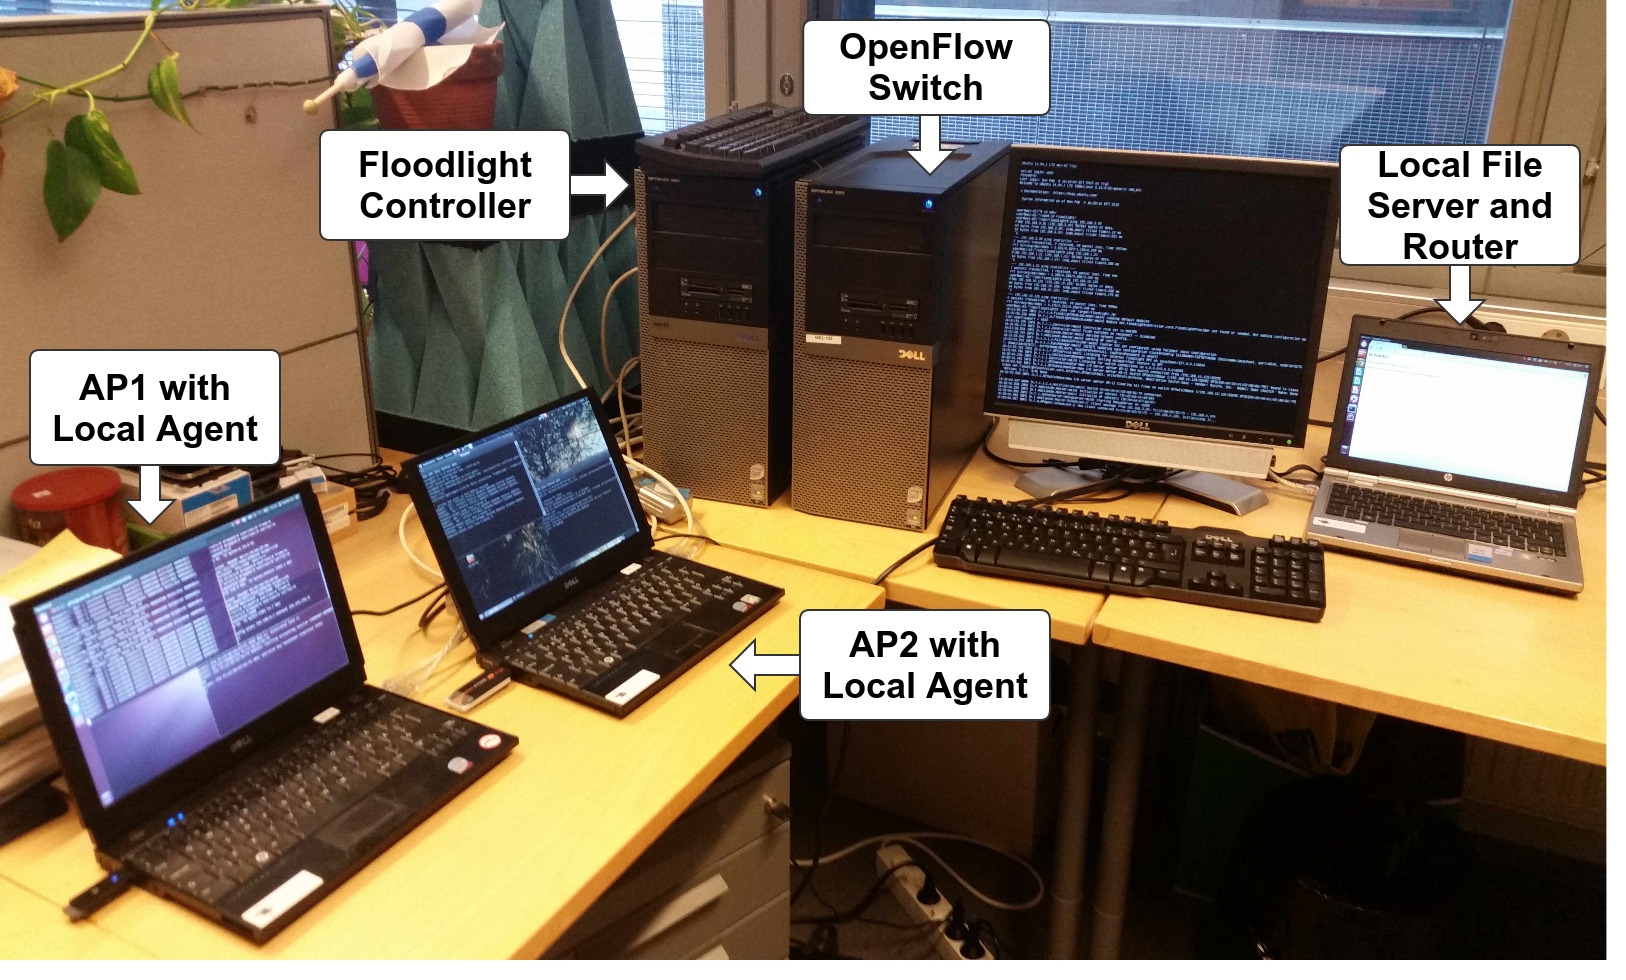
\includegraphics[width=0.75\textwidth]{images/testbed.jpg}
  \caption{Our Implemented Testbed at University of Helsinki}
  \label{fig:testbed}
\end{figure}

\subsubsection{Static Offloading Evaluation}


Our platform offers a mechanism to offload mobile data from one network to another (or one access point to another). As mentioned in Chapter 4, the system shall make offloading decisions with the aim of increasing client throughput and balancing system traffic loads, and avoiding naive traffic offloading. It is important that our system can use different kinds of information, and choose beneficial access points for clients to switch if offloading is necessary and possible. In the following experiments, we validate whether this system satisfy our requirements.


\vspace{1mm}

\textbf{Traffic Detection and Offloading Triggering}

\vspace{1mm}


First of all, we focus on our traffic monitor in the controller, and verify its functionality as well as explore its performances with different monitoring intervals. Since traffic detection is one of the most crucial parts which triggers all of the rest offloading processes, we hope to show its feasibility and try to determine a reasonable monitoring interval parameter for future tests.

We conduct this experiment on our testbed shown in Figure \ref{fig:testbed}: one OpenFlow switch (Open vSwitch) and two APs are connected to the Floodlight controller, and there is one galaxy tab associated to one of the APs. The master maintains states to APs and the OpenFlow switch, as well as the client. In the test, we add a traffic monitoring service in our Android application, and initialize file downloading from the Android application. The traffic monitoring service is based on Android traffic statistics APIs, and periodically calculates mobile data transmission rate with a very short interval (0.2s). When it first detects an average downlink speed higher than 2 Mbps, the Android application reports that rate to our central controller. The central controller also performs its own traffic monitoring on the OF switch. We compare those two detection times and calculate the detection latency on the master controller. 

\begin{table}[htbp]
\centering
\begin{tabular}{|c|l|l|l|}
  \hline
  Controller Monitoring Interval (s) & \multicolumn{3}{c|}{Detection Latency (s)} \\
  \cline{2-4}
  & Min & Max & Average \\
  \hline
  2 & 0.597 & 2.099 & 1.175 \\
  \hline
  1 & 0.243 & 0.977 & 0.614 \\
  \hline
  0.5 & 0.115 & 0.465 & 0.264 \\
  \hline
\end{tabular}
\caption{Detection Latency with Different Monitoring Intervals -- there is always a small detection delay in the central controller.}
\label{tab:interval}
\end{table}

The experimental results are described in Table \ref{tab:interval}. As we can see, our system can detect specific traffic patterns with a short delay time, and trigger the rest offloading processes successfully. The current implementation introduces a small but visible detection latency on the controller, which approximately equals to the half of the monitoring interval value. For example, when our monitoring interval is set to be 2 seconds, the average detection delay is about 1 second. If the monitoring interval is 0.5 second, we get an average latency of 0.26. The smaller the monitoring interval, the smaller the detection latency. However, when we choose a very small interval, the system will be more sensitive to traffic rate variation. Our traffic monitor will trigger offloading only if the average rate for a specific AP is higher than a given threshold consecutively for several times. In some cases, traffic fluctuates in burst when rate shaping is applied, and offloading trigger may be delayed when we use a very small interval value. So we prefer to select a medium interval, like two seconds, to obtain better monitoring tolerant on rate variation and acceptable detection delays.


\vspace{1mm}

\textbf{Context-based Offloading for Static Clients}

\vspace{1mm}

As one of the most important requirements, our system shall be able to use various context information on wireless environments, and make beneficial offloading decisions. To validate this, we conduct a comparison experiment on our platform.  First, we run our test in a "naive" offloading system, which performs offloading without considering bandwidth and signal strength information. Then we repeat the same evaluation on our offloading system, and compare test results with each other. To simplify this test, user movement is not considered during the whole test, and the clients are kept static and almost moveless.

We carry out the experiment with the same testbed shown in Figure \ref{fig:testbed}, and enable rate shaping on both of the APs. AP1 is limited to provide only 8 Mbps maximum bandwidth to each client, and AP2 is configured with different bandwidth values from 4 Mbps to 24 Mbps during the experiment. First, we connect our testing tablet to AP1, and perform file downloading from the local file server. In the first round, we use a "naive" offloading decision making algorithm: when offloading is triggered, the client is forced to switch to a different AP without considering context information like bandwidth values. We also change the offloading triggering mechanism in our system for the test. No matter how many clients there are, the system will request the client to switch if it continues to generate downstream traffic exceeding 5.6 Mbps ($70\% \times 1$Mbps, 2-second interval, 7-time consecutive detection). During the switching process, file downloading pauses shortly, and recovers soon after the client connects to another AP.

We record client downloading time for different bandwidth configuration on AP2, and compare those values with a baseline time without offloading. The test results are described in Table \ref{tab:offloading}. If we force the client to naively switch to another AP working with a lower bandwidth value, like here 4 Mbps, the downloading performance will drop with no doubt. It takes more time to finish file transmission, and probably costs more energy. In addition, even if the client switches to an AP with equal bandwidth (8 Mbps), the downloading performance still drops due to offloading overhead.

\begin{table}[htbp]
\centering
\begin{tabular}{|p{130pt}|p{70pt}|p{70pt}|p{70pt}|}
  \hline
  & \multicolumn{3}{c|}{Avg Time for Downloading(s)} \\
  \cline{2-4}
  & 33 MB File & 65 MB File & 141 MB File \\
  \hline
  Stay on AP1 (8Mbps) & 34.333 & 65.526 & 141.486 \\
  \hline
  Switch to AP2 (4Mbps) & 49.585 & 115.436 & 267.825 \\
  \hline
  Switch to AP2 (8Mbps) & 36.284 & 68.393 & 145.432 \\
  \hline
  Switch to AP2 (16Mbps) & 34.377 & 49.732 & 88.456 \\
  \hline
  Switch to AP2 (24Mbps) & 32.590 & 43.834 & 70.610 \\
  \hline
\end{tabular}
\caption{Download Performance with Naive Offloading -- we use the results when the client stays on AP1 as a baseline performance, and it is obvious to see that the average downloading time increases when client is switched to an AP with a lower bandwidth value.}
\label{tab:offloading}
\end{table}

\begin{table}
  \centering
  \begin{tabular}{|c|c|}
    \hline
    AP2 Bandwidth Config & Offloading Decision \\
    \hline
    4Mbps & not switch \\
    \hline 
    8Mbps & not switch \\
    \hline 
    16Mbps & switch to AP2 \\
    \hline 
    24Mbps & switch to AP2 \\    
    \hline
  \end{tabular}
  \caption{Offloading Decisions for different AP configurations -- this time, we apply our offloading decision making algorithm. The controller avoid offloading data to non-beneficial APs.}
  \label{tab:decisions}
\end{table}

Next, we repeat the same test with our offloading decision making module, and record final offloading decisions in this round. The results of our experiment is described in Table \ref{tab:decisions}. As it shows, our system can use bandwidth information from managed APs, and avoid offloading data to non-beneficial destinations. When AP2 works with a lower bandwidth like 4 Mbps, no offloading will be performed. When two APs provide the same bandwidth (8 Mbps), the final decision of our algorithm is still not switching, because we take the offloading overhead into account. In the test, we set the offloading overhead weight $c_2$ (in polynomial \ref{eq:offloading} on page \pageref{eq:offloading}) to be 0.2. If AP2's bandwidth is 16 Mbps, higher than AP1's current value, the client will be asked to switch from AP1 to AP2.

One thing to note here is the offloading overhead. Even when the client connect to a "better" AP with higher bandwidth, the downloading time and energy consumption may still increase due to the switching overhead. WiFi scanning and reconnection both take extra time and energy, and that is why we introduce the offloading overhead metric in our decision making process. For example, even the client switches to the AP with a 16 Mbps bandwidth, the total duration for fetching a 33MB file increases from 34.33s to 34.37s. Though we have considered the switching overhead, it is still very difficult to predict future traffic types and amount for mobile clients. However, if clients continue to use APs with better bandwidth, it will definitely enjoy benefits of offloading.

In addition to bandwidth, our system can utilize location information based on signal strength. Constrained by our office testbed, we use a data-based simulation to verify our system's reactions to signal information. We repeat our tests with different distances from the client tablet to the APs, and observe what the signal strength values are, and how the controller responses to different signal levels. As what we expect, the controller can obtain correct signal strength information from the client, and calculate offloading metric values based on this information. The system can avoid offloading data to a far-away AP.


\vspace{1mm}

\textbf{Combining Bandwidth and Signal Information in Offloading Decision}

\vspace{1mm}

In the previous experiments, we have evaluated system reactions on the bandwidth and signal information respectively. Next, we try to consider them together, and take a look at how our controller handles multi-type context information. As we explained in Chapter 4, both of the bandwidth values and signal levels affect real transmission throughput, and we formulate a throughput metric based on these two factors (detailed explanation in polynomial \ref{eq:offloading} on page \pageref{eq:offloading}):

$$(1 - e^{-k_0(S - k_1)}) \cdot  \frac{estimatedB_a}{\operatorname*{arg\,max}_a estimatedB_a} \cdot \frac{restB_a}{totalB_a}$$

where $S$ is the received signal level collected from the client side, and $B_a$ is the bandwidth parameter of AP $a$. Based on our previous measurement, we set $k_0 = \frac{1}{3}$, and $k_1 = -73$. To evaluate this throughput metric in the controller, we perform a data-based verification in our office testbed. In this test, we only use one client. First, we set up one AP with different bandwidth settings, and repeat downloading the same file from various locations. We record the download speed for each combination of bandwidth and signal parameters, and then verify throughput metric used in our offloading system based on our measurement data.

\begin{table}[htbp]
\centering
\begin{tabular}{|p{35pt}|p{84pt}|p{50pt}|p{35pt}|p{84pt}|p{50pt}|}
  \hline
  \multicolumn{3}{|c|}{Bandwidth = 8Mbps} & \multicolumn{3}{c|}{Bandwidth = 16Mbps} \\
  \hline
  Signal (dBm) & Avg Throughput (Mbps) & Offloading Metric & Signal (dBm) & Avg Throughput (Mbps) & Offloading Metric \\
  \hline
  -31 & 7.84 & 0.500 & -34 & 15.12 & \textbf{1.000} \\
  \hline
  -65 & 7.52 & 0.465 & -66 & 15.04 & \textbf{0.903} \\
  \hline
\end{tabular}
\caption{Downloading Test with Different Bandwidth and Distance Settings -- the bandwidth value is configured for each client connection. When signals are at similar levels, the metric value is mainly determined by bandwidth parameters.}
\label{tab:combination-test-1}
\end{table}

\begin{table}[htbp]
\centering
\begin{tabular}{|p{35pt}|p{84pt}|p{50pt}|p{35pt}|p{84pt}|p{50pt}|}
  \hline
  \multicolumn{3}{|c|}{Bandwidth = 8Mbps} & \multicolumn{3}{c|}{Bandwidth = 16Mbps} \\
  \hline
  Signal (dBm) & Avg Throughput (Mbps) & Offloading Metric & Signal (dBm) & Avg Throughput (Mbps) & Offloading Metric \\
  \hline
  -31 & 7.84 & 0.500 & -75 & 3.68 & \textbf{-0.947} \\
  \hline
  -65 & 7.52 & 0.465 & -78 & 3.04 & \textbf{-4.294} \\
  \hline
\end{tabular}
\caption{Downloading Test with Different Bandwidth and Distance Settings: when signal strength drops to -75 dBm, the real throughput drops from 16 Mbps to 3.68 Mbps, which is even worse than downloading the same file via an AP only with 8 Mbps bandwidth, but better signal strength.}
\label{tab:combination-test-2}
\end{table}

The baseline results of the downloading test and our calculated throughput metric values are described in Table \ref{tab:combination-test-1} and Table \ref{tab:combination-test-2}. The larger the metric value is in the table, the better this AP is considered for offloading. As shown in the tables, our current throughput evaluation model can give a notably accurate metric for future offloading. If both of the APs have good signal levels above -70 dBm, the one with better bandwidth setting probably provides better transmission throughput to clients, just like what is described in Figure \ref{tab:combination-test-1}. However, when the signal strength drops below a specific threshold, the throughput decreases steeply. In our test, the average throughput drops from configured 16 Mbps to 3.04 Mbps if the signal strength is below -75 dBm. It is even worse than the speed to transmit data from the AP with only 8 Mbps bandwidth, but a -65 dBm signal level. Our mathematical model identically show this trend: even when the configured bandwidth is better, we may still get a worse throughput metric value with a poor signal level. As displayed in the table, it drops to a negative value when the signal level is -75 dBm, which is much smaller than the throughput metric 0.465 of the AP with only 8 Mbps bandwidth but a -65 dBm signal level. 

The test result illustrates that our mathematical model accurately fits the real throughput variation due to signal and bandwidth changing, and the system is able to make good offloading decisions based on the mathematical model.


\vspace{1mm}

\textbf{Summary}

\vspace{1mm}


All the experiments illustrated in this section demonstrate that our system can successfully trigger offloading with the current monitoring mechanism, and make beneficial offloading decisions based on real bandwidth configuration, traffic situations and signal levels for static clients.


\subsubsection{Mobility Prediction Evaluation}


In the previous section, we verify the offloading functionality in a nearly moveless environment. The test results show that our system can perform well in static scenarios. For example, users stay at office when they use mobile devices. However, a more common and realistic situation is that users are moving when the system makes offloading decisions. In our platform, we design and implement a simple mobility prediction mechanism. The following experiment is aimed at validating this prediction module, and understand its influence on offloading decision making.

We use a similar offloading setup as in the previous experiment, but locate the two APs at different sides of our office with a 4-meter distance. This allows us to make different movement trajectories between these two APs in our office. The APs are configured with the same parameters including the bandwidth and WiFi channels. We use the Galaxy tab and our Android testing application to download a local file from one AP, and try to trigger system traffic offloading. Then we hold the tab and make different movement trajectories in our office, and observe how our system reacts to the movement. In the current implementation, the central controller tries to collect clients' mobility information only before it makes offloading decisions, so our movement is mainly performed during the time that the central controller collects mobility data.

\begin{figure}[htbp]
  \centering
  \subfloat[walk straight from AP1 to AP2]{
    \label{fig:mobility1}
    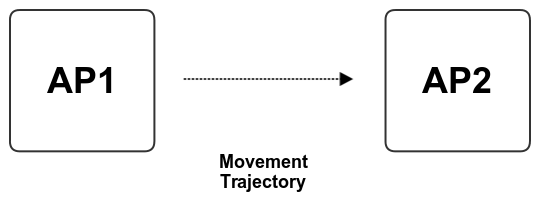
\includegraphics[width=0.4\textwidth]{images/mobility1.png}
  }
  \hspace{10 pt}%
  \subfloat[make a u-turn and back to AP1]{
    \label{fig:mobility2}
    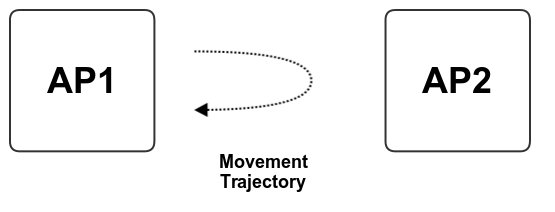
\includegraphics[width=0.4\textwidth]{images/mobility2.png}
  }
  \caption{Movement Trajectories}
  \label{fig:mobility}
\end{figure}

The testing topology and our movement trajectories are shown in Figure \ref{fig:mobility}. Before moving, we first connect our testing tab to AP1, and stand near AP1. In case (a), we walk straight (or straight-like) from AP1 to AP2. In case (b), we first move from AP1 to AP2, and then make a u-turn back to AP1. These two movement trajectories show two of the most common cases in the real world. In both of the cases, we repeat our test at an average walking speed of about 1m/s. 

Table \ref{tab:mobility} describes our test result measured in average accuracy. As we can see, there are two kinds of accuracy values in the table. In our design model, we use $\mu \cdot (1 - e^{-k_0(S - k_1)})$ to evaluate influences of signal levels and user mobility (detailed explanation in polynomial \ref{eq:offloading} on page \pageref{eq:offloading}), and here the accuracy of mobility prediction illustrates whether our system can give an accurate prediction of $\mu$ in the test. We only think our predicted $\mu$ is accurate when it exactly matches our movement trajectory. For example, when we move from AP1 to AP2 in case (a), the prediction result is accurate only if it reports that we are getting closer to the AP2, and further away from AP1 (e.g. ${\mu}_{AP1} = 0.7,\; {\mu}_{AP2} = 1$). Other types of forecast results we mentioned in Section 5.5 (e.g. unclear movement direction) are considered inaccurate. 

The overall accuracy considers all the factors in $\mu \cdot (1 - e^{-k_0(S - k_1)})$, and shows how our system performs on a comprehensive prediction with signal levels and mobility. As we can see from our model, the potential mobility and signal levels are used together to evaluate user throughput. Take the same example, if we move from AP1 to AP2 in our test, the overall metric of AP2 shall be larger than that of AP1 in an accurate prediction. 

\begin{table}
  \centering
  \begin{tabular}{|p{50pt}|p{120pt}|p{150pt}|}
    \hline
    & Accuracy of Mobility Prediction & Overall Accuracy with Mobility Prediction and Signal Level \\    
    \hline
    Straight & 60\% & 90\% \\
    \hline
    U-Turn & 65\% & 90\% \\
    \hline
  \end{tabular}
  \caption{Mobility Prediction Evaluation}
  \label{tab:mobility}
\end{table}


In the experiment, our simple mobility prediction module does not provide a very accurate forecast on user movement. Sometimes it may even gives quite misleading prediction on user's moving trajectories due to measurement error. However, when we use it together with signal strength, as our evaluation algorithm requires, the offloading controller can make correct offloading choices in most of the times. As displayed in the table, the overall evaluation accuracy of our system reaches to 90\% when we move during the test. In a word, our system can also perform well and make correct offloading decisions when a short-term mobility prediction is required.

\subsubsection{Controller Overhead}

In this experiment, we compare monitoring performance with different intervals, and observe corresponding CPU and memory overhead on the central controller. By exploring the basic performance of our central controller, we hope to show that the controller can operate with acceptable overhead for a common-size deployment.

\begin{figure}[htbp]
  \centering
  \subfloat[CPU Utilization and Monitoring Interval]{
    \label{fig:interval-cpu}
    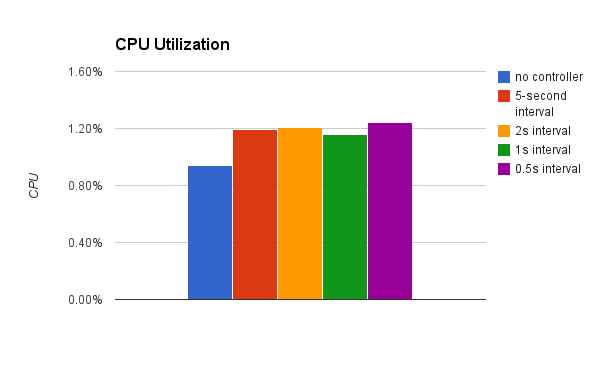
\includegraphics[width=0.75\textwidth]{images/interval-cpu.png}
  }
  \hspace{5pt}%
  \subfloat[Mem Utilization and Monitoring Interval]{
    \label{fig:interval-mem}
    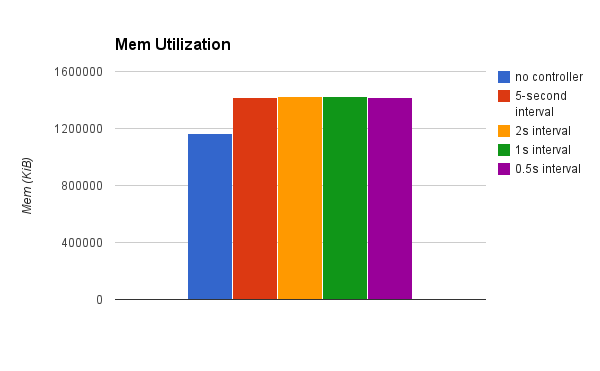
\includegraphics[width=0.75\textwidth]{images/interval-mem.png}
  }
  \caption{System Overhead with Different Monitoring Intervals}
  \label{fig:interval}
\end{figure}

The experimental setup is the same as what we used in the previous tests: one OpenFlow switch (Open vSwitch) and two APs are connected to the Floodlight controller, and one galaxy tab associated to one of the APs. We observe the CPU and memory overhead on the central controller. We also record the CPU and memory utilization when our Floodlight controller does not start up as a baseline benchmark. As shown in Figure \ref{fig:interval}, when the Floodlight starts up on our testing machine (Intel Core Duo E8500 CPU, 6GB RAM, Ubuntu 14.04 LTS with kernel version 3.13.32), it does bring some overhead, but reasonable and stable: 250 MB memory, and nearly 0.3\% more CPU utilization. When we shorten the monitoring interval, the system overhead does not vary much. These results show that the overhead introduced by our controller is reasonable even when we use a small traffic monitoring interval.


\subsubsection{Client-Side Overhead}

To collect information from the client side, we add client extensions on mobile devices in our system, which brings extra overhead and energy consumption. In this section, we explore the overhead associated with running our client extension on different mobile devices, and check whether it is reasonable and acceptable.

First, we use the original application manager in Android and several benchmark tools available in Google Play to observe the CPU and memory overhead. The results show that our extension stably costs around 30 MB memory on an Android device (Android 4.1+), and nearly no extra CPU overhead when it just runs in the background to listen on messages from a specific port. The CPU utilization increases only when the client extension performs specific measurement and controlling tasks which are requested by the controller (e.g. WiFi scanning and network switching). 

\begin{figure}[htbp]
  \centering
  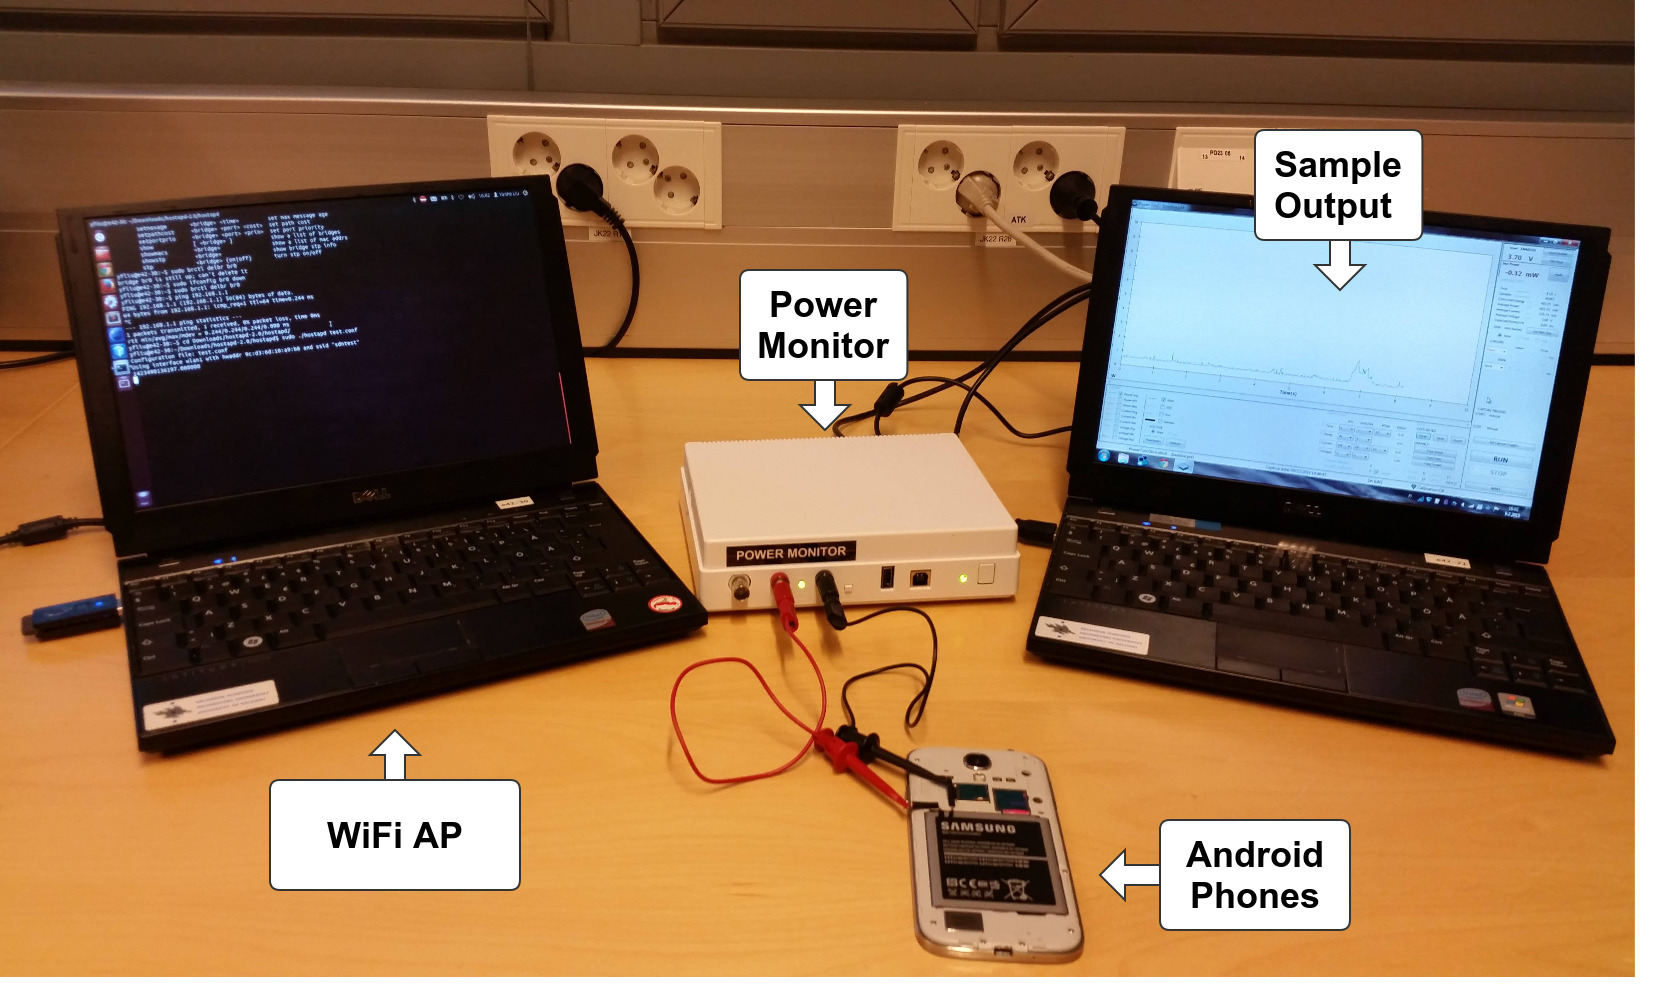
\includegraphics[width=0.8\textwidth]{images/client-overhead.jpg}
  \caption{Testbed for Recording Client Overhead on Scanning and Switching -- we send specific management commands from the WiFi AP, and estimate extra energy consumption on the client device. This test setup is exactly the same as the one shown in Figure \ref{fig:signal-level-topo}.}
  \label{fig:client-overhead}
\end{figure}

To derive extra client overhead caused by responding specific commands, we conduct two tests for WiFi scanning and network switching respectively. The test setup is exactly the same as those used in Chapter 4. In the experiment, we send management commands from the WiFi AP to trigger WiFi scanning or network switching, and then start recording energy consumption on mobile devices by using the power monitor shown in Figure \ref{fig:client-overhead}. Here we mainly focus on energy consumption, because it is a major concern on every mobile device and directly shows real-world overhead. We also observe average baseline energy consumption on each different devices, and estimate extra overhead consumption by subtracting the baseline value.


\begin{table}[htbp]
\centering
\begin{tabular}{|l|p{50pt}|p{100pt}|p{50pt}|p{100pt}|}
  \hline
  & \multicolumn{2}{c|}{WiFi Scanning} & \multicolumn{2}{c|}{Network Switching} \\
  \cline{2-5}
  & Time (s) & Energy Consumption (uAh, 3.7V) & Time (s) & Energy Consumption (uAh, 3.7V)\\
  \hline
  Galaxy S1 & 4.58 & 84.63 & 2.004 & 94.88 \\
  \hline
  Galaxy S2 & 14.66 & 356.21 & 1.35 & 180.19 \\
  \hline
  Galaxy S3 & 13.56 & 235.97 & 1.01 & 62.54 \\
  \hline
  Galaxy S4 & 13.23 & 299.67 & 1.22 & 83.55 \\
  \hline
  Galaxy S5 & 13.04 & 454.91 & 1.04 & 77.79 \\
  \hline
\end{tabular}
\caption{Client Overhead of WiFi Scanning and Switching}
\label{tab:overhead}
\end{table}


The testing results are shown in Table \ref{tab:overhead}. Switching to a different WiFi network takes about 1.2 seconds, and around 80 uAh on most of the devices (Association may take more time if the user is in a very radio-noisy environment). Typically a battery on a current Android mobile phone is around 2500 mAh (3.7V), and the average extra energy consumption of switching is equivalent to the cost when mobile screen is turn on for approximately 3 seconds. Since connecting to WiFi goes through several steps like wireless association and IP address acquiring, this average time and energy value are definitely acceptable. 

Much to our surprise, the WiFi scanning -- another very important process in offloading, takes around 13 seconds on several new Galaxy devices. In the previous offloading tests, we use tablets (Galaxy tab 2) and did not suffer from this problem. They finish scanning in about 4 seconds, just like Galaxy S1. Currently we still haven't figured out the reason to this problem, but it shows that our simple mobility prediction algorithm may be not feasible. It takes too much time to finish the 3-time signal scanning, and clients may have already missed appropriate opportunities for offloading. Though it may be possible to fix this problem by hacking Android underlying code or chip drivers, a more practical way is to change our current mechanism on mobility prediction.



\subsection{Discussion}

The evaluation demonstrates the feasibility and practicality of our prototype implementation in WiFi networks. Our system works well for static clients and makes accurate decisions based on some context information. However, the test results also show some potential problems, and we discuss them in this section.

\vspace{1mm}

\textbf{Offloading Mobility Prediction}

\vspace{1mm}

The experiment data on client overhead show that our current mobility prediction algorithm and implementation may not work for some new devices. For example, it takes about 13 seconds to finish 3-time WiFi scanning on Samsung Galaxy S5, which is too long and makes offloading impractical. In addition, it treats all different users as the same type, and request all of them to perform multi-time scanning. This may be also unnecessary and inefficient. In one word, we may need to design a new mechanism to quickly give short-term movement prediction on all kinds of devices when it is necessary.

\vspace{1mm}

\textbf{Cellular Testing}

\vspace{1mm}

In our current implementation, cellular access points are simplified and abstracted as the same wireless resources as WiFi access points, and we only use WiFi networks to show our system's feasibility. Although we try to design a general system for different networks, further tests on an extended platform both with WiFi and cellular access points are required. Cellular and WiFi are still different techniques, and there may be some limitations and requirements only appearing in cellular networks. 



\newpage

\section{Conclusion and Future Work}

In this paper, we consider the traffic offloading problem and propose an SDN-based system which performs offloading by utilizing different kinds of wireless context information. The system design is motivated by a real-world measurement study on wireless network accesses. To make beneficial offloading decisions not only for the system, but also for clients, our system collects information from two sides and evaluates them in a comprehensive way. The feasibility and practicality of our design system are verified through a prototype implementation, and we demonstrate its performance and overhead with real-world test cases. The evaluation results show that our proposal system may achieve optimal offloading by considering various factors, and avoid "naive" offloading.

In addition to context-based offloading decision making, we explore the idea of managing networks in a software-based approach, and develop our system with SDN techniques. By expressing different functions as software applications, we demonstrate that it is easy to introduce new ideas and turn them into reality in an SDN system like our platform.

As the first step to the software-based traffic offloading, there are still some problems, as well as possibilities in our current system. We leave them as future work, and hope to solve them later:

\begin{itemize}
  \item Mobility Prediction: our current offloading mobility prediction brings so long latencies on some new Android devices that additional support is required. Furthermore, we treat all devices as the same type and perform identical 3-time scanning, which may be inefficient and inaccurate on some devices. For example, the 3-time scanning costs extra energy but is probably unnecessary for static clients. Users with vehicular mobility shall avoid WiFi switching because it brings more limited coverage. We shall not only modify current prediction algorithm, but distinguish different types of users in the future work.
  \item Cellular Network Evaluation: In our current implementation, no cellular access point is really deployed and tested. Though we emphasize that our design system is general and shall support different network types, further evaluation and validation are still necessary. Porting our current local agents to cellular base stations may also raise some new requirements.
  \item Bandwidth Prediction: As one of the key features in our platform, the controller is able to make offloading decisions based on AP bandwidth information. However, we only collect real-time bandwidth data before user switches networks, which may be not enough. For example, if a client is first moved to an idle AP in one room, then a crowd of users rush in and connect to this AP, the first client may still suffer from lower bandwidth. To avoid this problem, we may need to perform short-term bandwidth and traffic prediction for each AP. Currently we are work on this issue, and try to explore whether we can make more accurate offloading decisions with a history-based traffic prediction.
  \item Scalability: the current prototype implementation only involves 2 controllable APs and one OpenFlow switch. If the size of a network continues to increase, system overhead and resource costs for the central controller to manage the network can be expensive. The scalability shall be explored in our future work.
  \item Other Applications: there are many possible extensions for our platform, e.g. traffic monitoring and access control. As one of our future tasks, we plan to explore practical mechanisms for dynamically channel adjustment on our platform. 
\end{itemize}


\newpage

\nocite{*}
\bibliographystyle{tktl}
\bibliography{lahteet}

\lastpage

\end{document}


